\documentclass[]{book}
\usepackage{lmodern}
\usepackage{amssymb,amsmath}
\usepackage{ifxetex,ifluatex}
\usepackage{fixltx2e} % provides \textsubscript
\ifnum 0\ifxetex 1\fi\ifluatex 1\fi=0 % if pdftex
  \usepackage[T1]{fontenc}
  \usepackage[utf8]{inputenc}
\else % if luatex or xelatex
  \ifxetex
    \usepackage{mathspec}
  \else
    \usepackage{fontspec}
  \fi
  \defaultfontfeatures{Ligatures=TeX,Scale=MatchLowercase}
\fi
% use upquote if available, for straight quotes in verbatim environments
\IfFileExists{upquote.sty}{\usepackage{upquote}}{}
% use microtype if available
\IfFileExists{microtype.sty}{%
\usepackage{microtype}
\UseMicrotypeSet[protrusion]{basicmath} % disable protrusion for tt fonts
}{}
\usepackage[margin=1in]{geometry}
\usepackage{hyperref}
\hypersetup{unicode=true,
            pdftitle={Piecemeal R},
            pdfauthor={Kota Minegishi},
            pdfborder={0 0 0},
            breaklinks=true}
\urlstyle{same}  % don't use monospace font for urls
\usepackage{natbib}
\bibliographystyle{apalike}
\usepackage{color}
\usepackage{fancyvrb}
\newcommand{\VerbBar}{|}
\newcommand{\VERB}{\Verb[commandchars=\\\{\}]}
\DefineVerbatimEnvironment{Highlighting}{Verbatim}{commandchars=\\\{\}}
% Add ',fontsize=\small' for more characters per line
\usepackage{framed}
\definecolor{shadecolor}{RGB}{248,248,248}
\newenvironment{Shaded}{\begin{snugshade}}{\end{snugshade}}
\newcommand{\KeywordTok}[1]{\textcolor[rgb]{0.13,0.29,0.53}{\textbf{{#1}}}}
\newcommand{\DataTypeTok}[1]{\textcolor[rgb]{0.13,0.29,0.53}{{#1}}}
\newcommand{\DecValTok}[1]{\textcolor[rgb]{0.00,0.00,0.81}{{#1}}}
\newcommand{\BaseNTok}[1]{\textcolor[rgb]{0.00,0.00,0.81}{{#1}}}
\newcommand{\FloatTok}[1]{\textcolor[rgb]{0.00,0.00,0.81}{{#1}}}
\newcommand{\ConstantTok}[1]{\textcolor[rgb]{0.00,0.00,0.00}{{#1}}}
\newcommand{\CharTok}[1]{\textcolor[rgb]{0.31,0.60,0.02}{{#1}}}
\newcommand{\SpecialCharTok}[1]{\textcolor[rgb]{0.00,0.00,0.00}{{#1}}}
\newcommand{\StringTok}[1]{\textcolor[rgb]{0.31,0.60,0.02}{{#1}}}
\newcommand{\VerbatimStringTok}[1]{\textcolor[rgb]{0.31,0.60,0.02}{{#1}}}
\newcommand{\SpecialStringTok}[1]{\textcolor[rgb]{0.31,0.60,0.02}{{#1}}}
\newcommand{\ImportTok}[1]{{#1}}
\newcommand{\CommentTok}[1]{\textcolor[rgb]{0.56,0.35,0.01}{\textit{{#1}}}}
\newcommand{\DocumentationTok}[1]{\textcolor[rgb]{0.56,0.35,0.01}{\textbf{\textit{{#1}}}}}
\newcommand{\AnnotationTok}[1]{\textcolor[rgb]{0.56,0.35,0.01}{\textbf{\textit{{#1}}}}}
\newcommand{\CommentVarTok}[1]{\textcolor[rgb]{0.56,0.35,0.01}{\textbf{\textit{{#1}}}}}
\newcommand{\OtherTok}[1]{\textcolor[rgb]{0.56,0.35,0.01}{{#1}}}
\newcommand{\FunctionTok}[1]{\textcolor[rgb]{0.00,0.00,0.00}{{#1}}}
\newcommand{\VariableTok}[1]{\textcolor[rgb]{0.00,0.00,0.00}{{#1}}}
\newcommand{\ControlFlowTok}[1]{\textcolor[rgb]{0.13,0.29,0.53}{\textbf{{#1}}}}
\newcommand{\OperatorTok}[1]{\textcolor[rgb]{0.81,0.36,0.00}{\textbf{{#1}}}}
\newcommand{\BuiltInTok}[1]{{#1}}
\newcommand{\ExtensionTok}[1]{{#1}}
\newcommand{\PreprocessorTok}[1]{\textcolor[rgb]{0.56,0.35,0.01}{\textit{{#1}}}}
\newcommand{\AttributeTok}[1]{\textcolor[rgb]{0.77,0.63,0.00}{{#1}}}
\newcommand{\RegionMarkerTok}[1]{{#1}}
\newcommand{\InformationTok}[1]{\textcolor[rgb]{0.56,0.35,0.01}{\textbf{\textit{{#1}}}}}
\newcommand{\WarningTok}[1]{\textcolor[rgb]{0.56,0.35,0.01}{\textbf{\textit{{#1}}}}}
\newcommand{\AlertTok}[1]{\textcolor[rgb]{0.94,0.16,0.16}{{#1}}}
\newcommand{\ErrorTok}[1]{\textcolor[rgb]{0.64,0.00,0.00}{\textbf{{#1}}}}
\newcommand{\NormalTok}[1]{{#1}}
\usepackage{longtable,booktabs}
\usepackage{graphicx,grffile}
\makeatletter
\def\maxwidth{\ifdim\Gin@nat@width>\linewidth\linewidth\else\Gin@nat@width\fi}
\def\maxheight{\ifdim\Gin@nat@height>\textheight\textheight\else\Gin@nat@height\fi}
\makeatother
% Scale images if necessary, so that they will not overflow the page
% margins by default, and it is still possible to overwrite the defaults
% using explicit options in \includegraphics[width, height, ...]{}
\setkeys{Gin}{width=\maxwidth,height=\maxheight,keepaspectratio}
\IfFileExists{parskip.sty}{%
\usepackage{parskip}
}{% else
\setlength{\parindent}{0pt}
\setlength{\parskip}{6pt plus 2pt minus 1pt}
}
\setlength{\emergencystretch}{3em}  % prevent overfull lines
\providecommand{\tightlist}{%
  \setlength{\itemsep}{0pt}\setlength{\parskip}{0pt}}
\setcounter{secnumdepth}{5}
% Redefines (sub)paragraphs to behave more like sections
\ifx\paragraph\undefined\else
\let\oldparagraph\paragraph
\renewcommand{\paragraph}[1]{\oldparagraph{#1}\mbox{}}
\fi
\ifx\subparagraph\undefined\else
\let\oldsubparagraph\subparagraph
\renewcommand{\subparagraph}[1]{\oldsubparagraph{#1}\mbox{}}
\fi

%%% Use protect on footnotes to avoid problems with footnotes in titles
\let\rmarkdownfootnote\footnote%
\def\footnote{\protect\rmarkdownfootnote}

%%% Change title format to be more compact
\usepackage{titling}

% Create subtitle command for use in maketitle
\newcommand{\subtitle}[1]{
  \posttitle{
    \begin{center}\large#1\end{center}
    }
}

\setlength{\droptitle}{-2em}
  \title{Piecemeal R}
  \pretitle{\vspace{\droptitle}\centering\huge}
  \posttitle{\par}
\subtitle{A Tutorial for Data Exploration with R}
  \author{Kota Minegishi}
  \preauthor{\centering\large\emph}
  \postauthor{\par}
  \predate{\centering\large\emph}
  \postdate{\par}
  \date{Last updated: 2017-04-08}

\usepackage{booktabs}
\usepackage{amsthm}
\makeatletter
\def\thm@space@setup{%
  \thm@preskip=8pt plus 2pt minus 4pt
  \thm@postskip=\thm@preskip
}
\makeatother

\usepackage{amsthm}
\newtheorem{theorem}{Theorem}[chapter]
\newtheorem{lemma}{Lemma}[chapter]
\theoremstyle{definition}
\newtheorem{definition}{Definition}[chapter]
\newtheorem{corollary}{Corollary}[chapter]
\newtheorem{proposition}{Proposition}[chapter]
\theoremstyle{definition}
\newtheorem{example}{Example}[chapter]
\theoremstyle{remark}
\newtheorem*{remark}{Remark}
\begin{document}
\maketitle

{
\setcounter{tocdepth}{1}
\tableofcontents
}
\chapter*{Welcome}\label{welcome}
\addcontentsline{toc}{chapter}{Welcome}

Welcome to a tutorial website for data analysis and visualization with
\href{https://www.r-project.org/}{R}. This site provides a quick
overview and topic-based tutorials in a piecemeal fashion.

The site is organized based on two questions;

\begin{itemize}
\item
  How best to quickly introduce R to new audiences and showcase its data
  analytics tools?
\item
  How best to provide tutorials for topic-based data applications with
  R?
\end{itemize}

To answer the first question, Section \ref{intro} \emph{Introduction}
demonstrates a set of modern data analysis tools in R. Sections
\ref{essentials} describes essential concepts of R. For the second
question, Section \ref{piecemeal-top} provides topic-based tutorials.
Additional resources are listed in Section \ref{resources}.

More contents will be added when the author hosts a small workshop
\emph{``Data Exploration with R''} at his workplace.

\textbf{New Contents}

\begin{itemize}
\tightlist
\item
  2017-04-08: {\emph{Test upload. VERY Preliminary!}}
\end{itemize}

\chapter*{About}\label{about}
\addcontentsline{toc}{chapter}{About}

\textbf{Kota Minegishi} is an assistant professor of Dairy Analytics at
the University of Minnesota. He is an agricultural economist by training
and works in the Department of Animal Science.

\textbf{Workshop}

\begin{itemize}
\tightlist
\item
  dplyr and ggplot2 exercise \ref{dplyr}: TBA
\end{itemize}

\chapter{Introduction}\label{intro}

2017-04-08: {\emph{VERY Preliminary!}}

\textbf{A Few Words from the Author}

\href{https://www.r-project.org/}{R} has come a long way in its
evolution. \href{https://cran.r-project.org/}{Its download page} looks
unchanged from many years ago. Don't be fooled by its archaic first
look. This may be something to do with how the R developer community
honors its history of turning the open-source project into one of the
most popular data analytic tools today. The community is extremely
supportive, and there are numerous learning resources. Please don't
mistake that archaic look as a sign of snobbishness, and I hope you too
will appreciate it some day. Welcome to the community.

In below, we assume that you have \href{https://cran.r-project.org/}{R}
and \href{https://www.rstudio.com/products/rstudio/download/}{RStudio
Desktop} (free IDE) installed. It will be handy to have cheat sheets for
\href{http://github.com/rstudio/cheatsheets/raw/master/source/pdfs/base-r.pdf}{base
R},
\href{https://www.rstudio.com/wp-content/uploads/2016/01/rstudio-IDE-cheatsheet.pdf}{RStudio
IDE},
\href{https://github.com/rstudio/cheatsheets/raw/master/source/pdfs/data-transformation-cheatsheet.pdf}{dplyr},
and
\href{https://www.rstudio.com/wp-content/uploads/2016/11/ggplot2-cheatsheet-2.1.pdf}{ggplot2}
as well.

If you find this introduction too technical, please start with
\href{https://ismayc.github.io/moderndiver-book/4-viz.html}{ModernDive}
open-source textbook (say, up to Chapter 5). The book gave an initial
inspiration to start this site. Also, more information on R is available
in Section \ref{essentials}, as well as various sources listed in
Section \ref{resources}.

\section{Materials}\label{materials}

The power of R grows with each addition of user-contributed R packages,
or a bundle of user-developed programs. Recent developments such as
\href{https://cran.r-project.org/web/packages/tidyr/vignettes/tidy-data.html}{tidy},
\href{https://cran.r-project.org/web/packages/dplyr/vignettes/introduction.html}{dplyr},
and \href{http://docs.ggplot2.org/current/}{ggplot2} have greatly
streamlined the coding for data manipulation and analysis, which is the
starting point for learning R that is chosen for this site. With this
new syntax system, you will learn the basic operations of data wrangling
and visualization in a very intuitive \emph{data operation language}.
Like any language, its grammar and framework provide a particular way of
understanding the world. In this case, it will influence your thinking
about data.

Following the documentation of
\href{https://cran.r-project.org/web/packages/dplyr/vignettes/introduction.html}{dplyr},
let's start with a sample dataset of airplane departures and arrivals.
The dataset contains information on about 337,000 flights departed from
New York City in 2013 (source:
\href{https://www.transtats.bts.gov/DatabaseInfo.asp?DB_ID=120\&Link=0}{Bureau
of Transportation Statistics}). We load a built-in data frame by command
\texttt{library(nycflights13)} where \texttt{library(package\_name)}
loads an R package named \texttt{package\_name} in the current R
\emph{session}, or the computing environment. In the R console (i.e.,
the left bottom pane in RStudio), type
\texttt{install.packages("nycflights13")} and hit enter.

Generally, R packages are installed in the local computer as an
as-needed basis. To install several more packages that we will use, copy
the following code and execute it in your R console.

\begin{Shaded}
\begin{Highlighting}[]
\CommentTok{# Don't worry about understanding the code here}
\CommentTok{# "#"" symbole is used to insert comments that are helpful to humans but are ignored by R }

\NormalTok{required_pkgs <-}\StringTok{ }\KeywordTok{c}\NormalTok{(}\StringTok{"nycflights13"}\NormalTok{, }\StringTok{"dplyr"}\NormalTok{, }\StringTok{"ggplot2"}\NormalTok{, }\StringTok{"lubridate"}\NormalTok{, }\StringTok{"knitr"}\NormalTok{, }\StringTok{"tidyr"}\NormalTok{, }\StringTok{"broom"}\NormalTok{)   }
  \CommentTok{#  creating a new object "required_pkgs" containing strings "nycflights13", "dplyr",..}
  \CommentTok{# "c()" concatenates string names here. }
  \CommentTok{# "<-" operator assigns from the object on the right to left}

\NormalTok{new_pkgs <-}\StringTok{ }\NormalTok{required_pkgs[!(required_pkgs  %in%}\StringTok{ }\KeywordTok{installed.packages}\NormalTok{())] }
  \CommentTok{# checking whether "required_pkgs" are already installed }
  \CommentTok{# "[]" of required_pkgs[ ] is extraction by logical TRUE or FALSE}
  \CommentTok{# "%in%" checks whether items on the left are members of the items on the right.}
  \CommentTok{# ! is a negation }

\NormalTok{if (}\KeywordTok{length}\NormalTok{(new_pkgs)) \{}
  \KeywordTok{install.packages}\NormalTok{(new_pkgs, }\DataTypeTok{repos =} \StringTok{"http://cran.rstudio.com"}\NormalTok{)}
\NormalTok{\}   }
\end{Highlighting}
\end{Shaded}

In each R session, we load libraries. Here we load the following;

\begin{Shaded}
\begin{Highlighting}[]
\KeywordTok{suppressWarnings}\NormalTok{(\{}
  \KeywordTok{suppressMessages}\NormalTok{(\{}
    \KeywordTok{library}\NormalTok{(dplyr)  }\CommentTok{# for data manipulation }
    \KeywordTok{library}\NormalTok{(ggplot2)  }\CommentTok{# for figures  }
    \KeywordTok{library}\NormalTok{(lubridate) }\CommentTok{# for date manipulation}
    \KeywordTok{library}\NormalTok{(nycflights13)  }\CommentTok{# sample data of NYC flights}
    \KeywordTok{library}\NormalTok{(knitr) }\CommentTok{# for table formatting}
    \KeywordTok{library}\NormalTok{(tidyr) }\CommentTok{# for table formatting}
    \KeywordTok{library}\NormalTok{(broom)  }\CommentTok{# for table formatting}
  \NormalTok{\})}
\NormalTok{\})}
\end{Highlighting}
\end{Shaded}

Let's see the data.

\begin{Shaded}
\begin{Highlighting}[]
\KeywordTok{class}\NormalTok{(flights) }\CommentTok{# shows the class attribute}
\KeywordTok{dim}\NormalTok{(flights)   }\CommentTok{# obtains dimention of rows and columns }
\end{Highlighting}
\end{Shaded}

\begin{verbatim}
## [1] "tbl_df"     "tbl"        "data.frame"
## [1] 336776     19
\end{verbatim}

\begin{Shaded}
\begin{Highlighting}[]
\KeywordTok{head}\NormalTok{(flights)  }\CommentTok{# displays first seveal rows and columns }
\end{Highlighting}
\end{Shaded}

\begin{verbatim}
## # A tibble: 6 × 19
##    year month   day dep_time sched_dep_time dep_delay arr_time
##   <int> <int> <int>    <int>          <int>     <dbl>    <int>
## 1  2013     1     1      517            515         2      830
## 2  2013     1     1      533            529         4      850
## 3  2013     1     1      542            540         2      923
## 4  2013     1     1      544            545        -1     1004
## 5  2013     1     1      554            600        -6      812
## 6  2013     1     1      554            558        -4      740
## # ... with 12 more variables: sched_arr_time <int>, arr_delay <dbl>,
## #   carrier <chr>, flight <int>, tailnum <chr>, origin <chr>, dest <chr>,
## #   air_time <dbl>, distance <dbl>, hour <dbl>, minute <dbl>,
## #   time_hour <dttm>
\end{verbatim}

\texttt{dim()} command returns the dimension of a data frame, and
\texttt{head()} command returns the first several rows and columns. The
\texttt{flights} dataset contains information on dates, actual departure
and arrival times, scheduled departure and arrival times, carriers,
origins, destinations, travel times, and distances. These variables are
arranged in columns, and each row is an observation of flight.

In R, we refer to a dataset as \textbf{data frame}, which is a
\emph{class} of R object. The \textbf{data frame} class is more general
than the \textbf{matrix} class in that it can contain variables of more
than one mode (numeric, character, factor etc). In case you want an
overview of data types right away, here is a
\href{http://www.statmethods.net/input/datatypes.html}{summary}.

\section{Arts \& Carfts}\label{arts-carfts}

\subsection*{Crafts}\label{crafts}
\addcontentsline{toc}{subsection}{Crafts}

We will focus on six data wrangling functions in the \texttt{dplyr}
package.

\begin{itemize}
\item
  \texttt{filter()}: extracts rows (e.g., observations) of a data frame.
  We put logical vectors in its arguments.
\item
  \texttt{select()}: extracts columns (e.g., variables) of a data frame.
  We put column names in its arguments.
\item
  \texttt{arrange()}: orders rows of a data frame. We put column names
  in its arguments.
\item
  \texttt{summarise()}: collapses a data frame into summary statistics.
  We put \textbf{summary functions} (e.g., statistics functions) using
  column names in its arguments.
\item
  \texttt{mutate()}: creates new variables and adds them to the existing
  columns. We put \textbf{window functions} (e.g., transforming
  operations) using column names in its arguments.
\item
  \texttt{group\_by()}: assigns rows into groups within a data frame. We
  put column names in its arguments.
\end{itemize}

The very first argument in all these functions is a \textbf{data frame},
and by using this we can easily \textbf{pipe} a sequence of data
wrangling operations through \texttt{\%\textgreater{}\%} operator. The
key is to start with a data frame and then formulate a sequence of data
wrangling operations in plain English, which we can translate into codes
by replacing \textbf{then} in the sequence with the
\texttt{\%\textgreater{}\%} operator. Say, we want to find the average
delays in departures and arrivals from New York to St.~Paul-Minneapolis
airport (MSP). We can construct the following sequence of instructions;
take the flight data frame, apply \texttt{filter()} to extract the rows
of flights to MSP, and then apply \texttt{summarise()} to calculate the
mean.

\begin{Shaded}
\begin{Highlighting}[]
\NormalTok{flights %>%}\StringTok{  }\CommentTok{# take data frame "flights", then}
\StringTok{  }\KeywordTok{filter}\NormalTok{(dest ==}\StringTok{ "MSP"}\NormalTok{) %>%}\StringTok{  }\CommentTok{# filter rows, then  }
\StringTok{  }\KeywordTok{summarise}\NormalTok{(   }
    \CommentTok{# summarise departure and arrival delays for their means }
    \CommentTok{# and call them mean_dep_delay and mean_arr_delay respectively}
    \DataTypeTok{mean_dep_delay =} \KeywordTok{mean}\NormalTok{(dep_delay, }\DataTypeTok{na.rm =} \OtherTok{TRUE}\NormalTok{), }
    \DataTypeTok{mean_arr_delay =} \KeywordTok{mean}\NormalTok{(arr_delay, }\DataTypeTok{na.rm =} \OtherTok{TRUE}\NormalTok{)}
    \NormalTok{)    }\CommentTok{# calculate the mean, while removing NA values  }
\end{Highlighting}
\end{Shaded}

\begin{verbatim}
## # A tibble: 1 × 2
##   mean_dep_delay mean_arr_delay
##            <dbl>          <dbl>
## 1       13.32481       7.270169
\end{verbatim}

In \texttt{summarise()}, one can use \textbf{summary functions} that
takes a vector as an input and produces a scaler as an output. This
includes functions like \texttt{mean()}, \texttt{sd()} (standard
deviation), \texttt{quantile()}, \texttt{min()}, \texttt{max()}, and
\texttt{n()} (observation count in the \texttt{dplyr} package).

Each time we apply \texttt{\%\textgreater{}\%} operator above, we pass a
modified data frame from one data operation to another through the first
argument. The above code is equivalent to

\begin{Shaded}
\begin{Highlighting}[]
\KeywordTok{summarise}\NormalTok{(   }\CommentTok{# data frame "flights" is inside filter(), which is inside summarise() }
    \KeywordTok{filter}\NormalTok{(flights, dest ==}\StringTok{ "MSP"}\NormalTok{), }
    \DataTypeTok{mean_dep_delay =} \KeywordTok{mean}\NormalTok{(dep_delay, }\DataTypeTok{na.rm =} \OtherTok{TRUE}\NormalTok{),}
    \DataTypeTok{mean_arr_delay =} \KeywordTok{mean}\NormalTok{(arr_delay, }\DataTypeTok{na.rm =} \OtherTok{TRUE}\NormalTok{)}
    \NormalTok{)}
\end{Highlighting}
\end{Shaded}

\begin{verbatim}
## # A tibble: 1 × 2
##   mean_dep_delay mean_arr_delay
##            <dbl>          <dbl>
## 1       13.32481       7.270169
\end{verbatim}

You will quickly discover that \texttt{\%\textgreater{}\%} operator
makes the code much easier to read, write, and edit and how that makes
you want to play with the data more.

Let's add a few more lines to the previous example. Say, additionally we
want to see the average delays by carrier and sort the results by the
number of observations (e.g.~flights) in descending order.

Okay, what do we do? We make \textbf{a sequence of data wrangling
operations in plain English} and translate that into \textbf{codes} by
replacing \textbf{then} with \texttt{\%\textgreater{}\%} operator. For
example, we say, ``take the data frame \texttt{flights}; \textbf{then}
(\texttt{\%\textgreater{}\%}) \texttt{filter()} to extract the rows of
flights to MSP; \textbf{then} (\texttt{\%\textgreater{}\%}) group rows
by carrier; \textbf{then} (\texttt{\%\textgreater{}\%})
\texttt{summarise()} data for the number of observations and the means;
\textbf{then} (\texttt{\%\textgreater{}\%}) \texttt{arrange()} the
results by the observation count in descending order.''

\begin{Shaded}
\begin{Highlighting}[]
\NormalTok{flight_stats_MSP <-}\StringTok{ }\NormalTok{flights %>%}\StringTok{  }\CommentTok{# assign the results to an object named "flight_stats"}
\StringTok{  }\KeywordTok{filter}\NormalTok{(dest ==}\StringTok{ "MSP"}\NormalTok{) %>%}\StringTok{ }
\StringTok{  }\KeywordTok{group_by}\NormalTok{(carrier) %>%}\StringTok{  }\CommentTok{#  group rows by carrier }
\StringTok{  }\KeywordTok{summarise}\NormalTok{(}
    \DataTypeTok{n_obs =} \KeywordTok{n}\NormalTok{(),  }\CommentTok{# count number of rows }
    \DataTypeTok{mean_dep_delay =} \KeywordTok{mean}\NormalTok{(dep_delay, }\DataTypeTok{na.rm =} \OtherTok{TRUE}\NormalTok{),}
    \DataTypeTok{mean_arr_delay =} \KeywordTok{mean}\NormalTok{(arr_delay, }\DataTypeTok{na.rm =} \OtherTok{TRUE}\NormalTok{)}
  \NormalTok{) %>%}\StringTok{ }
\StringTok{  }\KeywordTok{arrange}\NormalTok{(}\KeywordTok{desc}\NormalTok{(n_obs))  }\CommentTok{# sort by n_obs in descending order}

\NormalTok{flight_stats_MSP  }\CommentTok{# show flight_stats object}
\end{Highlighting}
\end{Shaded}

\begin{verbatim}
## # A tibble: 6 × 4
##   carrier n_obs mean_dep_delay mean_arr_delay
##     <chr> <int>          <dbl>          <dbl>
## 1      DL  2864      10.651392       4.035702
## 2      EV  1773      17.093413      10.527995
## 3      MQ  1293       8.255457       9.559350
## 4      9E  1249      19.658113       8.089776
## 5      OO     4       0.750000      -2.000000
## 6      UA     2      -6.000000      -5.500000
\end{verbatim}

Carrier variable is expressed in the International Air Transportation
Association (IATA) code, so let's add a column of carrier names by
joining another data frame called \texttt{airlines}. In RStudio, you can
find this data frame under the \textbf{Environment} tab (in the upper
right corner); switch the display option from \emph{Global Environment}
to \emph{package:nycflights13}. To inspect the data frame, type
\texttt{View(airlines)} in R console. Also, by typing \texttt{data()}
you can see a list of all datasets that are loaded with libraries.

\begin{Shaded}
\begin{Highlighting}[]
\KeywordTok{left_join}\NormalTok{(flight_stats_MSP, airlines, }\DataTypeTok{by=}\StringTok{"carrier"}\NormalTok{) %>%}
\StringTok{  }\CommentTok{# left_join(a,b, by="var") joins two data frames a, b by matching rows of b to a }
\StringTok{  }\CommentTok{# by identifier variable "var".  }
\StringTok{  }\KeywordTok{kable}\NormalTok{(}\DataTypeTok{digits=}\DecValTok{2}\NormalTok{)  }\CommentTok{# kable() prints a better-looking table here}
\end{Highlighting}
\end{Shaded}

\begin{tabular}{l|r|r|r|l}
\hline
carrier & n\_obs & mean\_dep\_delay & mean\_arr\_delay & name\\
\hline
DL & 2864 & 10.65 & 4.04 & Delta Air Lines Inc.\\
\hline
EV & 1773 & 17.09 & 10.53 & ExpressJet Airlines Inc.\\
\hline
MQ & 1293 & 8.26 & 9.56 & Envoy Air\\
\hline
9E & 1249 & 19.66 & 8.09 & Endeavor Air Inc.\\
\hline
OO & 4 & 0.75 & -2.00 & SkyWest Airlines Inc.\\
\hline
UA & 2 & -6.00 & -5.50 & United Air Lines Inc.\\
\hline
\end{tabular}

In the next example, we add new variables to \texttt{flights} using
\texttt{mutate()}.

\begin{Shaded}
\begin{Highlighting}[]
\NormalTok{flights %>%}
\StringTok{  }\CommentTok{# keep only columns named "dep_delay" and "arr_delay"}
\StringTok{  }\KeywordTok{select}\NormalTok{(dep_delay, arr_delay) %>%}\StringTok{ }
\StringTok{  }\KeywordTok{mutate}\NormalTok{(}
    \DataTypeTok{gain =} \NormalTok{arr_delay -}\StringTok{ }\NormalTok{dep_delay,}
    \DataTypeTok{gain_rank =} \KeywordTok{round}\NormalTok{(}\KeywordTok{percent_rank}\NormalTok{(gain), }\DataTypeTok{digits =} \DecValTok{2}\NormalTok{)}
      \CommentTok{# Note: we can immediately use the "gain" variable we just defined. }
  \NormalTok{)}
\end{Highlighting}
\end{Shaded}

\begin{verbatim}
## # A tibble: 336,776 × 4
##    dep_delay arr_delay  gain gain_rank
##        <dbl>     <dbl> <dbl>     <dbl>
## 1          2        11     9      0.81
## 2          4        20    16      0.88
## 3          2        33    31      0.94
## 4         -1       -18   -17      0.22
## 5         -6       -25   -19      0.18
## 6         -4        12    16      0.88
## 7         -5        19    24      0.92
## 8         -3       -14   -11      0.37
## 9         -3        -8    -5      0.54
## 10        -2         8    10      0.82
## # ... with 336,766 more rows
\end{verbatim}

We extracted specific columns of \texttt{flights} by \texttt{select()}
and added new columns defined in \texttt{mutate()}. \texttt{mutate()}
differs from \texttt{summarise()} in that \texttt{mutate()} adds new
columns to the data frame, while \texttt{summarise()} collapses the data
frame into a summary table.

There are roughly five types of
\href{https://cran.r-project.org/web/packages/dplyr/vignettes/window-functions.html}{window
functions} that are commonly used inside \texttt{mutate()}: (1)
\textbf{summary functions}, which are interpreted as a vector of
repeated values (e.g., a column of an identical mean value) : (2)
ranking or ordering functions (e.g., \texttt{row\_number()},
\texttt{min\_rank()}, \texttt{dense\_rank()},
\texttt{cume\_dist()},\texttt{percent\_rank()}, and \texttt{ntile()}):
(3) offset functions, say defining a lagged variable in time series data
(\texttt{lead()} and \texttt{lag()}): (4) cumulative aggregates (e.g.,
\texttt{cumsum()}, \texttt{cummin()}, \texttt{cummax()},
\texttt{cumall()}, \texttt{cumany()}, and \texttt{cummean()}): (5)
fixed-window rolling aggregates such as a windowed mean, median, etc. To
find help files for these function, for example, type \texttt{?cumsum}.

Before moving to the graphics, let's quickly go over what a
\textbf{function} is in R and how you can use a custom function inside
\texttt{summarise()} or \texttt{mutate()}. In R, we use
\texttt{function()} to create a function, which has its name, input
arguments separated by comma, and a body (e.g., tasks to perform and
what to return as an output).

\begin{verbatim}
your_function_name <- function(input arguments) {
                        task1
                        task2
                        .
                        .
                        .
                        output_to_return 
                      } 
\end{verbatim}

For a function having only a single expression to execute, we can omit
brackets \texttt{\{\ \}}.

\begin{verbatim}
another_function <- function(input args) task_and_output_in_a_single_expression                    
\end{verbatim}

Let's go through a few examples.

\begin{Shaded}
\begin{Highlighting}[]
\CommentTok{# generate a sequence from 1 to 10 (by the increment of 1) and name it "vec1".  }
\NormalTok{vec1 <-}\StringTok{ }\DecValTok{1}\NormalTok{:}\DecValTok{10}
\NormalTok{vec1            }
\end{Highlighting}
\end{Shaded}

\begin{verbatim}
##  [1]  1  2  3  4  5  6  7  8  9 10
\end{verbatim}

\begin{Shaded}
\begin{Highlighting}[]
\CommentTok{# c() concatenates }
\NormalTok{vec2 <-}\StringTok{ }\KeywordTok{c}\NormalTok{(vec1, }\OtherTok{NA}\NormalTok{, }\OtherTok{NA}\NormalTok{)}
\NormalTok{vec2}
\end{Highlighting}
\end{Shaded}

\begin{verbatim}
##  [1]  1  2  3  4  5  6  7  8  9 10 NA NA
\end{verbatim}

\begin{Shaded}
\begin{Highlighting}[]
\NormalTok{my_mean_1 <-}\StringTok{ }\NormalTok{function(x)  }\KeywordTok{mean}\NormalTok{(x, }\DataTypeTok{na.rm =} \OtherTok{TRUE}\NormalTok{)}
  \CommentTok{# Input arguments: x }
  \CommentTok{# Output: the calculation result of mean(x, na.rm = TRUE). }
  \CommentTok{# x is required by mean() (and implicitly assumed to be a vector of numeric values). }
  \CommentTok{# mean() is an existing function. The "na.rm" argument of mean() is set to be TRUE.  }

\KeywordTok{my_mean_1}\NormalTok{(vec1)}
\end{Highlighting}
\end{Shaded}

\begin{verbatim}
## [1] 5.5
\end{verbatim}

\begin{Shaded}
\begin{Highlighting}[]
\NormalTok{my_mean_2 <-}\StringTok{ }\NormalTok{function(x, }\DataTypeTok{na.rm=}\OtherTok{TRUE}\NormalTok{)  }\KeywordTok{mean}\NormalTok{(x, }\DataTypeTok{na.rm =} \NormalTok{na.rm)   }
  \CommentTok{# Input arguments: x and na.rm (optional with the default value of TRUE) }
  \CommentTok{# Output: the calculation result of mean(x, na.rm = na.rm).}
  \CommentTok{# The input argument "na.rm" is passed to the input argument "na.rm" of mean() }

\KeywordTok{my_mean_2}\NormalTok{(vec2)}
\end{Highlighting}
\end{Shaded}

\begin{verbatim}
## [1] 5.5
\end{verbatim}

\begin{Shaded}
\begin{Highlighting}[]
\KeywordTok{my_mean_2}\NormalTok{(vec2, }\DataTypeTok{na.rm=}\OtherTok{FALSE}\NormalTok{)  }\CommentTok{# not removing NA returns NA for the mean calculation.  }
\end{Highlighting}
\end{Shaded}

\begin{verbatim}
## [1] NA
\end{verbatim}

\begin{Shaded}
\begin{Highlighting}[]
\NormalTok{my_zscore <-}\StringTok{ }\NormalTok{function(x, }\DataTypeTok{remove_na=}\OtherTok{TRUE}\NormalTok{) \{ }
  \NormalTok{(x -}\StringTok{ }\KeywordTok{my_mean_2}\NormalTok{(x, }\DataTypeTok{na.rm =} \NormalTok{remove_na))/}\KeywordTok{sd}\NormalTok{(x, }\DataTypeTok{na.rm =} \NormalTok{remove_na)  }
\NormalTok{\}}
  \CommentTok{# Inputs: x and remove_na (optional: default = TRUE)}
  \CommentTok{# Output: z-score of vector x}
  \CommentTok{# my_mean2() and sd() return scalers but are interpreted }
  \CommentTok{# as a vector of repeated valuses that has the same length as x. }

\KeywordTok{my_zscore}\NormalTok{(vec1) %>%}\StringTok{ }\KeywordTok{round}\NormalTok{(}\DecValTok{2}\NormalTok{)}
\end{Highlighting}
\end{Shaded}

\begin{verbatim}
##  [1] -1.49 -1.16 -0.83 -0.50 -0.17  0.17  0.50  0.83  1.16  1.49
\end{verbatim}

Let's apply functions\texttt{my\_mean\_2()} and \texttt{my\_zscore()} in
\texttt{summarise()} and \texttt{mutate()}.

\begin{Shaded}
\begin{Highlighting}[]
\NormalTok{flights %>%}\StringTok{ }
\StringTok{  }\KeywordTok{select}\NormalTok{(dep_delay) %>%}\StringTok{ }
\StringTok{  }\KeywordTok{summarise}\NormalTok{(}
    \DataTypeTok{mean_dep_delay =} \KeywordTok{my_mean_2}\NormalTok{(dep_delay),  }\CommentTok{# using my_mean_2()  }
    \DataTypeTok{mean_dep_delay_na =} \KeywordTok{my_mean_2}\NormalTok{(dep_delay, }\DataTypeTok{na.rm =} \OtherTok{FALSE}\NormalTok{)  }\CommentTok{# this returns NA}
  \NormalTok{) %>%}
\StringTok{  }\KeywordTok{kable}\NormalTok{(}\DataTypeTok{digits=}\DecValTok{2}\NormalTok{)}
\end{Highlighting}
\end{Shaded}

\begin{tabular}{r|r}
\hline
mean\_dep\_delay & mean\_dep\_delay\_na\\
\hline
12.64 & NA\\
\hline
\end{tabular}

\begin{Shaded}
\begin{Highlighting}[]
\NormalTok{flights_gain <-}\StringTok{ }\NormalTok{flights %>%}
\StringTok{  }\KeywordTok{select}\NormalTok{(dep_delay, arr_delay) %>%}\StringTok{ }
\StringTok{  }\KeywordTok{mutate}\NormalTok{(}
    \DataTypeTok{gain =} \NormalTok{arr_delay -}\StringTok{ }\NormalTok{dep_delay,}
    \DataTypeTok{gain_z =} \NormalTok{(gain -}\StringTok{ }\KeywordTok{my_mean_2}\NormalTok{(gain))/}\KeywordTok{sd}\NormalTok{(gain, }\DataTypeTok{na.rm=}\OtherTok{TRUE}\NormalTok{),  }\CommentTok{# using my_mean_2()  }
    \DataTypeTok{gain_z2 =} \KeywordTok{my_zscore}\NormalTok{(gain_z)  }\CommentTok{# using my_zscore()   }
  \NormalTok{)}

\KeywordTok{head}\NormalTok{(flights_gain) %>%}\StringTok{  }\CommentTok{# show the first several rows}
\StringTok{  }\KeywordTok{kable}\NormalTok{(}\DataTypeTok{digits=}\DecValTok{2}\NormalTok{)}
\end{Highlighting}
\end{Shaded}

\begin{tabular}{r|r|r|r|r}
\hline
dep\_delay & arr\_delay & gain & gain\_z & gain\_z2\\
\hline
2 & 11 & 9 & 0.81 & 0.81\\
\hline
4 & 20 & 16 & 1.20 & 1.20\\
\hline
2 & 33 & 31 & 2.03 & 2.03\\
\hline
-1 & -18 & -17 & -0.63 & -0.63\\
\hline
-6 & -25 & -19 & -0.74 & -0.74\\
\hline
-4 & 12 & 16 & 1.20 & 1.20\\
\hline
\end{tabular}

Creating a function spares us from writing similar codes in multiple
places. Avoiding such repetitions is important for making reading and
editing codes easier and reducing coding errors.

One situation you may consider use of custom function is inside
functions like \texttt{summarise\_each()} and \texttt{mutate\_each()}.
The two functions allow for applying \textbf{summary functions} like
\texttt{mean()} or \texttt{sd()} to each column in a data frame.
\texttt{summarise\_each()} and \texttt{mutate\_each()} work by
\emph{calling} a function by its name. They are very easy to use when an
operation is to summarize a vector into a statistics without needing to
specify additional arguments, say \texttt{mean(var1)}. However,
providing additional arguments into a function, say
\texttt{mean(var1,\ na.rm=TRUE)}, becomes somewhat cumbersome in terms
of its syntax.

One approach to get around this problem is to pre-process the data frame
before getting to a \texttt{summarise\_each()} or
\texttt{mutate\_each()} section. For example, if we want to pass the
argument \texttt{na.rm=TRUE} to \texttt{mean()}, we can first filter out
rows that contain missing values (\texttt{NA}) and then apply
\texttt{summarise\_each()}.

\begin{Shaded}
\begin{Highlighting}[]
\NormalTok{flights_gain %>%}\StringTok{ }
\StringTok{  }\KeywordTok{select}\NormalTok{(dep_delay, arr_delay, gain)  %>%}
\StringTok{  }\KeywordTok{filter}\NormalTok{(!}\KeywordTok{is.na}\NormalTok{(dep_delay) &}\StringTok{ }\NormalTok{!}\KeywordTok{is.na}\NormalTok{(arr_delay)) %>%}\StringTok{  }
\StringTok{    }\CommentTok{# filter out rows that have NA values in dep_delay or arr_deplay}
\StringTok{  }\KeywordTok{summarise_each}\NormalTok{(}\StringTok{"mean"}\NormalTok{) %>%}\StringTok{  }
\StringTok{  }\KeywordTok{kable}\NormalTok{(}\DataTypeTok{digits=}\DecValTok{2}\NormalTok{) }
\end{Highlighting}
\end{Shaded}

\begin{tabular}{r|r|r}
\hline
dep\_delay & arr\_delay & gain\\
\hline
12.56 & 6.9 & -5.66\\
\hline
\end{tabular}

The other approach is to use a custom function. For instance,
\texttt{my\_mean\_2()} we defined above has default argument
\texttt{na.rm=TRUE} that gets passed into \texttt{mean()}, effectively
overwriting the default argument \texttt{na.rm=FALSE} of
\texttt{mean()}. A custom function (as well as any standard summary
function) can be called in \texttt{summarise\_each()} or
\texttt{mutate\_each()} using \texttt{funs()};

\begin{Shaded}
\begin{Highlighting}[]
\NormalTok{flights_gain %>%}\StringTok{ }
\StringTok{  }\KeywordTok{select}\NormalTok{(dep_delay, arr_delay, gain) %>%}
\StringTok{  }\KeywordTok{summarise_each}\NormalTok{(}\KeywordTok{funs}\NormalTok{(}\StringTok{"my_mean_2"}\NormalTok{)) %>%}
\StringTok{    }\KeywordTok{kable}\NormalTok{(}\DataTypeTok{digits=}\DecValTok{2}\NormalTok{)}
\end{Highlighting}
\end{Shaded}

\begin{tabular}{r|r|r}
\hline
dep\_delay & arr\_delay & gain\\
\hline
12.64 & 6.9 & -5.66\\
\hline
\end{tabular}

Being able to use your own functions in \texttt{dplyr}-style data
wrangling operations will greatly enhance your ability to quickly
analyze data in R.

\subsection*{Arts}\label{arts}
\addcontentsline{toc}{subsection}{Arts}

Now we will cover the basics of data visualization via the
\href{http://docs.ggplot2.org/current/}{ggplot2} package. The
\texttt{ggplot2} syntax has three essential components for generating
graphics: \textbf{data}, \textbf{aes}, and \textbf{geom}. This
implements the following philosophy (a quote mentioned in
\href{https://ismayc.github.io/moderndiver-book/4-viz.html}{ModernDive});

\begin{quote}
A statistical graphic is a mapping of \textbf{data} variables to
\textbf{aesthetic} attributes of \textbf{geometric} objects.\\
--- \citep{Wilkinson2005}
\end{quote}

While coding complex graphics via \texttt{ggplot()} may appear
intimidating at first, it boils down to the three primary components:

\begin{itemize}
\item
  \textbf{data}: a data frame e.g., the first argument in
  \texttt{ggplot(data,\ ...)}.
\item
  \textbf{aes}: specifications for x-y variables, as well as variables
  to differentiate \textbf{geom} objects by color , shape, or size.
  e.g., \texttt{aes(x\ =\ var\_x,\ y\ =\ var\_y,\ shape\ =\ var\_z)}
\item
  \textbf{geom}: geometric objects such as points, lines, bars, etc.
  e.g., \texttt{geom\_point()}, \texttt{geom\_line()},
  \texttt{geom\_histogram()}
\end{itemize}

One can refine a plot figure by adding secondary components or
characteristics such as:

\begin{itemize}
\item
  stat: data transformation, overlay of statistical inferences etc.
\item
  scales: scaling data points etc.
\item
  coord: Cartesian coordinates, polar coordinates, mapping projections
  etc.
\item
  facet: laying out multiple plot panels in a grid etc.
\end{itemize}

In below, we will generate five common types of plots:
\textbf{scatter-plots}, \textbf{line-graphs}, \textbf{boxplots},
\textbf{histograms}, and \textbf{barplots}. To provide a context, let's
use these plots to investigate what may explain patterns of flight
departure delays.

First, let's consider a possibility of congestion at the airport during
certain times of the day or certain seasons. We can use
\textbf{barplots} to see whether there is any obvious pattern in the
flight distribution across flight origins (i.e., airports) in New York
City. A barplot shows observation counts (e.g., rows) by category.

\begin{Shaded}
\begin{Highlighting}[]
\KeywordTok{ggplot}\NormalTok{(}\DataTypeTok{data =} \NormalTok{flights,  }\CommentTok{# the first argument is the data frame}
       \DataTypeTok{mapping =} \KeywordTok{aes}\NormalTok{(}\DataTypeTok{x =} \NormalTok{origin)) +}\StringTok{   }\CommentTok{# the second argument is "mapping", which is aes()   }
\StringTok{  }\KeywordTok{geom_bar}\NormalTok{()  }\CommentTok{#  after "+" piping operator of ggplot(), we add geom_XXX() elements }
\end{Highlighting}
\end{Shaded}

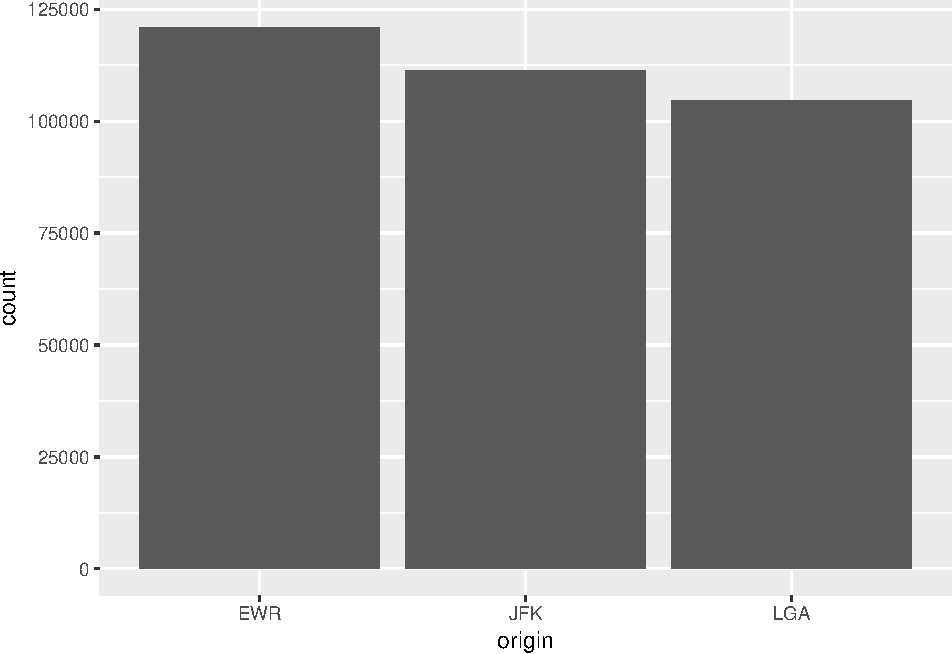
\includegraphics{01-Introduction_files/figure-latex/unnamed-chunk-14-1.pdf}

We can make the plot more informative and aesthetic.

\begin{Shaded}
\begin{Highlighting}[]
\KeywordTok{ggplot}\NormalTok{(}\DataTypeTok{data =} \NormalTok{flights, }
       \DataTypeTok{mapping =} \KeywordTok{aes}\NormalTok{(}\DataTypeTok{x =} \NormalTok{origin, }\DataTypeTok{fill =} \NormalTok{origin)) +}\StringTok{  }\CommentTok{# here "fill" gives bars distinct colors }
\StringTok{  }\KeywordTok{geom_bar}\NormalTok{() +}\StringTok{  }
\StringTok{  }\KeywordTok{facet_wrap}\NormalTok{( ~}\StringTok{ }\NormalTok{hour)  }\CommentTok{#  "facet_wrap( ~ var)" generates a grid of plots by var }
\end{Highlighting}
\end{Shaded}

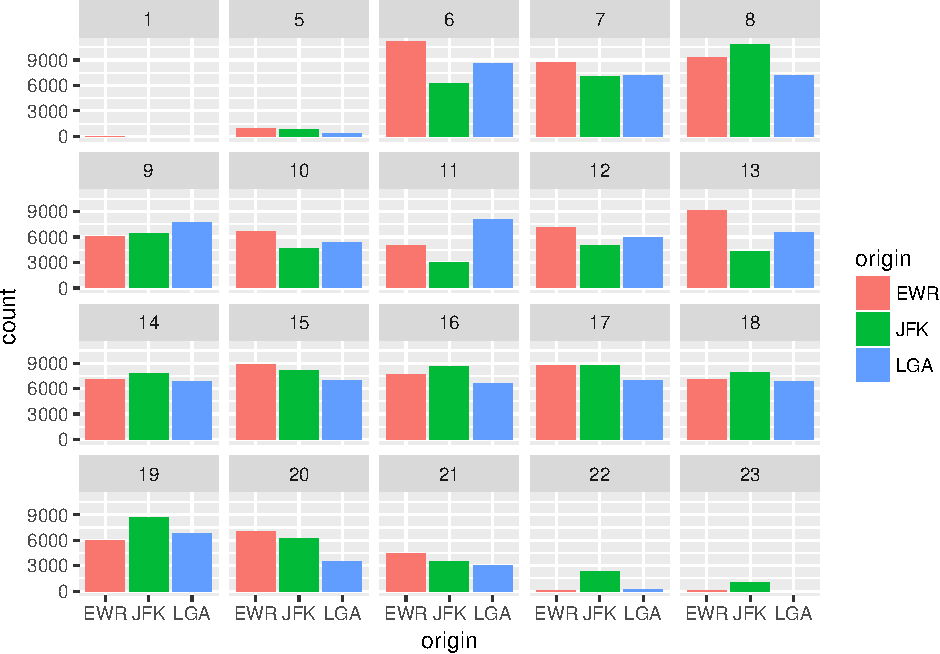
\includegraphics{01-Introduction_files/figure-latex/unnamed-chunk-15-1.pdf}

Another way to see the same information is a \textbf{histogram}.

\begin{Shaded}
\begin{Highlighting}[]
\NormalTok{flights %>%}\StringTok{ }
\StringTok{  }\KeywordTok{filter}\NormalTok{(hour >=}\StringTok{ }\DecValTok{5}\NormalTok{) %>%}\StringTok{  }\CommentTok{# exclude hour earlier than 5 a.m.}
\StringTok{  }\KeywordTok{ggplot}\NormalTok{(}\KeywordTok{aes}\NormalTok{(}\DataTypeTok{x =} \NormalTok{hour, }\DataTypeTok{fill =} \NormalTok{origin)) +}\StringTok{ }\KeywordTok{geom_histogram}\NormalTok{(}\DataTypeTok{binwidth =} \DecValTok{1}\NormalTok{, }\DataTypeTok{color =} \StringTok{"white"}\NormalTok{) }
\end{Highlighting}
\end{Shaded}

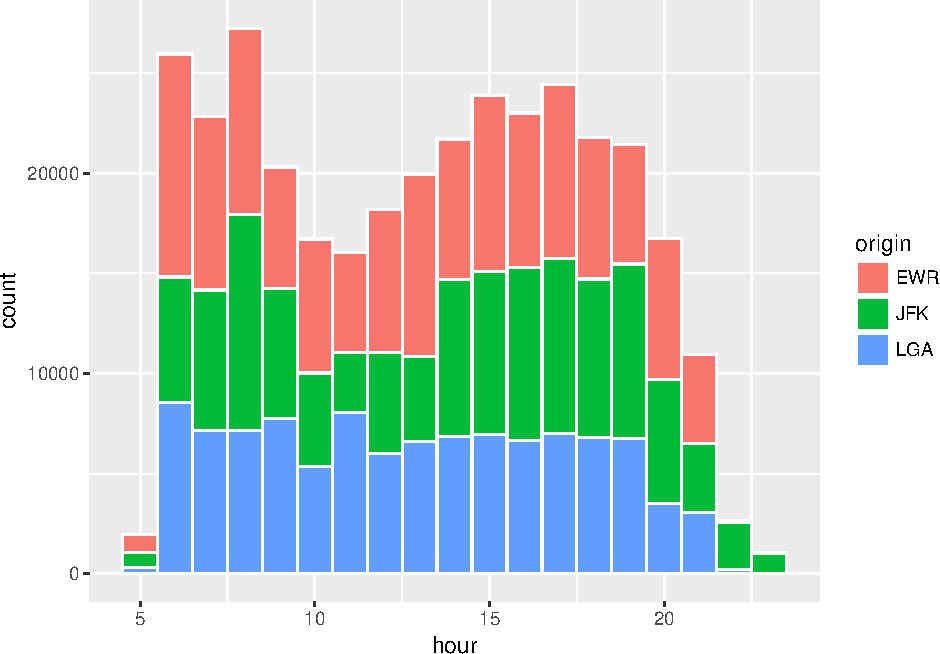
\includegraphics{01-Introduction_files/figure-latex/unnamed-chunk-16-1.pdf}

While mornings and late afternoons tend to get busy, there is not much
difference in the number of flights across airports.

Let's see if there are distinct patters of departure delays over the
course of a year. We do this by taking the average of departure delays
for each day by flight origin and plot the data as a time series using
\textbf{line-graphs}.

\begin{Shaded}
\begin{Highlighting}[]
\NormalTok{delay_day <-}\StringTok{ }\NormalTok{flights %>%}\StringTok{ }
\StringTok{  }\KeywordTok{group_by}\NormalTok{(origin, year, month, day) %>%}\StringTok{ }
\StringTok{  }\KeywordTok{summarise}\NormalTok{(}\DataTypeTok{dep_delay =} \KeywordTok{mean}\NormalTok{(dep_delay, }\DataTypeTok{na.rm =} \OtherTok{TRUE}\NormalTok{))  %>%}\StringTok{ }
\StringTok{  }\KeywordTok{mutate}\NormalTok{(}\DataTypeTok{date =} \KeywordTok{as.Date}\NormalTok{(}\KeywordTok{paste}\NormalTok{(year, month, day), }\DataTypeTok{format=}\StringTok{"%Y %m %d"}\NormalTok{)) %>%}
\StringTok{ }\KeywordTok{filter}\NormalTok{(!}\KeywordTok{is.na}\NormalTok{(dep_delay))  }\CommentTok{#  exclude rows with dep_delay == NA }

\NormalTok{delay_day %>%}\StringTok{     }\CommentTok{# "facet_grid( var ~ .)" is similar to "facet_wrap( ~ var)" }
\StringTok{  }\KeywordTok{ggplot}\NormalTok{(}\KeywordTok{aes}\NormalTok{(}\DataTypeTok{x =} \NormalTok{date, }\DataTypeTok{y =} \NormalTok{dep_delay)) +}\StringTok{ }\KeywordTok{geom_line}\NormalTok{() +}\StringTok{ }\KeywordTok{facet_grid}\NormalTok{( origin ~}\StringTok{ }\NormalTok{. ) }
\end{Highlighting}
\end{Shaded}

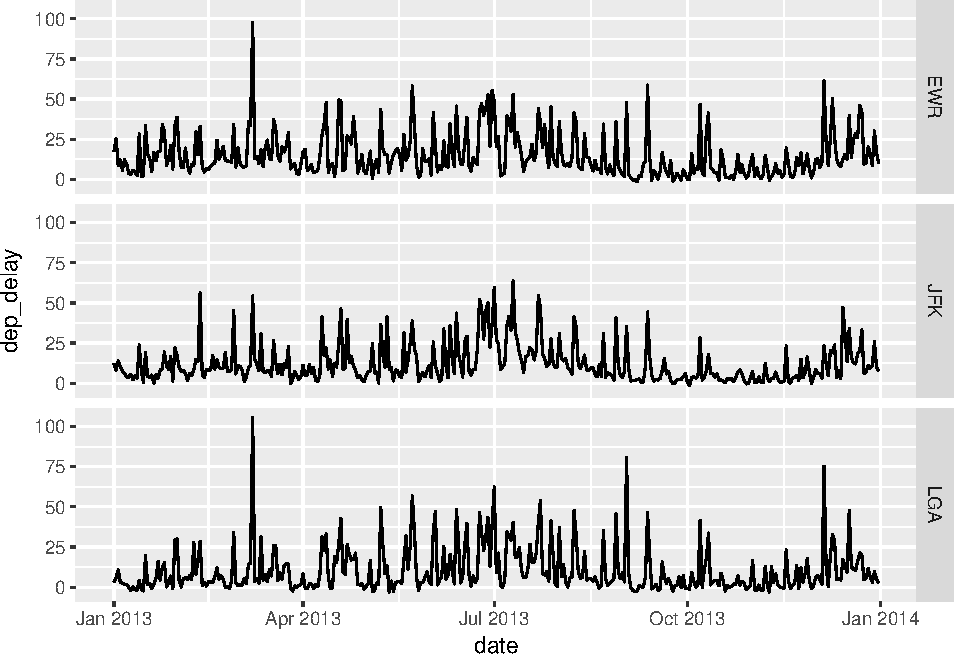
\includegraphics{01-Introduction_files/figure-latex/unnamed-chunk-17-1.pdf}

The seasonal pattern seems similar across airports, and summer months
appear to be busier on average. Let's see how closely these patterns
across airports are related to each other by focusing on a few summer
months and overlying the line-graphs.

\begin{Shaded}
\begin{Highlighting}[]
\NormalTok{delay_day %>%}\StringTok{ }
\StringTok{  }\KeywordTok{filter}\NormalTok{(}\StringTok{"2013-07-01"} \NormalTok{<=}\StringTok{ }\NormalTok{date, }\StringTok{"2013-08-31"} \NormalTok{>=}\StringTok{ }\NormalTok{date)  %>%}\StringTok{ }
\StringTok{  }\KeywordTok{ggplot}\NormalTok{(}\KeywordTok{aes}\NormalTok{(}\DataTypeTok{x =} \NormalTok{date, }\DataTypeTok{y =} \NormalTok{dep_delay, }\DataTypeTok{color =} \NormalTok{origin)) +}\StringTok{ }\KeywordTok{geom_line}\NormalTok{()  }
\end{Highlighting}
\end{Shaded}

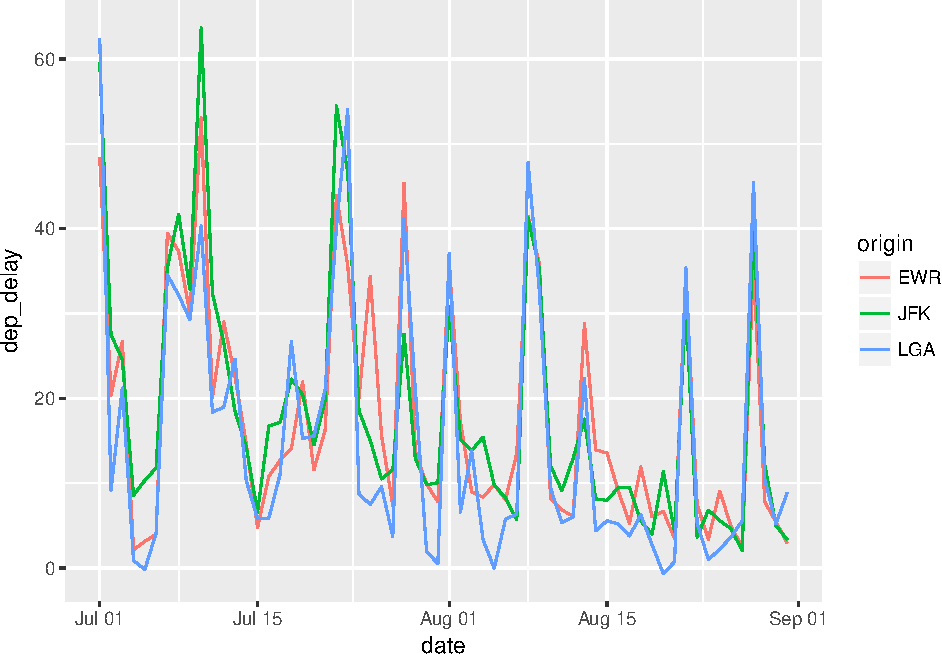
\includegraphics{01-Introduction_files/figure-latex/unnamed-chunk-18-1.pdf}

We can see similar patterns of spikes across airports occurring on
certain days, indicating a tendency that the three airports get busy on
the same days. Would this mean that the three airports tend to be
congested at the same time?

In the previous figure, there seems to be some cyclical pattern of
delays. A good place to start would be comparing delays by day of the
week. Here is a function to calculate day of the week for a given date.

\begin{Shaded}
\begin{Highlighting}[]
\NormalTok{my_dow <-}\StringTok{ }\NormalTok{function(date) \{}
  \CommentTok{# as.POSIXlt(date)[['wday']] returns integers 0, 1, 2, .. 6, for Sun, Mon, ... Sat.  }
  \CommentTok{# We extract one item from a vector (Sun, Mon, ..., Sat) by position numbered from 1 to 7. }
  \NormalTok{dow <-}\StringTok{ }\KeywordTok{as.POSIXlt}\NormalTok{(date)[[}\StringTok{'wday'}\NormalTok{]] +}\StringTok{ }\DecValTok{1}
  \KeywordTok{c}\NormalTok{(}\StringTok{"Sun"}\NormalTok{, }\StringTok{"Mon"}\NormalTok{, }\StringTok{"Tue"}\NormalTok{, }\StringTok{"Wed"}\NormalTok{, }\StringTok{"Thu"}\NormalTok{, }\StringTok{"Fri"}\NormalTok{, }\StringTok{"Sat"}\NormalTok{)[dow]  }\CommentTok{# extract "dow"-th element    }
\NormalTok{\} }
  \CommentTok{# Input: date in the format as in "2017-01-23"}
  \CommentTok{# Output: day of week }
\KeywordTok{Sys.Date}\NormalTok{()  }\CommentTok{# Sys.Date() returns the current date }
\end{Highlighting}
\end{Shaded}

\begin{verbatim}
## [1] "2017-04-08"
\end{verbatim}

\begin{Shaded}
\begin{Highlighting}[]
\KeywordTok{my_dow}\NormalTok{(}\KeywordTok{Sys.Date}\NormalTok{()) }
\end{Highlighting}
\end{Shaded}

\begin{verbatim}
## [1] "Sat"
\end{verbatim}

Now, let's take a look at the mean delay by day of the week using
\textbf{boxplots}.

\begin{Shaded}
\begin{Highlighting}[]
\NormalTok{delay_day <-}\StringTok{ }\NormalTok{flights %>%}\StringTok{ }
\StringTok{  }\KeywordTok{group_by}\NormalTok{(year, month, day) %>%}\StringTok{ }
\StringTok{  }\KeywordTok{summarise}\NormalTok{(}\DataTypeTok{dep_delay =} \KeywordTok{mean}\NormalTok{(dep_delay, }\DataTypeTok{na.rm =} \OtherTok{TRUE}\NormalTok{))  %>%}\StringTok{ }
\StringTok{  }\KeywordTok{mutate}\NormalTok{(}\DataTypeTok{date =} \KeywordTok{as.Date}\NormalTok{(}\KeywordTok{paste}\NormalTok{(year, month, day), }\DataTypeTok{format=}\StringTok{"%Y %m %d"}\NormalTok{),  }
         \CommentTok{# date defined by as.Data() function }
         \DataTypeTok{wday =} \KeywordTok{my_dow}\NormalTok{(date),}
         \DataTypeTok{weekend =} \NormalTok{wday %in%}\StringTok{ }\KeywordTok{c}\NormalTok{(}\StringTok{"Sat"}\NormalTok{, }\StringTok{"Sun"}\NormalTok{)  }
         \CommentTok{# %in% operator: A %in% B returns TRUE/FALSE for whether each element of A is in B. }
  \NormalTok{)}

\CommentTok{# show the first 10 elements of "wday" variable in "delay_day" data frame }
\NormalTok{delay_day$wday[}\DecValTok{1}\NormalTok{:}\DecValTok{10}\NormalTok{]  }
\end{Highlighting}
\end{Shaded}

\begin{verbatim}
##  [1] "Tue" "Wed" "Thu" "Fri" "Sat" "Sun" "Mon" "Tue" "Wed" "Thu"
\end{verbatim}

\begin{Shaded}
\begin{Highlighting}[]
\NormalTok{delay_day$wday <-}\StringTok{ }\KeywordTok{ordered}\NormalTok{(delay_day$wday, }
                         \DataTypeTok{levels =} \KeywordTok{c}\NormalTok{(}\StringTok{"Mon"}\NormalTok{, }\StringTok{"Tue"}\NormalTok{, }\StringTok{"Wed"}\NormalTok{, }\StringTok{"Thu"}\NormalTok{, }\StringTok{"Fri"}\NormalTok{, }\StringTok{"Sat"}\NormalTok{, }\StringTok{"Sun"}\NormalTok{))}
                            \CommentTok{# adding a sorting order (Mon, Tue, ..., Sun)   }
\NormalTok{delay_day$wday[}\DecValTok{1}\NormalTok{:}\DecValTok{10}\NormalTok{]  }
\end{Highlighting}
\end{Shaded}

\begin{verbatim}
##  [1] Tue Wed Thu Fri Sat Sun Mon Tue Wed Thu
## Levels: Mon < Tue < Wed < Thu < Fri < Sat < Sun
\end{verbatim}

\begin{Shaded}
\begin{Highlighting}[]
\NormalTok{delay_day  %>%}\StringTok{ }
\StringTok{  }\KeywordTok{filter}\NormalTok{(!}\KeywordTok{is.na}\NormalTok{(dep_delay)) %>%}
\StringTok{  }\KeywordTok{ggplot}\NormalTok{(}\KeywordTok{aes}\NormalTok{(}\DataTypeTok{x =} \NormalTok{wday, }\DataTypeTok{y =} \NormalTok{dep_delay, }\DataTypeTok{fill =} \NormalTok{weekend)) +}\StringTok{ }\KeywordTok{geom_boxplot}\NormalTok{() }
\end{Highlighting}
\end{Shaded}

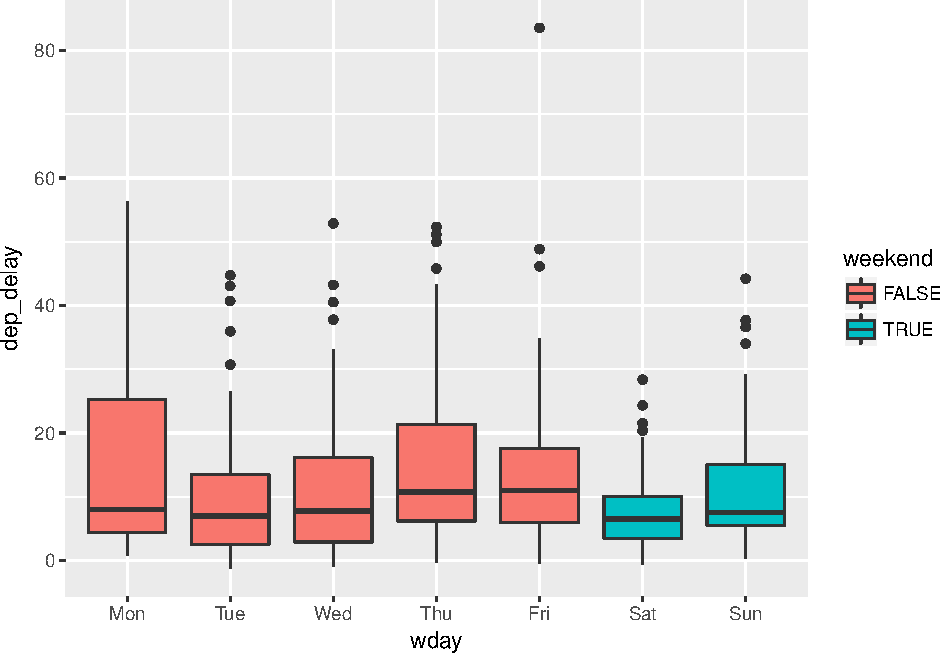
\includegraphics{01-Introduction_files/figure-latex/unnamed-chunk-20-1.pdf}

It appears that delays are on average longer on Thursdays and Fridays
and shorter on Saturdays. This is plausible if more people are traveling
on Thursdays and Fridays before the weekend, and less are traveling on
Saturdays to enjoy the weekend. Are Saturdays really less busy? Let's
find out.

\begin{Shaded}
\begin{Highlighting}[]
\NormalTok{flights_wday <-}\StringTok{ }\NormalTok{flights %>%}\StringTok{ }
\StringTok{  }\KeywordTok{mutate}\NormalTok{(}\DataTypeTok{date =} \KeywordTok{as.Date}\NormalTok{(}\KeywordTok{paste}\NormalTok{(year, month, day), }\DataTypeTok{format=}\StringTok{"%Y %m %d"}\NormalTok{),  }
         \DataTypeTok{wday =} \KeywordTok{ordered}\NormalTok{(}\KeywordTok{my_dow}\NormalTok{(date),}
                        \DataTypeTok{levels =} \KeywordTok{c}\NormalTok{(}\StringTok{"Mon"}\NormalTok{, }\StringTok{"Tue"}\NormalTok{, }\StringTok{"Wed"}\NormalTok{, }\StringTok{"Thu"}\NormalTok{, }\StringTok{"Fri"}\NormalTok{, }\StringTok{"Sat"}\NormalTok{, }\StringTok{"Sun"}\NormalTok{)),}
         \DataTypeTok{weekend =} \NormalTok{wday %in%}\StringTok{ }\KeywordTok{c}\NormalTok{(}\StringTok{"Sat"}\NormalTok{, }\StringTok{"Sun"}\NormalTok{)  }
  \NormalTok{)}

\NormalTok{flights_wday %>%}\StringTok{ }
\StringTok{  }\KeywordTok{group_by}\NormalTok{(wday) %>%}
\StringTok{  }\KeywordTok{summarise}\NormalTok{( }\DataTypeTok{nobs =} \KeywordTok{n}\NormalTok{() )}
\end{Highlighting}
\end{Shaded}

\begin{verbatim}
## # A tibble: 7 × 2
##    wday  nobs
##   <ord> <int>
## 1   Mon 50690
## 2   Tue 50422
## 3   Wed 50060
## 4   Thu 50219
## 5   Fri 50308
## 6   Sat 38720
## 7   Sun 46357
\end{verbatim}

\begin{Shaded}
\begin{Highlighting}[]
\NormalTok{flights_wday  %>%}\StringTok{ }
\StringTok{  }\KeywordTok{ggplot}\NormalTok{(}\KeywordTok{aes}\NormalTok{(}\DataTypeTok{x =} \NormalTok{wday)) +}\StringTok{ }\KeywordTok{geom_bar}\NormalTok{() }
\end{Highlighting}
\end{Shaded}

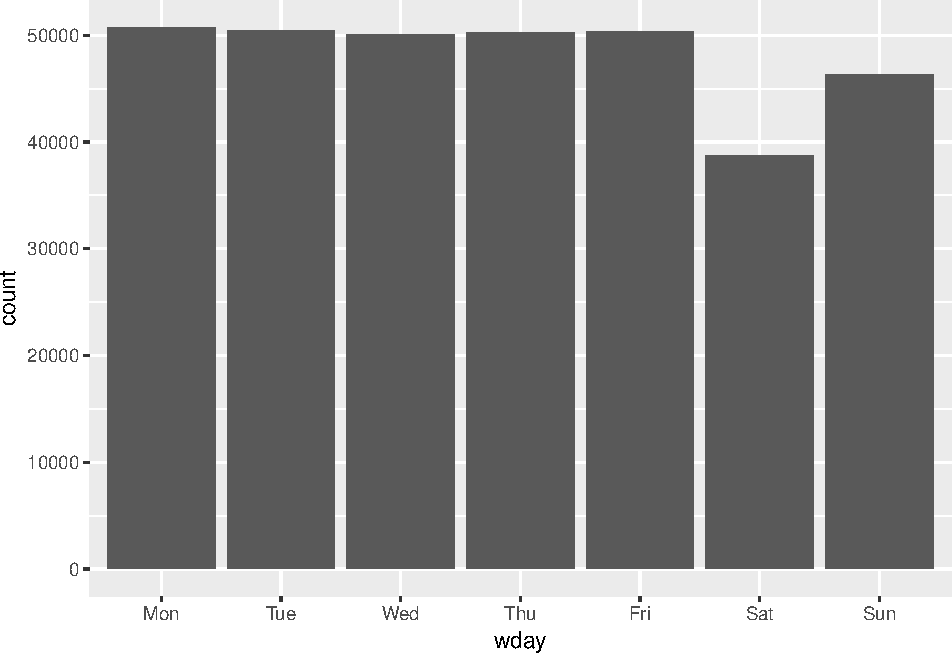
\includegraphics{01-Introduction_files/figure-latex/unnamed-chunk-21-1.pdf}

Yes, Saturdays are less busy for the airports in terms of flight
numbers.

Could we generalize this positive relationship between the number of
flights and the average delays, which we find across days of the week?
To investigate this, we can summarize the data into the average delays
by date-hour and see if the busyness of a particular hour of a
particular day is correlated with the mean delay. We visualize these
data using a \textbf{scatter plot}.

\begin{Shaded}
\begin{Highlighting}[]
\NormalTok{delay_day_hr <-}\StringTok{ }\NormalTok{flights %>%}\StringTok{ }
\StringTok{  }\KeywordTok{group_by}\NormalTok{(year, month, day, hour) %>%}\StringTok{  }\CommentTok{# grouping by date-hour }
\StringTok{  }\KeywordTok{summarise}\NormalTok{(}
    \DataTypeTok{n_obs =} \KeywordTok{n}\NormalTok{(),}
    \DataTypeTok{dep_delay =} \KeywordTok{mean}\NormalTok{(dep_delay, }\DataTypeTok{na.rm =} \OtherTok{TRUE}\NormalTok{)}
    \NormalTok{)  %>%}\StringTok{ }
\StringTok{  }\KeywordTok{mutate}\NormalTok{(}\DataTypeTok{date =} \KeywordTok{as.Date}\NormalTok{(}\KeywordTok{paste}\NormalTok{(year, month, day), }\DataTypeTok{format=}\StringTok{"%Y %m %d"}\NormalTok{),}
         \DataTypeTok{wday =} \KeywordTok{my_dow}\NormalTok{(date)}
  \NormalTok{)}

\NormalTok{plot_delay <-}\StringTok{ }\NormalTok{delay_day_hr  %>%}
\StringTok{  }\KeywordTok{filter}\NormalTok{(!}\KeywordTok{is.na}\NormalTok{(dep_delay)) %>%}\StringTok{ }
\StringTok{  }\KeywordTok{ggplot}\NormalTok{(}\KeywordTok{aes}\NormalTok{(}\DataTypeTok{x =} \NormalTok{n_obs, }\DataTypeTok{y =} \NormalTok{dep_delay)) +}\StringTok{ }\KeywordTok{geom_point}\NormalTok{(}\DataTypeTok{alpha =} \FloatTok{0.1}\NormalTok{)  }
    \CommentTok{# plot of n_obs and the average dep_delay }
    \CommentTok{# where each point represents an date-hour average}
    \CommentTok{# "alpha = 0.1"  controls the degree of transparency of points }

\NormalTok{plot_delay }
\end{Highlighting}
\end{Shaded}

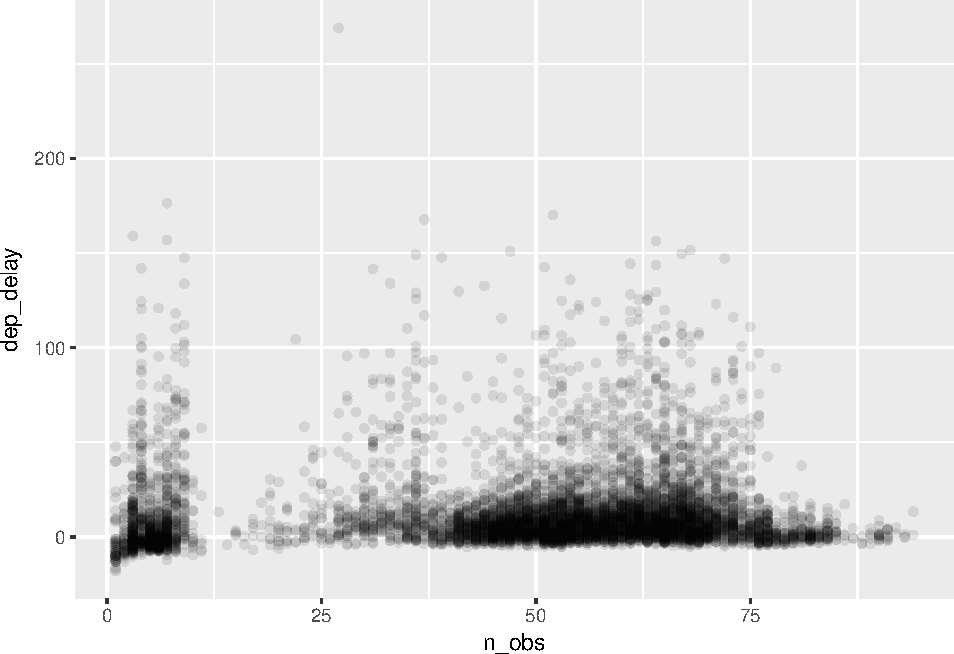
\includegraphics{01-Introduction_files/figure-latex/unnamed-chunk-22-1.pdf}

Along the horizontal axis, we can see how the number of flights is
distributed across date-hours. Some days are busy, and some hours busier
still. It appears that there are two clusters in the number of lights,
showing very slow date-hours (e.g., less than 10 flights flying out of
New York city per hour) and normal date-hours (e.g., about 50 to 70
flights per hour). We could guess that the delays in the slow hours be
caused by bad weather. On the other hand, we may wonder if the excess
delays in the normal hours, compared to the slow hours, are caused by
congestion at the airports. To see this, let's fit a curve that captures
the relationships between \texttt{n\_obs} and \texttt{dep\_delay}. Our
hypothesis is that the delay would become more likely and longer as the
number of flights increases.

\begin{Shaded}
\begin{Highlighting}[]
\NormalTok{plot_delay  +}
\StringTok{  }\KeywordTok{geom_smooth}\NormalTok{()   }\CommentTok{#  geom_smooth() addes a layer of fitted curve(s) }
\end{Highlighting}
\end{Shaded}

\begin{verbatim}
## `geom_smooth()` using method = 'gam'
\end{verbatim}

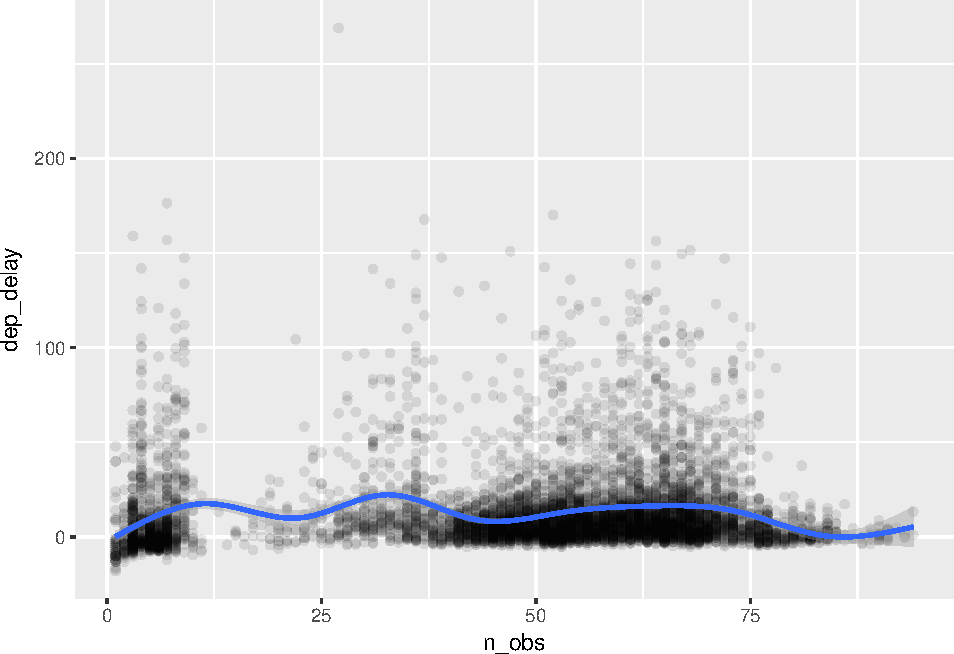
\includegraphics{01-Introduction_files/figure-latex/unnamed-chunk-23-1.pdf}

We cannot see any clear pattern. How about fitting a curve by day of the
week?

\begin{Shaded}
\begin{Highlighting}[]
\NormalTok{plot_delay  +}
\StringTok{     }\CommentTok{# additional aes() argument for applying different colors to the day of the week}
\StringTok{  }\KeywordTok{geom_smooth}\NormalTok{(}\KeywordTok{aes}\NormalTok{(}\DataTypeTok{color =} \NormalTok{wday), }\DataTypeTok{se=}\OtherTok{FALSE}\NormalTok{) }
\end{Highlighting}
\end{Shaded}

\begin{verbatim}
## `geom_smooth()` using method = 'gam'
\end{verbatim}

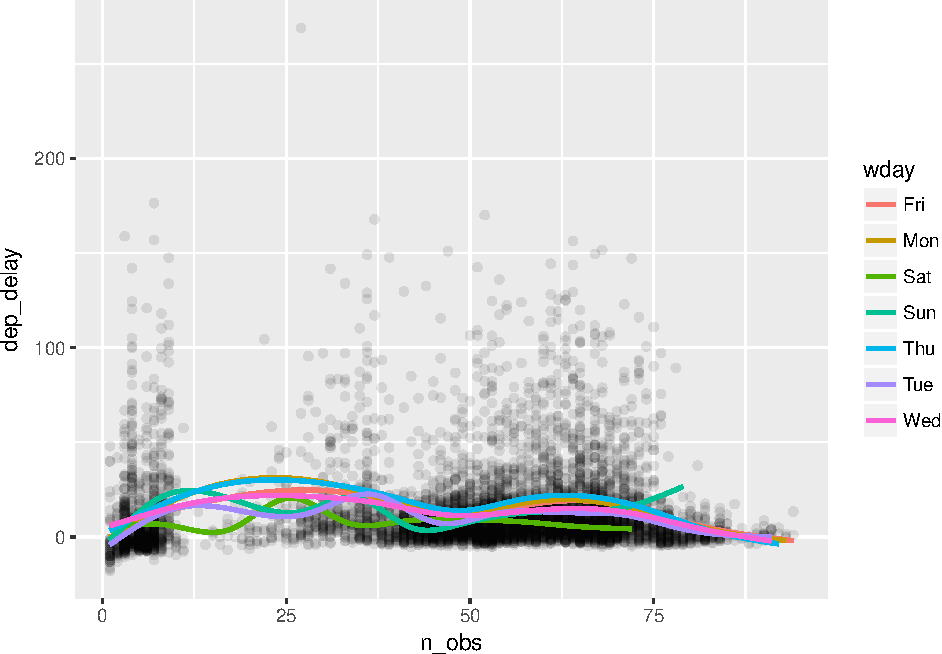
\includegraphics{01-Introduction_files/figure-latex/unnamed-chunk-24-1.pdf}

Surprisingly, the delay does not seem to increase with the flights.
There are more delays on Thursdays and Fridays and less delays on
Saturdays, but we see no evidence of congestion as a cause of delay.

Let's take a closer look at the distribution of the delays. If it is not
normally distributed, we may want to apply a transformation.

\begin{Shaded}
\begin{Highlighting}[]
\NormalTok{delay_day_hr %>%}\StringTok{  }\KeywordTok{filter}\NormalTok{(!}\KeywordTok{is.na}\NormalTok{(dep_delay)) %>%}\StringTok{ }
\StringTok{  }\KeywordTok{ggplot}\NormalTok{(}\KeywordTok{aes}\NormalTok{(}\DataTypeTok{x =} \NormalTok{dep_delay)) +}\StringTok{ }\KeywordTok{geom_histogram}\NormalTok{(}\DataTypeTok{color =} \StringTok{"white"}\NormalTok{) }
\end{Highlighting}
\end{Shaded}

\begin{verbatim}
## `stat_bin()` using `bins = 30`. Pick better value with `binwidth`.
\end{verbatim}

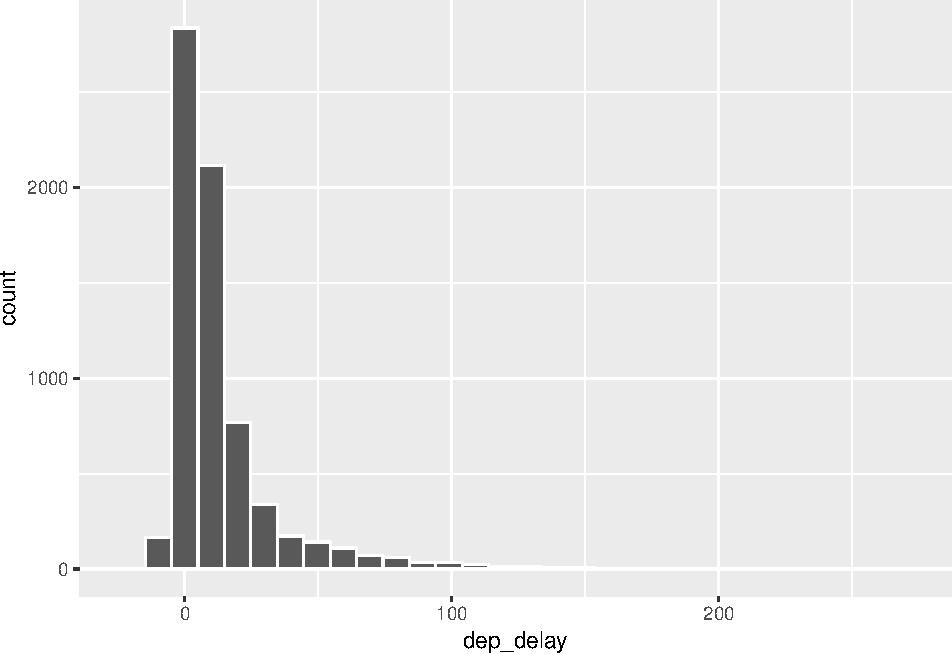
\includegraphics{01-Introduction_files/figure-latex/unnamed-chunk-25-1.pdf}

The distribution of the average delays are greatly skewed.\\
In applying a logarithmic transformation, here we have to shift the
variable so that its minimum is greater than zero.

\begin{Shaded}
\begin{Highlighting}[]
\CommentTok{# define new column called "dep_delay_shifted"}
\NormalTok{delay_day_hr$dep_delay_shifted <-}\StringTok{ }\NormalTok{delay_day_hr %>%}\StringTok{  }
\StringTok{  }\KeywordTok{with}\NormalTok{(dep_delay -}\StringTok{ }\KeywordTok{min}\NormalTok{(dep_delay, }\DataTypeTok{na.rm =} \OtherTok{TRUE}\NormalTok{) +}\StringTok{ }\DecValTok{1}\NormalTok{) }
    \CommentTok{# with() function takes a data frame in the first argument and allows for }
    \CommentTok{# referencing its variable names. }

\NormalTok{delay_day_hr %>%}\StringTok{ }
\StringTok{  }\KeywordTok{ungroup}\NormalTok{() %>%}\StringTok{   }\CommentTok{# removing group_by() attribute}
\StringTok{  }\KeywordTok{select}\NormalTok{(dep_delay, dep_delay_shifted) %>%}
\StringTok{  }\KeywordTok{with}\NormalTok{(}
    \KeywordTok{apply}\NormalTok{(., }\DecValTok{2}\NormalTok{, summary)}
    \CommentTok{# apply(data, num, fun)  applies function "fun" for each item }
    \CommentTok{# in dimension "num" (1 = cows, 2= columns) of the data frame    }
    \CommentTok{# Data referenced by "." means all variables of the dataset inside with().   }
    \NormalTok{) %>%}\StringTok{ }\KeywordTok{t}\NormalTok{() }\CommentTok{#  transpose rows and columns  }
\end{Highlighting}
\end{Shaded}

\begin{verbatim}
##                   Min. 1st Qu. Median  Mean 3rd Qu. Max. NA's
## dep_delay          -18   1.054  6.571 12.99   15.44  269   13
## dep_delay_shifted    1  20.050 25.570 31.99   34.44  288   13
\end{verbatim}

Now the transformed distribution;

\begin{Shaded}
\begin{Highlighting}[]
\CommentTok{# Under the log of 10 transformation, the distribution looks closer to a normal distribution.}
\NormalTok{delay_day_hr %>%}\StringTok{ }\KeywordTok{filter}\NormalTok{(!}\KeywordTok{is.na}\NormalTok{(dep_delay_shifted)) %>%}\StringTok{ }
\StringTok{  }\KeywordTok{ggplot}\NormalTok{(}\KeywordTok{aes}\NormalTok{(}\DataTypeTok{x =} \NormalTok{dep_delay_shifted))  +}\StringTok{  }
\StringTok{  }\KeywordTok{scale_x_log10}\NormalTok{() +}\StringTok{ }
\StringTok{  }\KeywordTok{geom_histogram}\NormalTok{(}\DataTypeTok{color =} \StringTok{"white"}\NormalTok{) }
\end{Highlighting}
\end{Shaded}

\begin{verbatim}
## `stat_bin()` using `bins = 30`. Pick better value with `binwidth`.
\end{verbatim}

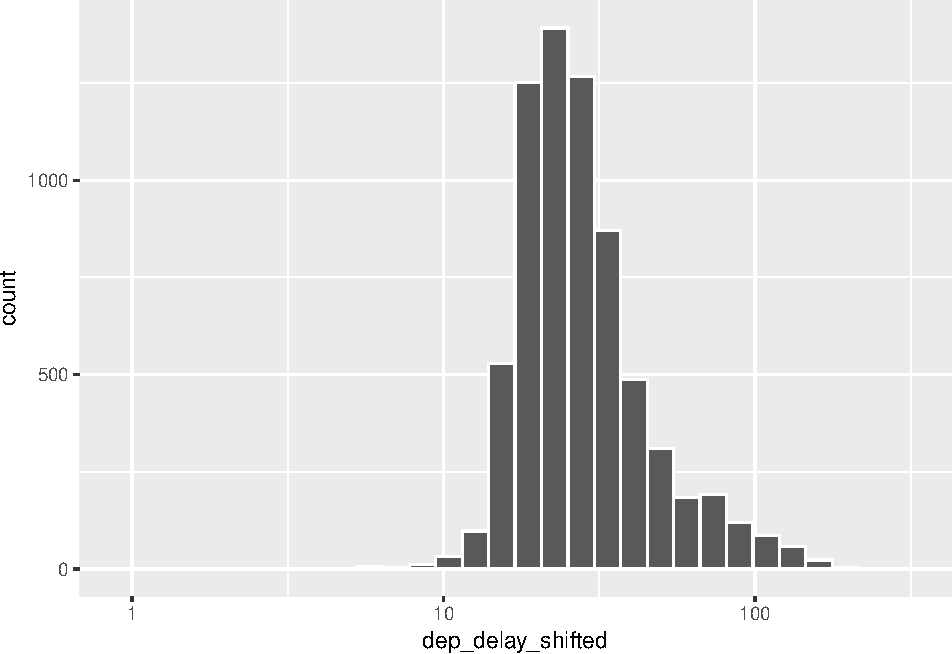
\includegraphics{01-Introduction_files/figure-latex/unnamed-chunk-27-1.pdf}

\begin{Shaded}
\begin{Highlighting}[]
\CommentTok{# Alternatively, one can apply the natural logarithm to transform a variable. Histogram shows no difference here.    }
\NormalTok{delay_day_hr %>%}\StringTok{ }\KeywordTok{filter}\NormalTok{(!}\KeywordTok{is.na}\NormalTok{(dep_delay_shifted)) %>%}\StringTok{ }
\StringTok{  }\KeywordTok{ggplot}\NormalTok{(}\KeywordTok{aes}\NormalTok{(}\DataTypeTok{x =} \NormalTok{dep_delay_shifted)) +}\StringTok{  }
\StringTok{  }\KeywordTok{scale_x_continuous}\NormalTok{(}\DataTypeTok{trans =} \StringTok{"log"}\NormalTok{) +}\StringTok{  }
\StringTok{  }\KeywordTok{geom_histogram}\NormalTok{(}\DataTypeTok{color =} \StringTok{"white"}\NormalTok{)}
\end{Highlighting}
\end{Shaded}

\begin{verbatim}
## `stat_bin()` using `bins = 30`. Pick better value with `binwidth`.
\end{verbatim}

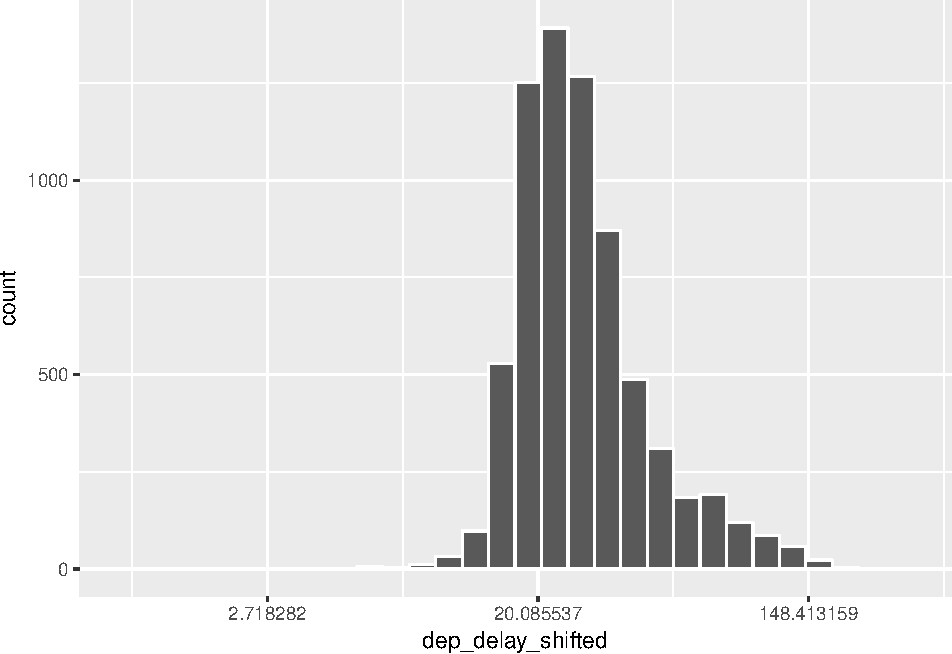
\includegraphics{01-Introduction_files/figure-latex/unnamed-chunk-27-2.pdf}

The transformed distribution is much less skewed than the original. Now,
let's plot the relationship between delays and flights again.

\begin{Shaded}
\begin{Highlighting}[]
\NormalTok{delay_day_hr  %>%}\StringTok{ }\KeywordTok{filter}\NormalTok{(!}\KeywordTok{is.na}\NormalTok{(dep_delay_shifted), dep_delay_shifted >}\StringTok{ }\DecValTok{5}\NormalTok{) %>%}\StringTok{ }
\StringTok{  }\KeywordTok{ggplot}\NormalTok{(}\KeywordTok{aes}\NormalTok{(}\DataTypeTok{x =} \NormalTok{n_obs, }\DataTypeTok{y =} \NormalTok{dep_delay_shifted)) +}\StringTok{ }
\StringTok{  }\KeywordTok{scale_y_log10}\NormalTok{() +}\StringTok{     }\CommentTok{# using transformation scale_y_log10() }
\StringTok{  }\KeywordTok{geom_point}\NormalTok{(}\DataTypeTok{alpha =} \FloatTok{0.1}\NormalTok{)  +}\StringTok{ }
\StringTok{  }\KeywordTok{geom_smooth}\NormalTok{()  }
\end{Highlighting}
\end{Shaded}

\begin{verbatim}
## `geom_smooth()` using method = 'gam'
\end{verbatim}

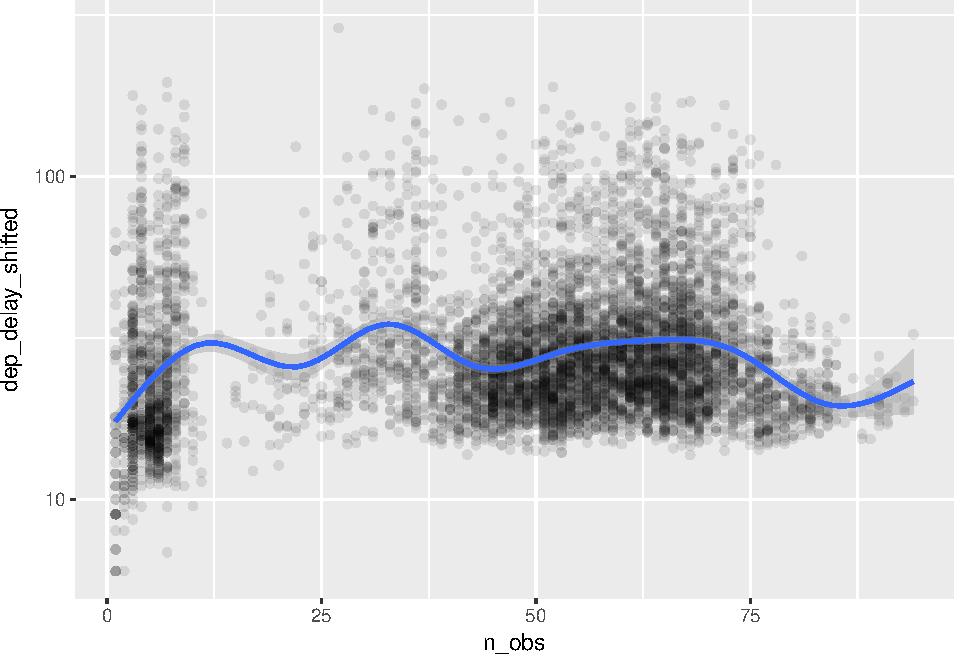
\includegraphics{01-Introduction_files/figure-latex/unnamed-chunk-28-1.pdf}

We still do not see a pattern that busier hours have more delays. This
seems to suggest that the airports in New York City manage the
fluctuating number of flights without causing congestion.

\section{Huning down numbers}\label{huning-down-numbers}

This section is optional but contains more examples of \texttt{dplyr}
and \texttt{ggplot2} functions.

Previously, we find that the congestion at the airports is unlikely the
cause of delays. Then, what else may explain the patterns of delays? Are
the airlines partly responsible? Recall that earlier we observe that
some airlines have longer delays than others for NYC-MSP flights. Let's
take a look at the overall average delays by carrier.

\begin{Shaded}
\begin{Highlighting}[]
\NormalTok{stat_carrier <-}\StringTok{ }\NormalTok{flights %>%}\StringTok{ }
\StringTok{  }\KeywordTok{group_by}\NormalTok{(carrier) %>%}
\StringTok{  }\KeywordTok{summarise}\NormalTok{(}\DataTypeTok{n_obs =} \KeywordTok{n}\NormalTok{(),}
            \DataTypeTok{dep_delay =} \KeywordTok{mean}\NormalTok{(dep_delay, }\DataTypeTok{na.rm =} \OtherTok{TRUE}\NormalTok{),}
            \DataTypeTok{arr_delay =} \KeywordTok{mean}\NormalTok{(arr_delay, }\DataTypeTok{na.rm =} \OtherTok{TRUE}\NormalTok{)}
            \NormalTok{) %>%}\StringTok{ }
\StringTok{  }\KeywordTok{left_join}\NormalTok{(airlines, }\DataTypeTok{by=}\StringTok{"carrier"}\NormalTok{) %>%}
\StringTok{  }\KeywordTok{arrange}\NormalTok{(}\KeywordTok{desc}\NormalTok{(n_obs)) }

\NormalTok{stat_carrier %>%}\StringTok{ }\KeywordTok{kable}\NormalTok{(}\DataTypeTok{digit=}\DecValTok{2}\NormalTok{)}
\end{Highlighting}
\end{Shaded}

\begin{tabular}{l|r|r|r|l}
\hline
carrier & n\_obs & dep\_delay & arr\_delay & name\\
\hline
UA & 58665 & 12.11 & 3.56 & United Air Lines Inc.\\
\hline
B6 & 54635 & 13.02 & 9.46 & JetBlue Airways\\
\hline
EV & 54173 & 19.96 & 15.80 & ExpressJet Airlines Inc.\\
\hline
DL & 48110 & 9.26 & 1.64 & Delta Air Lines Inc.\\
\hline
AA & 32729 & 8.59 & 0.36 & American Airlines Inc.\\
\hline
MQ & 26397 & 10.55 & 10.77 & Envoy Air\\
\hline
US & 20536 & 3.78 & 2.13 & US Airways Inc.\\
\hline
9E & 18460 & 16.73 & 7.38 & Endeavor Air Inc.\\
\hline
WN & 12275 & 17.71 & 9.65 & Southwest Airlines Co.\\
\hline
VX & 5162 & 12.87 & 1.76 & Virgin America\\
\hline
FL & 3260 & 18.73 & 20.12 & AirTran Airways Corporation\\
\hline
AS & 714 & 5.80 & -9.93 & Alaska Airlines Inc.\\
\hline
F9 & 685 & 20.22 & 21.92 & Frontier Airlines Inc.\\
\hline
YV & 601 & 19.00 & 15.56 & Mesa Airlines Inc.\\
\hline
HA & 342 & 4.90 & -6.92 & Hawaiian Airlines Inc.\\
\hline
OO & 32 & 12.59 & 11.93 & SkyWest Airlines Inc.\\
\hline
\end{tabular}

There could be some differences across carriers. However, the simple
average of delays across various routes, days, and hours of flights may
not be a good measure to compare the carriers. For example, some
carriers may serve the routes and hours that tend to have more delays.
Also, given that our dataset covers only the flights from New York City,
the comparison may not be nationally representative since carriers use
different airports around the country for their regional hubs.

For our purposes, let's compare the average air time among carriers,
while accounting for flight's destination and timing. The differences in
air time are not the same as the differences in delays, but they may
indicate some efficiency difference among carriers.

Let's first check how air time relates to flight distance.

\begin{Shaded}
\begin{Highlighting}[]
\NormalTok{flights %>%}\StringTok{ }
\StringTok{  }\KeywordTok{filter} \NormalTok{(month ==}\StringTok{ }\DecValTok{1}\NormalTok{, day ==}\StringTok{ }\DecValTok{1}\NormalTok{, !}\KeywordTok{is.na}\NormalTok{(air_time)) %>%}
\StringTok{  }\KeywordTok{ggplot}\NormalTok{(}\KeywordTok{aes}\NormalTok{(}\DataTypeTok{x =} \NormalTok{distance, }\DataTypeTok{y =} \NormalTok{air_time)) +}\StringTok{ }
\StringTok{  }\KeywordTok{geom_point}\NormalTok{(}\DataTypeTok{alpha =} \FloatTok{0.05}\NormalTok{)  +}\StringTok{  }
\StringTok{  }\KeywordTok{geom_smooth}\NormalTok{()}
\end{Highlighting}
\end{Shaded}

\begin{verbatim}
## `geom_smooth()` using method = 'loess'
\end{verbatim}

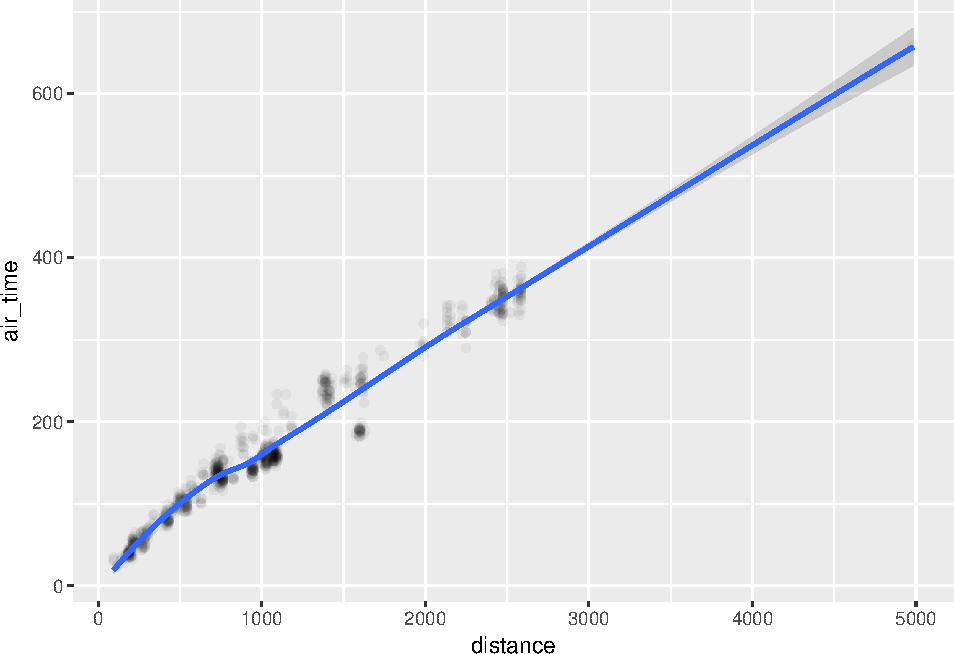
\includegraphics{01-Introduction_files/figure-latex/unnamed-chunk-30-1.pdf}

\texttt{air\_time} and \texttt{distance} shows a general linear
relationship. We can better account for this relationship if we
calculate the average air time for each flight destination from New York
City.

First, we will consider a simple approach to control for such average
air time for each destination and compare the variation in air time
among carriers. We can do this by fitting a linear regression model with
fixed destination effects and comparing the residuals. This resembles
the ANOVA for comparing the mean air times among carriers, but the fixed
destination effects here difference out the average air time for each
destination from the total variation.

\begin{Shaded}
\begin{Highlighting}[]
\CommentTok{# a copy of flights data}
\NormalTok{flights2 <-}\StringTok{ }\NormalTok{flights}

\CommentTok{# TRUE/FALSE vector showing whther air_time is not NA. }
\NormalTok{idx0 <-}\StringTok{ }\NormalTok{flights %>%}\StringTok{ }\KeywordTok{with}\NormalTok{(!}\KeywordTok{is.na}\NormalTok{(air_time))  }

\NormalTok{flights2$res <-}\StringTok{ }\OtherTok{NA} \CommentTok{# prepare a column of residuals to be defined below }

\NormalTok{flights2$res[idx0] <-}\StringTok{ }\NormalTok{flights2 %>%}\StringTok{  }\CommentTok{# replace rows with idx0 = TRUE}
\StringTok{  }\KeywordTok{filter}\NormalTok{(!}\KeywordTok{is.na}\NormalTok{(air_time)) %>%}\StringTok{ }
\StringTok{  }\KeywordTok{with}\NormalTok{( }
   \KeywordTok{lm}\NormalTok{( air_time ~}\StringTok{ }\KeywordTok{as.factor}\NormalTok{(dest))  }
        \CommentTok{# lm() estimates a linear model. }
        \CommentTok{# "y ~ x"" is the formula for regressing y on x. }
        \CommentTok{# as.factor() converts "dest" to a factor (categorical) class}
        \CommentTok{# which is used as a set of dummy variables in the regression.  }
   \NormalTok{) %>%}\StringTok{ }
\StringTok{  }\KeywordTok{residuals}\NormalTok{()  }\CommentTok{# obtains residuals of the lm() object }

\NormalTok{stat_res <-}\StringTok{ }\NormalTok{flights2 %>%}\StringTok{ }
\StringTok{  }\KeywordTok{group_by}\NormalTok{(carrier) %>%}
\StringTok{  }\KeywordTok{summarise}\NormalTok{(}
    \DataTypeTok{mean_res =} \KeywordTok{mean}\NormalTok{(res, }\DataTypeTok{na.rm =} \OtherTok{TRUE}\NormalTok{), }\CommentTok{# mean residual by carrier }
    \DataTypeTok{sd_res =} \KeywordTok{sd}\NormalTok{(res, }\DataTypeTok{na.rm =} \OtherTok{TRUE}\NormalTok{)}
    \NormalTok{) }

\KeywordTok{left_join}\NormalTok{(stat_carrier, stat_res, }\DataTypeTok{by=}\StringTok{"carrier"}\NormalTok{) %>%}\StringTok{ }\KeywordTok{kable}\NormalTok{(}\DataTypeTok{digit=}\DecValTok{2}\NormalTok{)}
\end{Highlighting}
\end{Shaded}

\begin{tabular}{l|r|r|r|l|r|r}
\hline
carrier & n\_obs & dep\_delay & arr\_delay & name & mean\_res & sd\_res\\
\hline
UA & 58665 & 12.11 & 3.56 & United Air Lines Inc. & -0.87 & 14.59\\
\hline
B6 & 54635 & 13.02 & 9.46 & JetBlue Airways & 0.28 & 11.55\\
\hline
EV & 54173 & 19.96 & 15.80 & ExpressJet Airlines Inc. & -0.37 & 8.94\\
\hline
DL & 48110 & 9.26 & 1.64 & Delta Air Lines Inc. & -0.20 & 12.32\\
\hline
AA & 32729 & 8.59 & 0.36 & American Airlines Inc. & 0.68 & 13.86\\
\hline
MQ & 26397 & 10.55 & 10.77 & Envoy Air & 0.45 & 8.87\\
\hline
US & 20536 & 3.78 & 2.13 & US Airways Inc. & -0.42 & 9.43\\
\hline
9E & 18460 & 16.73 & 7.38 & Endeavor Air Inc. & 0.84 & 8.76\\
\hline
WN & 12275 & 17.71 & 9.65 & Southwest Airlines Co. & 0.16 & 12.55\\
\hline
VX & 5162 & 12.87 & 1.76 & Virgin America & 3.26 & 17.58\\
\hline
FL & 3260 & 18.73 & 20.12 & AirTran Airways Corporation & 1.16 & 8.75\\
\hline
AS & 714 & 5.80 & -9.93 & Alaska Airlines Inc. & -2.13 & 16.17\\
\hline
F9 & 685 & 20.22 & 21.92 & Frontier Airlines Inc. & 3.12 & 15.16\\
\hline
YV & 601 & 19.00 & 15.56 & Mesa Airlines Inc. & -0.05 & 7.06\\
\hline
HA & 342 & 4.90 & -6.92 & Hawaiian Airlines Inc. & 5.64 & 20.69\\
\hline
OO & 32 & 12.59 & 11.93 & SkyWest Airlines Inc. & 1.02 & 7.26\\
\hline
\end{tabular}

The differences in air time across carriers (``mean\_res'') somewhat
differ from the patterns of differences in the simple averages of delays
(``dep\_delay'' and ``arr\_delay''). The patterns are different between
``dep\_delay'' and ``arr\_delay'' for that matter.

To some extent, it appears to make sense that the average air time is
longer for low-cost carriers such as Virgin America, Frontier Airlines,
and Hawaiian Airlines. The differences across other carriers, on the
other hand, are small, compared to the standard deviations. To get a
sense of whether these differences have any statistical significance,
let's use t-test to compare the mean residual between United Airlines
and American Airlines.

\begin{Shaded}
\begin{Highlighting}[]
\CommentTok{# t-test comparing UA vs AA for the mean air time }
\NormalTok{flights2 %>%}
\StringTok{  }\KeywordTok{with}\NormalTok{(\{}
    \NormalTok{idx_UA <-}\StringTok{ }\NormalTok{carrier ==}\StringTok{ "UA"}
    \NormalTok{idx_AA <-}\StringTok{ }\NormalTok{carrier ==}\StringTok{ "AA"}
    \KeywordTok{t.test}\NormalTok{(res[idx_UA], res[idx_AA])}
    \NormalTok{\})}
\end{Highlighting}
\end{Shaded}

\begin{verbatim}
## 
##  Welch Two Sample t-test
## 
## data:  res[idx_UA] and res[idx_AA]
## t = -15.722, df = 68826, p-value < 2.2e-16
## alternative hypothesis: true difference in means is not equal to 0
## 95 percent confidence interval:
##  -1.741133 -1.355142
## sample estimates:
##  mean of x  mean of y 
## -0.8689523  0.6791852
\end{verbatim}

With a large number of observations, a seemingly-small difference in the
means often turn out to be a statistically significant difference.
Nonetheless, statistical significance is not sufficient for being an
empirically significant difference that matters in the real world. The
average difference of about 1.5 minute air time per flight appears very
small.

In fact, we can do this sort of pair-wise comparisons all at once using
a regression. Using carrier fixed effects in addition to destination
fixed effects, we can directly compare the mean effects across carriers.
We will set United Airlines to be a reference of the carrier fixed
effects, so that the fixed effect for United Airlines is set to zero
(i.e., omitted category), from which the fixed effects of all other
airlines are estimated.

\begin{Shaded}
\begin{Highlighting}[]
\NormalTok{flights2$carrier <-}\StringTok{ }\KeywordTok{relevel}\NormalTok{(}\KeywordTok{factor}\NormalTok{(flights2$carrier), }\DataTypeTok{ref=}\StringTok{"UA"}\NormalTok{)  }
\CommentTok{# reference level is United Airlines}
\NormalTok{flights2$carrier %>%}\StringTok{ }\KeywordTok{table}\NormalTok{()}
\end{Highlighting}
\end{Shaded}

\begin{verbatim}
## .
##    UA    9E    AA    AS    B6    DL    EV    F9    FL    HA    MQ    OO 
## 58665 18460 32729   714 54635 48110 54173   685  3260   342 26397    32 
##    US    VX    WN    YV 
## 20536  5162 12275   601
\end{verbatim}

\begin{Shaded}
\begin{Highlighting}[]
\NormalTok{flights2 %>%}\StringTok{ }
\StringTok{  }\KeywordTok{with}\NormalTok{(\{}
    \NormalTok{n_carrier <-}\StringTok{ }\KeywordTok{unique}\NormalTok{(carrier) %>%}\StringTok{ }\KeywordTok{length}\NormalTok{()}
    \NormalTok{n_dest <-}\StringTok{ }\KeywordTok{unique}\NormalTok{(dest) %>%}\StringTok{ }\KeywordTok{length}\NormalTok{() }
    \KeywordTok{print}\NormalTok{(}\KeywordTok{paste}\NormalTok{(}\StringTok{'There are'}\NormalTok{, n_carrier, }\StringTok{'distinct carriers and'}\NormalTok{, }
                \NormalTok{n_dest,}\StringTok{'distinct destinations in the data.'} \NormalTok{))}
  \NormalTok{\})}
\end{Highlighting}
\end{Shaded}

\begin{verbatim}
## [1] "There are 16 distinct carriers and 105 distinct destinations in the data."
\end{verbatim}

With 16 carriers and 105 destinations minus 2 reference levels for
carriers and destinations, the total of 119 coefficients will be
estimated for the fixed effects.

\begin{Shaded}
\begin{Highlighting}[]
\NormalTok{f1 <-}\StringTok{ }\NormalTok{flights2 %>%}
\StringTok{ }\KeywordTok{with}\NormalTok{(}
   \KeywordTok{lm}\NormalTok{( air_time  ~}\StringTok{  }\KeywordTok{as.factor}\NormalTok{(carrier) +}\StringTok{ }\KeywordTok{as.factor}\NormalTok{(dest) )  }
    \CommentTok{# fixed effects for carriers and destinations}
 \NormalTok{)}

\KeywordTok{tidy}\NormalTok{(f1)[}\DecValTok{1}\NormalTok{:}\DecValTok{20}\NormalTok{,] }\CommentTok{# show the first 20 coefficients}
\end{Highlighting}
\end{Shaded}

\begin{verbatim}
##                    term     estimate  std.error    statistic       p.value
## 1           (Intercept)  247.9884874 0.75069658  330.3445016  0.000000e+00
## 2  as.factor(carrier)9E    1.8015498 0.12723996   14.1586788  1.702649e-45
## 3  as.factor(carrier)AA    1.9326712 0.09731105   19.8607572  1.002388e-87
## 4  as.factor(carrier)AS   -1.9071536 0.49596319   -3.8453531  1.204017e-04
## 5  as.factor(carrier)B6    1.1808039 0.08495098   13.8998267  6.535025e-44
## 6  as.factor(carrier)DL    0.7531812 0.08722600    8.6348244  5.907432e-18
## 7  as.factor(carrier)EV    0.4174574 0.11044837    3.7796605  1.570702e-04
## 8  as.factor(carrier)F9    3.8891981 0.48090201    8.0872985  6.120836e-16
## 9  as.factor(carrier)FL    2.6434074 0.27600661    9.5773336  1.002386e-21
## 10 as.factor(carrier)HA   11.0125104 0.89821710   12.2604106  1.503557e-34
## 11 as.factor(carrier)MQ    1.4592669 0.11892133   12.2708590  1.321669e-34
## 12 as.factor(carrier)OO    1.8091432 2.21222472    0.8177936  4.134757e-01
## 13 as.factor(carrier)US    0.1319337 0.13826299    0.9542230  3.399715e-01
## 14 as.factor(carrier)VX    4.5298528 0.18441295   24.5636378 4.086448e-133
## 15 as.factor(carrier)WN    1.2226161 0.17520980    6.9780125  2.999500e-12
## 16 as.factor(carrier)YV    0.5167461 0.52737831    0.9798395  3.271661e-01
## 17   as.factor(dest)ACK -207.1011095 1.04478912 -198.2228803  0.000000e+00
## 18   as.factor(dest)ALB -216.6188634 0.95130943 -227.7059972  0.000000e+00
## 19   as.factor(dest)ANC  165.1365126 4.26930687   38.6799351  0.000000e+00
## 20   as.factor(dest)ATL -136.1282095 0.75641976 -179.9638460  0.000000e+00
\end{verbatim}

\begin{Shaded}
\begin{Highlighting}[]
\CommentTok{# a function to clean up the coefficient table above  }
\NormalTok{clean_lm_rlt <-}\StringTok{ }\NormalTok{function(f) \{}
  \CommentTok{# keep only rows for which column "term" contains "carrier"  e.g., rows 2 to 16 above}
  \NormalTok{rlt <-}\StringTok{ }\KeywordTok{tidy}\NormalTok{(f) %>%}\StringTok{ }\KeywordTok{filter}\NormalTok{(}\KeywordTok{grepl}\NormalTok{(}\StringTok{"carrier"}\NormalTok{,term)) }

  \CommentTok{# create column named carrier }
  \NormalTok{rlt <-}\StringTok{ }\NormalTok{rlt %>%}\StringTok{ }\KeywordTok{mutate}\NormalTok{(}\DataTypeTok{carrier =} \KeywordTok{gsub}\NormalTok{(}\StringTok{'as.factor}\CharTok{\textbackslash{}\textbackslash{}}\StringTok{(carrier}\CharTok{\textbackslash{}\textbackslash{}}\StringTok{)'}\NormalTok{,}\StringTok{''}\NormalTok{, term)) }

  \CommentTok{# drop column term}
  \NormalTok{rlt <-}\StringTok{ }\NormalTok{rlt %>%}\StringTok{ }\KeywordTok{select}\NormalTok{(-term)}
  
  \CommentTok{# add columns of carrier, name, and n_obs from the stat_carrier data frame}
  \NormalTok{stat_carrier %>%}\StringTok{  }
\StringTok{    }\KeywordTok{select}\NormalTok{(carrier, name, n_obs) %>%}
\StringTok{    }\KeywordTok{left_join}\NormalTok{(rlt, }\DataTypeTok{by=}\StringTok{"carrier"}\NormalTok{) }
\NormalTok{\}}

\NormalTok{lm_rlt1 <-}\StringTok{ }\KeywordTok{clean_lm_rlt}\NormalTok{(f1)}
\NormalTok{lm_rlt1 %>%}\StringTok{ }\KeywordTok{kable}\NormalTok{(}\DataTypeTok{digit=}\DecValTok{2}\NormalTok{)}
\end{Highlighting}
\end{Shaded}

\begin{tabular}{l|l|r|r|r|r|r}
\hline
carrier & name & n\_obs & estimate & std.error & statistic & p.value\\
\hline
UA & United Air Lines Inc. & 58665 & NA & NA & NA & NA\\
\hline
B6 & JetBlue Airways & 54635 & 1.18 & 0.08 & 13.90 & 0.00\\
\hline
EV & ExpressJet Airlines Inc. & 54173 & 0.42 & 0.11 & 3.78 & 0.00\\
\hline
DL & Delta Air Lines Inc. & 48110 & 0.75 & 0.09 & 8.63 & 0.00\\
\hline
AA & American Airlines Inc. & 32729 & 1.93 & 0.10 & 19.86 & 0.00\\
\hline
MQ & Envoy Air & 26397 & 1.46 & 0.12 & 12.27 & 0.00\\
\hline
US & US Airways Inc. & 20536 & 0.13 & 0.14 & 0.95 & 0.34\\
\hline
9E & Endeavor Air Inc. & 18460 & 1.80 & 0.13 & 14.16 & 0.00\\
\hline
WN & Southwest Airlines Co. & 12275 & 1.22 & 0.18 & 6.98 & 0.00\\
\hline
VX & Virgin America & 5162 & 4.53 & 0.18 & 24.56 & 0.00\\
\hline
FL & AirTran Airways Corporation & 3260 & 2.64 & 0.28 & 9.58 & 0.00\\
\hline
AS & Alaska Airlines Inc. & 714 & -1.91 & 0.50 & -3.85 & 0.00\\
\hline
F9 & Frontier Airlines Inc. & 685 & 3.89 & 0.48 & 8.09 & 0.00\\
\hline
YV & Mesa Airlines Inc. & 601 & 0.52 & 0.53 & 0.98 & 0.33\\
\hline
HA & Hawaiian Airlines Inc. & 342 & 11.01 & 0.90 & 12.26 & 0.00\\
\hline
OO & SkyWest Airlines Inc. & 32 & 1.81 & 2.21 & 0.82 & 0.41\\
\hline
\end{tabular}

The ``estimate'' column shows the mean difference in air time with
United Airlines, accounting for flight destination. The estimate tends
to be more precise (i.e., smaller standard errors) for carriers with a
larger number of observations. This time, we find that Virgin America,
Air Tran, Frontier Airlines, and Hawaiian Airlines tend to show
particularly longer air times than United Airlines.

Next, let's take a step further to account for flight timing as well. We
can do this by adding fixed effects for flight dates and hours.

\begin{Shaded}
\begin{Highlighting}[]
\NormalTok{flights2 <-}\StringTok{ }\NormalTok{flights2 %>%}
\StringTok{  }\KeywordTok{mutate}\NormalTok{( }\DataTypeTok{date_id =} \NormalTok{month*}\DecValTok{100} \NormalTok{+}\StringTok{ }\NormalTok{day )}

\NormalTok{flights2$date_id %>%}\StringTok{ }\KeywordTok{unique}\NormalTok{() %>%}\StringTok{ }\KeywordTok{length}\NormalTok{()}
\end{Highlighting}
\end{Shaded}

\begin{verbatim}
## [1] 365
\end{verbatim}

\begin{Shaded}
\begin{Highlighting}[]
\NormalTok{f2 <-}\StringTok{ }\NormalTok{flights2 %>%}
\StringTok{ }\KeywordTok{with}\NormalTok{(}
   \KeywordTok{lm}\NormalTok{( air_time ~}\StringTok{  }\KeywordTok{as.factor}\NormalTok{(carrier) +}\StringTok{ }\KeywordTok{as.factor}\NormalTok{(dest) +}
\StringTok{        }\NormalTok{+}\StringTok{ }\KeywordTok{as.factor}\NormalTok{(date_id) +}\StringTok{ }\KeywordTok{as.factor}\NormalTok{(hour) )}
 \NormalTok{)}

\NormalTok{lm_rlt2 <-}\StringTok{ }\KeywordTok{clean_lm_rlt}\NormalTok{(f2)}
\NormalTok{lm_rlt2 %>%}\StringTok{ }\KeywordTok{kable}\NormalTok{(}\DataTypeTok{digit=}\DecValTok{2}\NormalTok{)}
\end{Highlighting}
\end{Shaded}

\begin{tabular}{l|l|r|r|r|r|r}
\hline
carrier & name & n\_obs & estimate & std.error & statistic & p.value\\
\hline
UA & United Air Lines Inc. & 58665 & NA & NA & NA & NA\\
\hline
B6 & JetBlue Airways & 54635 & 1.60 & 0.07 & 22.50 & 0.00\\
\hline
EV & ExpressJet Airlines Inc. & 54173 & 0.61 & 0.09 & 6.67 & 0.00\\
\hline
DL & Delta Air Lines Inc. & 48110 & 0.95 & 0.07 & 13.03 & 0.00\\
\hline
AA & American Airlines Inc. & 32729 & 1.84 & 0.08 & 22.81 & 0.00\\
\hline
MQ & Envoy Air & 26397 & 1.45 & 0.10 & 14.70 & 0.00\\
\hline
US & US Airways Inc. & 20536 & 0.17 & 0.11 & 1.51 & 0.13\\
\hline
9E & Endeavor Air Inc. & 18460 & 1.57 & 0.11 & 14.72 & 0.00\\
\hline
WN & Southwest Airlines Co. & 12275 & 1.14 & 0.15 & 7.82 & 0.00\\
\hline
VX & Virgin America & 5162 & 4.85 & 0.15 & 31.57 & 0.00\\
\hline
FL & AirTran Airways Corporation & 3260 & 2.19 & 0.23 & 9.58 & 0.00\\
\hline
AS & Alaska Airlines Inc. & 714 & -2.55 & 0.41 & -6.21 & 0.00\\
\hline
F9 & Frontier Airlines Inc. & 685 & 3.31 & 0.40 & 8.29 & 0.00\\
\hline
YV & Mesa Airlines Inc. & 601 & 0.32 & 0.44 & 0.73 & 0.46\\
\hline
HA & Hawaiian Airlines Inc. & 342 & 11.79 & 0.75 & 15.80 & 0.00\\
\hline
OO & SkyWest Airlines Inc. & 32 & 7.63 & 1.83 & 4.17 & 0.00\\
\hline
\end{tabular}

\begin{Shaded}
\begin{Highlighting}[]
\NormalTok{lm_rlt2 %>%}\StringTok{ }\KeywordTok{filter}\NormalTok{(carrier!=}\StringTok{'UA'}\NormalTok{) %>%}
\StringTok{  }\KeywordTok{ggplot}\NormalTok{(}\KeywordTok{aes}\NormalTok{(}\DataTypeTok{x =} \NormalTok{carrier, }\DataTypeTok{y =} \NormalTok{estimate)) +}\StringTok{ }\KeywordTok{geom_col}\NormalTok{() +}
\StringTok{  }\KeywordTok{labs}\NormalTok{(}\DataTypeTok{title =} \StringTok{"Mean Air Time Compared to United Airlines"}\NormalTok{)}
\end{Highlighting}
\end{Shaded}

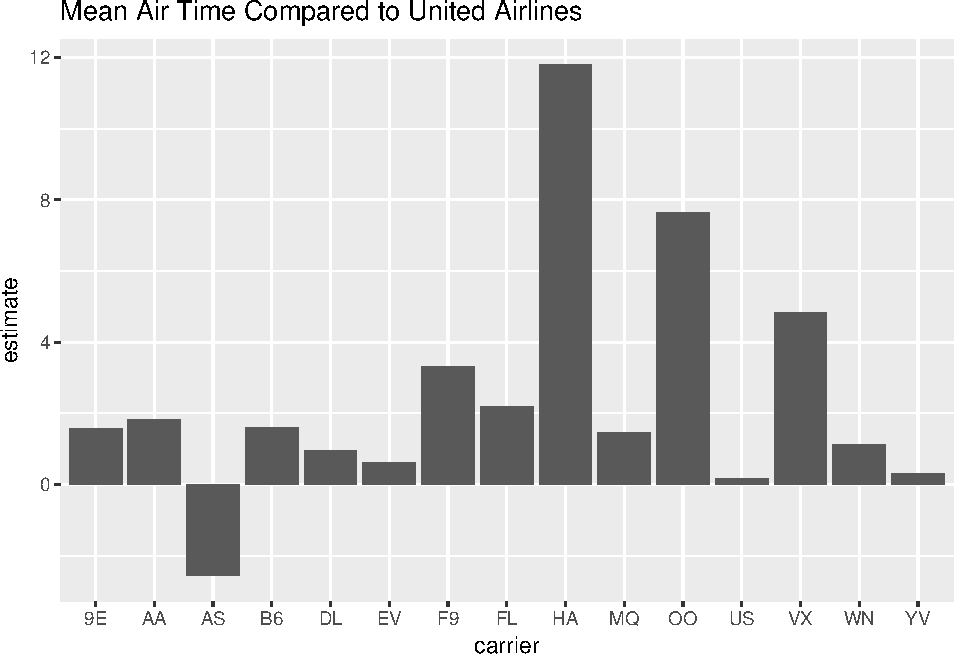
\includegraphics{01-Introduction_files/figure-latex/unnamed-chunk-36-1.pdf}

The results are similar to the previous linear mode except that this
time SkyWest Airlines shows much longer air time.

Before wrapping up, our final model is a check for the robustness of the
above results. We would like to replace the date and hour fixed effects
in the previous model with date-hour fixed effects (i.e., the
interaction between date and hour). We could add such fixed effects
using \texttt{time\_hour} variable defined above. However, that would
mean adding nearly 7,000 dummy variables to our linear regression, which
is computationally too intensive.

To work around this issue, we approximate this estimation by
pre-processing the dependent variable. Specifically, we calculate the
average air time for each combination of \texttt{time\_hour} and
\texttt{dest} and define a new dependent variable by subtracting this
average value from the original air time variable (i.e., the new
variable is centered at zero-mean for each combination of
\texttt{time\_hour} and \texttt{dest}). Then, we estimate a linear model
with carrier and destination fixed effects.

\begin{Shaded}
\begin{Highlighting}[]
\NormalTok{## Adding time_hour fixed effects is too computationally intensive }
\CommentTok{# f1 <- flights %>%}
\CommentTok{#  with(}
\CommentTok{#    lm( air_time  ~  as.factor(carrier) + as.factor(dest) + as.factor(time_hour))   }
\CommentTok{#  )}

\KeywordTok{unique}\NormalTok{(flights2$time_hour) %>%}\StringTok{ }\KeywordTok{length}\NormalTok{()  }\CommentTok{# 6,936 unique time_hour }
\end{Highlighting}
\end{Shaded}

\begin{verbatim}
## [1] 6936
\end{verbatim}

\begin{Shaded}
\begin{Highlighting}[]
\NormalTok{flights2 <-}\StringTok{ }\NormalTok{flights2 %>%}\StringTok{ }
\StringTok{  }\KeywordTok{group_by}\NormalTok{(dest, time_hour) %>%}\StringTok{   }
\StringTok{  }\KeywordTok{mutate}\NormalTok{(}
    \DataTypeTok{air_time_centered =} \NormalTok{air_time -}\StringTok{ }\KeywordTok{mean}\NormalTok{(air_time, }\DataTypeTok{na.rm=}\OtherTok{TRUE}\NormalTok{) }
  \NormalTok{)}

\NormalTok{f3 <-}\StringTok{ }\NormalTok{flights2 %>%}
\StringTok{ }\KeywordTok{with}\NormalTok{(}
   \KeywordTok{lm}\NormalTok{( air_time_centered  ~}\StringTok{  }\KeywordTok{as.factor}\NormalTok{(carrier) +}\StringTok{ }\KeywordTok{as.factor}\NormalTok{(dest) )}
 \NormalTok{)}
  
\NormalTok{lm_rlt3 <-}\StringTok{ }\KeywordTok{clean_lm_rlt}\NormalTok{(f3)}
\NormalTok{lm_rlt3 %>%}\StringTok{ }\KeywordTok{kable}\NormalTok{(}\DataTypeTok{digit=}\DecValTok{2}\NormalTok{) }\CommentTok{# Note: standard errors, t-stat, and p-val are incorrect}
\end{Highlighting}
\end{Shaded}

\begin{tabular}{l|l|r|r|r|r|r}
\hline
carrier & name & n\_obs & estimate & std.error & statistic & p.value\\
\hline
UA & United Air Lines Inc. & 58665 & NA & NA & NA & NA\\
\hline
B6 & JetBlue Airways & 54635 & 0.82 & 0.03 & 32.24 & 0.00\\
\hline
EV & ExpressJet Airlines Inc. & 54173 & 0.88 & 0.03 & 26.50 & 0.00\\
\hline
DL & Delta Air Lines Inc. & 48110 & 0.52 & 0.03 & 19.85 & 0.00\\
\hline
AA & American Airlines Inc. & 32729 & 1.20 & 0.03 & 41.06 & 0.00\\
\hline
MQ & Envoy Air & 26397 & 1.00 & 0.04 & 27.84 & 0.00\\
\hline
US & US Airways Inc. & 20536 & -0.09 & 0.04 & -2.21 & 0.03\\
\hline
9E & Endeavor Air Inc. & 18460 & 1.27 & 0.04 & 33.07 & 0.00\\
\hline
WN & Southwest Airlines Co. & 12275 & 1.30 & 0.05 & 24.70 & 0.00\\
\hline
VX & Virgin America & 5162 & 3.47 & 0.06 & 62.59 & 0.00\\
\hline
FL & AirTran Airways Corporation & 3260 & 1.78 & 0.08 & 21.48 & 0.00\\
\hline
AS & Alaska Airlines Inc. & 714 & -2.86 & 0.15 & -19.15 & 0.00\\
\hline
F9 & Frontier Airlines Inc. & 685 & 1.99 & 0.14 & 13.73 & 0.00\\
\hline
YV & Mesa Airlines Inc. & 601 & 0.78 & 0.16 & 4.89 & 0.00\\
\hline
HA & Hawaiian Airlines Inc. & 342 & 1.34 & 0.27 & 4.96 & 0.00\\
\hline
OO & SkyWest Airlines Inc. & 32 & 3.50 & 0.67 & 5.26 & 0.00\\
\hline
\end{tabular}

\begin{Shaded}
\begin{Highlighting}[]
\NormalTok{lm_rlt3 %>%}\StringTok{ }\KeywordTok{filter}\NormalTok{(carrier!=}\StringTok{'UA'}\NormalTok{) %>%}
\StringTok{  }\KeywordTok{ggplot}\NormalTok{(}\KeywordTok{aes}\NormalTok{(}\DataTypeTok{x =} \NormalTok{carrier, }\DataTypeTok{y =} \NormalTok{estimate)) +}\StringTok{ }\KeywordTok{geom_col}\NormalTok{() +}
\StringTok{  }\KeywordTok{labs}\NormalTok{(}\DataTypeTok{title =} \StringTok{"Mean Air Time Compared to United Airlines: Robustness Check"}\NormalTok{)}
\end{Highlighting}
\end{Shaded}

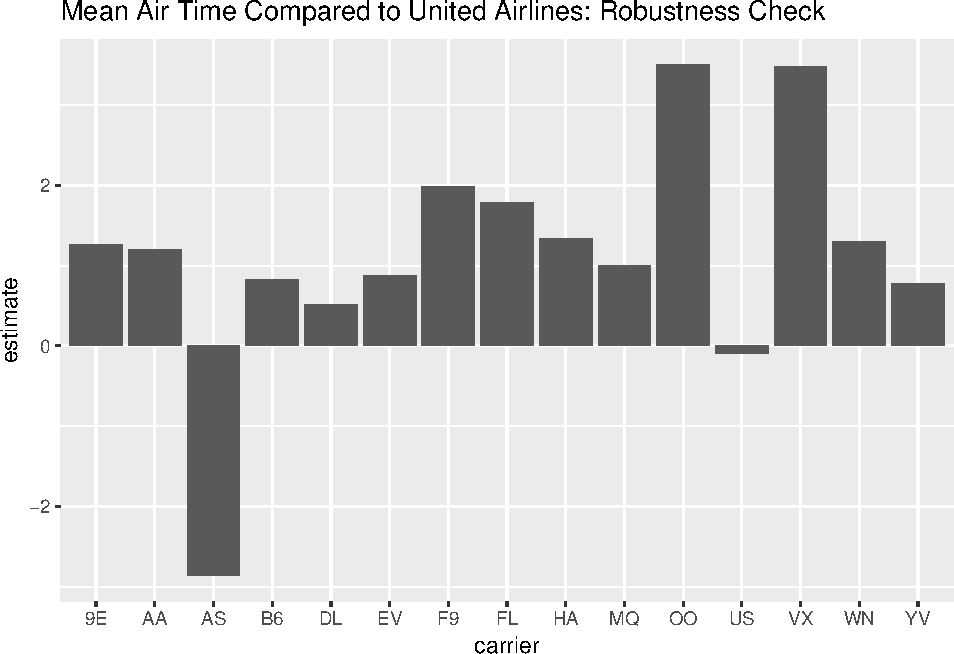
\includegraphics{01-Introduction_files/figure-latex/unnamed-chunk-37-1.pdf}

The point estimates should be \emph{approximately} close to what we
would obtain if we regress \texttt{air\_time} on the fixed effects of
\texttt{carrier}, \texttt{dest}, and \texttt{time\_hour}. However, the
standard errors are not correctly displayed in the table because the
centered variable has less total variation compared to the original
\texttt{air\_time} variable. (Correct standard errors can be obtained,
for example, through a bootstrapping technique.)

Overall, we see again a tendency that low-cost carriers like Sky West
Airlines, Virgin America, Frontier Airlines, and Air Tran show
particularly longer air time than United Airlines. Jet Blue Airways,
another low-cost carrier, shows a less obvious difference from United
Airlines, possibly suggesting that their operation focused on the East
Cost is efficient for the flights departing from New York City. Hawaiian
Airlines and Alaskan Airlines appear to be somewhat different from other
carriers perhaps because they are more specialized in particular flight
times and destinations compared to their rivals. In particular, the
flights to Hawaii may have distinct delay patterns that are concentrated
on certain date-hours of the peak vacation seasons.

\section{Reflections}\label{reflections}

In this introduction, we have reviewed the tools of \texttt{deplyr} and
\texttt{ggplot2} packages as a starting point for data analyses and
visualization in R. This new generation of tools is a data exploration
language as much as a set of functions to shortcut traditional data
manipulation methods in R. This language provides a very intuitive
system of translating our inquiries to the data analysis in R.

Using the flight dataset, we have also investigated flight delay
patterns. We find that airport congestion is unlikely a major cause of
delay in New York City. There are small differences in the air time
(e.g.~less than 5 minutes) across carriers for a given destination
although it remains unclear how this relates to the delay patterns.

In fact, the concept of ``delay'' is complicated because it is defined
in reference to the scheduled departure and arrival times, which may
differ by carrier. A delay would not include the time sitting in the
airplane before taking off or after landing as long as it is within the
schedule. It might be more interesting to compare scheduled flight
duration instead of delays or air time. (Such an analysis would involve
somewhat complicated manipulations of date and time with our flight
data.)

This leads us to the final point of this exercise; an interesting data
analysis requires \textbf{knowledge on the real-world process that
generated the data} and \textbf{the ability to ask interesting
questions}. \texttt{deplyr} and \texttt{ggplot2} packages can let you
employ a variety of data analytics tools with ease, but the ultimate
power of the analysis will always rest on your knowledge and creativity.

\chapter{Essentials}\label{essentials}

2017-04-08: {\emph{VERY Preliminary!}}

This section provides an overview of the essential concepts for
manipulating data and programming in R.

\section{Cheatsheets}\label{cheatsheets}

Cheatsheets are useful for glancing at various functions.

\begin{itemize}
\item
  \href{http://github.com/rstudio/cheatsheets/raw/master/source/pdfs/base-r.pdf}{Base
  R}
\item
  \href{https://www.rstudio.com/wp-content/uploads/2016/01/rstudio-IDE-cheatsheet.pdf}{RStudio
  IDE}
\item
  \href{https://github.com/rstudio/cheatsheets/raw/master/source/pdfs/data-transformation-cheatsheet.pdf}{dplyr}
\item
  \href{https://www.rstudio.com/wp-content/uploads/2016/11/ggplot2-cheatsheet-2.1.pdf}{ggplot2}
\end{itemize}

\section{Data types}\label{data-types}

\subsection{Atomic}\label{atomic}

In most cases, each atomic element has a type (mode) of;

\begin{itemize}
\item
  \texttt{numeric}: number
\item
  \texttt{logical}: TRUE or FALSE (T or F for shortcuts)
\item
  \texttt{character}: character string
\item
  \texttt{factor}: a level of categorical variable
\end{itemize}

Other types include
\href{http://www.statmethods.net/input/dates.html}{date} and nonexistent
\texttt{NULL}. The factor is also a \emph{class} of its own, meaning
that many R functions apply operations that are specific to the
\emph{factor class}.

\begin{Shaded}
\begin{Highlighting}[]
\CommentTok{# assess objects 123, "abc", and TRUE for their types }
\KeywordTok{str}\NormalTok{(}\DecValTok{123}\NormalTok{)  }\CommentTok{# str() returns the structure}
\end{Highlighting}
\end{Shaded}

\begin{verbatim}
##  num 123
\end{verbatim}

\begin{Shaded}
\begin{Highlighting}[]
\KeywordTok{str}\NormalTok{(}\StringTok{"abc"}\NormalTok{)}
\end{Highlighting}
\end{Shaded}

\begin{verbatim}
##  chr "abc"
\end{verbatim}

\begin{Shaded}
\begin{Highlighting}[]
\KeywordTok{str}\NormalTok{(}\OtherTok{TRUE}\NormalTok{)}
\end{Highlighting}
\end{Shaded}

\begin{verbatim}
##  logi TRUE
\end{verbatim}

\begin{Shaded}
\begin{Highlighting}[]
\KeywordTok{c}\NormalTok{(}\KeywordTok{is.numeric}\NormalTok{(}\DecValTok{123}\NormalTok{), }\KeywordTok{is.numeric}\NormalTok{(}\StringTok{"abc"}\NormalTok{), }\KeywordTok{is.numeric}\NormalTok{(}\OtherTok{TRUE}\NormalTok{))}
\end{Highlighting}
\end{Shaded}

\begin{verbatim}
## [1]  TRUE FALSE FALSE
\end{verbatim}

\begin{Shaded}
\begin{Highlighting}[]
\KeywordTok{c}\NormalTok{(}\KeywordTok{is.logical}\NormalTok{(}\DecValTok{123}\NormalTok{), }\KeywordTok{is.logical}\NormalTok{(}\StringTok{"abc"}\NormalTok{), }\KeywordTok{is.logical}\NormalTok{(}\OtherTok{TRUE}\NormalTok{))}
\end{Highlighting}
\end{Shaded}

\begin{verbatim}
## [1] FALSE FALSE  TRUE
\end{verbatim}

\begin{Shaded}
\begin{Highlighting}[]
\KeywordTok{c}\NormalTok{(}\KeywordTok{is.character}\NormalTok{(}\DecValTok{123}\NormalTok{), }\KeywordTok{is.character}\NormalTok{(}\StringTok{"abc"}\NormalTok{), }\KeywordTok{is.character}\NormalTok{(}\OtherTok{TRUE}\NormalTok{))}
\end{Highlighting}
\end{Shaded}

\begin{verbatim}
## [1] FALSE  TRUE FALSE
\end{verbatim}

\begin{Shaded}
\begin{Highlighting}[]
\CommentTok{# "<-" means an assignment from right to left}
\NormalTok{factor1 <-}\StringTok{ }\KeywordTok{as.factor}\NormalTok{(}\KeywordTok{c}\NormalTok{(}\DecValTok{1}\NormalTok{,}\DecValTok{2}\NormalTok{,}\DecValTok{3}\NormalTok{)) }\CommentTok{# Looks like numeric but not}
\NormalTok{factor1}
\end{Highlighting}
\end{Shaded}

\begin{verbatim}
## [1] 1 2 3
## Levels: 1 2 3
\end{verbatim}

\begin{Shaded}
\begin{Highlighting}[]
\NormalTok{factor2 <-}\StringTok{ }\KeywordTok{as.factor}\NormalTok{(}\KeywordTok{c}\NormalTok{(}\StringTok{"a"}\NormalTok{,}\StringTok{"b"}\NormalTok{,}\StringTok{"c"}\NormalTok{))  }\CommentTok{# Looks like characters but not}
\NormalTok{factor2}
\end{Highlighting}
\end{Shaded}

\begin{verbatim}
## [1] a b c
## Levels: a b c
\end{verbatim}

\begin{Shaded}
\begin{Highlighting}[]
\NormalTok{factor3 <-}\StringTok{ }\KeywordTok{as.factor}\NormalTok{(}\KeywordTok{c}\NormalTok{(}\OtherTok{TRUE}\NormalTok{,}\OtherTok{FALSE}\NormalTok{,T)) }\CommentTok{# Looks like logicals but not}
\NormalTok{factor3}
\end{Highlighting}
\end{Shaded}

\begin{verbatim}
## [1] TRUE  FALSE TRUE 
## Levels: FALSE TRUE
\end{verbatim}

\begin{Shaded}
\begin{Highlighting}[]
\KeywordTok{c}\NormalTok{(}\KeywordTok{is.factor}\NormalTok{(factor1[}\DecValTok{1}\NormalTok{]), }\KeywordTok{is.factor}\NormalTok{(factor2[}\DecValTok{1}\NormalTok{]), }\KeywordTok{is.factor}\NormalTok{(factor3[}\DecValTok{1}\NormalTok{]))}
\end{Highlighting}
\end{Shaded}

\begin{verbatim}
## [1] TRUE TRUE TRUE
\end{verbatim}

\begin{Shaded}
\begin{Highlighting}[]
\CommentTok{# Extract the first element (factor1[1] etc.) }
\NormalTok{factor1[}\DecValTok{1}\NormalTok{]}
\end{Highlighting}
\end{Shaded}

\begin{verbatim}
## [1] 1
## Levels: 1 2 3
\end{verbatim}

\begin{Shaded}
\begin{Highlighting}[]
\NormalTok{factor2[}\DecValTok{2}\NormalTok{]}
\end{Highlighting}
\end{Shaded}

\begin{verbatim}
## [1] b
## Levels: a b c
\end{verbatim}

\begin{Shaded}
\begin{Highlighting}[]
\NormalTok{factor3[}\DecValTok{3}\NormalTok{]}
\end{Highlighting}
\end{Shaded}

\begin{verbatim}
## [1] TRUE
## Levels: FALSE TRUE
\end{verbatim}

\texttt{NULL} has zero-length. Also, empty numeric, logical, and
character objects have zero-length.

\begin{Shaded}
\begin{Highlighting}[]
\KeywordTok{length}\NormalTok{(}\OtherTok{NULL}\NormalTok{) }
\end{Highlighting}
\end{Shaded}

\begin{verbatim}
## [1] 0
\end{verbatim}

\begin{Shaded}
\begin{Highlighting}[]
\KeywordTok{length}\NormalTok{(}\KeywordTok{numeric}\NormalTok{(}\DecValTok{0}\NormalTok{))  }\CommentTok{# numeric(N) returns a vector of N zeros }
\end{Highlighting}
\end{Shaded}

\begin{verbatim}
## [1] 0
\end{verbatim}

\begin{Shaded}
\begin{Highlighting}[]
\KeywordTok{length}\NormalTok{(}\KeywordTok{logical}\NormalTok{(}\DecValTok{0}\NormalTok{))  }\CommentTok{# logical(N) returns a vector of N FALSE objects}
\end{Highlighting}
\end{Shaded}

\begin{verbatim}
## [1] 0
\end{verbatim}

\begin{Shaded}
\begin{Highlighting}[]
\KeywordTok{length}\NormalTok{(}\KeywordTok{character}\NormalTok{(}\DecValTok{0}\NormalTok{)) }\CommentTok{# character(N) returns a vector of N "" objects}
\end{Highlighting}
\end{Shaded}

\begin{verbatim}
## [1] 0
\end{verbatim}

Each \textbf{vector} has a type of \texttt{numeric}, \texttt{logical},
\texttt{character}, or \texttt{factor}. Each \textbf{matrix} has a type
of \texttt{numeric}, \texttt{logical}, or \texttt{character}. A
\textbf{data frame} can contain mixed types across columns where each
column (e.g., a variable) has a type of \texttt{numeric},
\texttt{logical}, \texttt{character} or \texttt{factor}.

\begin{Shaded}
\begin{Highlighting}[]
\NormalTok{vector1 <-}\StringTok{ }\KeywordTok{c}\NormalTok{(}\DecValTok{1}\NormalTok{, }\OtherTok{NA}\NormalTok{, }\DecValTok{2}\NormalTok{, }\DecValTok{3}\NormalTok{) }\CommentTok{# read as numeric}
\NormalTok{vector1}
\end{Highlighting}
\end{Shaded}

\begin{verbatim}
## [1]  1 NA  2  3
\end{verbatim}

\begin{Shaded}
\begin{Highlighting}[]
\NormalTok{vector2 <-}\StringTok{ }\KeywordTok{c}\NormalTok{(}\OtherTok{TRUE}\NormalTok{, }\OtherTok{FALSE}\NormalTok{, T, F) }\CommentTok{# read as logical}
\NormalTok{vector2}
\end{Highlighting}
\end{Shaded}

\begin{verbatim}
## [1]  TRUE FALSE  TRUE FALSE
\end{verbatim}

\begin{Shaded}
\begin{Highlighting}[]
\NormalTok{vector3 <-}\StringTok{ }\KeywordTok{c}\NormalTok{(}\DecValTok{1}\NormalTok{, }\OtherTok{NA}\NormalTok{, }\StringTok{"abc"}\NormalTok{, }\OtherTok{TRUE}\NormalTok{, }\StringTok{"TRUE"}\NormalTok{) }\CommentTok{# read as character}
\NormalTok{vector3}
\end{Highlighting}
\end{Shaded}

\begin{verbatim}
## [1] "1"    NA     "abc"  "TRUE" "TRUE"
\end{verbatim}

\begin{Shaded}
\begin{Highlighting}[]
\NormalTok{vector4 <-}\StringTok{ }\KeywordTok{as.factor}\NormalTok{(}\KeywordTok{c}\NormalTok{(}\DecValTok{1}\NormalTok{, }\OtherTok{NA}\NormalTok{, }\StringTok{"abc"}\NormalTok{, }\OtherTok{TRUE}\NormalTok{, }\StringTok{"TRUE"}\NormalTok{)) }\CommentTok{# read as factor }
\NormalTok{vector4}
\end{Highlighting}
\end{Shaded}

\begin{verbatim}
## [1] 1    <NA> abc  TRUE TRUE
## Levels: 1 abc TRUE
\end{verbatim}

\begin{Shaded}
\begin{Highlighting}[]
\NormalTok{matrix1 <-}\StringTok{ }\KeywordTok{matrix}\NormalTok{(}\KeywordTok{c}\NormalTok{(}\DecValTok{1}\NormalTok{:}\DecValTok{6}\NormalTok{), }\DataTypeTok{nrow =} \DecValTok{3}\NormalTok{) }\CommentTok{# read as numeric}
\NormalTok{matrix1}
\end{Highlighting}
\end{Shaded}

\begin{verbatim}
##      [,1] [,2]
## [1,]    1    4
## [2,]    2    5
## [3,]    3    6
\end{verbatim}

\begin{Shaded}
\begin{Highlighting}[]
\NormalTok{matrix2 <-}\StringTok{ }\KeywordTok{matrix}\NormalTok{(}\KeywordTok{c}\NormalTok{(}\OtherTok{TRUE}\NormalTok{,}\OtherTok{FALSE}\NormalTok{,}\KeywordTok{rep}\NormalTok{(T,}\DecValTok{3}\NormalTok{),F), }\DataTypeTok{nrow =} \DecValTok{3}\NormalTok{)  }\CommentTok{# read as logical}
\NormalTok{matrix2}
\end{Highlighting}
\end{Shaded}

\begin{verbatim}
##       [,1]  [,2]
## [1,]  TRUE  TRUE
## [2,] FALSE  TRUE
## [3,]  TRUE FALSE
\end{verbatim}

\begin{Shaded}
\begin{Highlighting}[]
\NormalTok{matrix3 <-}\StringTok{ }\KeywordTok{matrix}\NormalTok{(}\KeywordTok{c}\NormalTok{(}\DecValTok{1}\NormalTok{,}\DecValTok{2}\NormalTok{,}\DecValTok{3}\NormalTok{,}\StringTok{"a"}\NormalTok{,}\StringTok{"b"}\NormalTok{,}\StringTok{"abc"}\NormalTok{), }\DataTypeTok{nrow =} \DecValTok{3}\NormalTok{) }\CommentTok{# read as character}
\NormalTok{matrix3}
\end{Highlighting}
\end{Shaded}

\begin{verbatim}
##      [,1] [,2] 
## [1,] "1"  "a"  
## [2,] "2"  "b"  
## [3,] "3"  "abc"
\end{verbatim}

\begin{Shaded}
\begin{Highlighting}[]
\NormalTok{df1 <-}\StringTok{ }\KeywordTok{data.frame}\NormalTok{(}
        \DataTypeTok{num  =} \KeywordTok{c}\NormalTok{(}\DecValTok{1}\NormalTok{,}\DecValTok{2}\NormalTok{,}\DecValTok{3}\NormalTok{),           }\CommentTok{# read as numeric}
        \DataTypeTok{fac1 =} \KeywordTok{c}\NormalTok{(}\StringTok{"a"}\NormalTok{,}\StringTok{"b"}\NormalTok{,}\StringTok{"abc"}\NormalTok{),   }\CommentTok{# read as factor}
        \DataTypeTok{logi =} \KeywordTok{c}\NormalTok{(}\OtherTok{TRUE}\NormalTok{, }\OtherTok{FALSE}\NormalTok{, T),  }\CommentTok{# read as logical}
        \DataTypeTok{fac2  =} \KeywordTok{c}\NormalTok{(}\DecValTok{1}\NormalTok{,}\StringTok{"a"}\NormalTok{,}\OtherTok{TRUE}\NormalTok{)      }\CommentTok{# read as factor}
       \NormalTok{)  }
\NormalTok{df1}
\end{Highlighting}
\end{Shaded}

\begin{verbatim}
##   num fac1  logi fac2
## 1   1    a  TRUE    1
## 2   2    b FALSE    a
## 3   3  abc  TRUE TRUE
\end{verbatim}

\begin{Shaded}
\begin{Highlighting}[]
\NormalTok{df1$num   }\CommentTok{# "$" symbol is used to extract a column }
\end{Highlighting}
\end{Shaded}

\begin{verbatim}
## [1] 1 2 3
\end{verbatim}

\begin{Shaded}
\begin{Highlighting}[]
\NormalTok{df1$fac1  }\CommentTok{# character type is converted into a factor }
\end{Highlighting}
\end{Shaded}

\begin{verbatim}
## [1] a   b   abc
## Levels: a abc b
\end{verbatim}

\begin{Shaded}
\begin{Highlighting}[]
\NormalTok{df1$logi}
\end{Highlighting}
\end{Shaded}

\begin{verbatim}
## [1]  TRUE FALSE  TRUE
\end{verbatim}

\begin{Shaded}
\begin{Highlighting}[]
\NormalTok{df1$fac2  }\CommentTok{# mixed types within a column is converted into a factor}
\end{Highlighting}
\end{Shaded}

\begin{verbatim}
## [1] 1    a    TRUE
## Levels: 1 a TRUE
\end{verbatim}

\begin{Shaded}
\begin{Highlighting}[]
\CommentTok{# additional argument "stringsAsFactors = FALSE" preserves character types.}
\NormalTok{df2 <-}\StringTok{ }\KeywordTok{data.frame}\NormalTok{(}
        \DataTypeTok{num  =} \KeywordTok{c}\NormalTok{(}\DecValTok{1}\NormalTok{,}\DecValTok{2}\NormalTok{,}\DecValTok{3}\NormalTok{),           }\CommentTok{# read as numeric}
        \DataTypeTok{char =} \KeywordTok{c}\NormalTok{(}\StringTok{"a"}\NormalTok{,}\StringTok{"b"}\NormalTok{,}\StringTok{"abc"}\NormalTok{),   }\CommentTok{# read as character}
        \DataTypeTok{logi =} \KeywordTok{c}\NormalTok{(}\OtherTok{TRUE}\NormalTok{, }\OtherTok{FALSE}\NormalTok{, T),  }\CommentTok{# read as logical}
        \DataTypeTok{fac2  =} \KeywordTok{as.factor}\NormalTok{(}\KeywordTok{c}\NormalTok{(}\DecValTok{1}\NormalTok{,}\StringTok{"a"}\NormalTok{,}\OtherTok{TRUE}\NormalTok{)),      }\CommentTok{# read as factor}
        \DataTypeTok{stringsAsFactors =} \OtherTok{FALSE}
       \NormalTok{)  }
\NormalTok{df2}
\end{Highlighting}
\end{Shaded}

\begin{verbatim}
##   num char  logi fac2
## 1   1    a  TRUE    1
## 2   2    b FALSE    a
## 3   3  abc  TRUE TRUE
\end{verbatim}

\begin{Shaded}
\begin{Highlighting}[]
\NormalTok{df2$num  }
\end{Highlighting}
\end{Shaded}

\begin{verbatim}
## [1] 1 2 3
\end{verbatim}

\begin{Shaded}
\begin{Highlighting}[]
\NormalTok{df2$char}
\end{Highlighting}
\end{Shaded}

\begin{verbatim}
## [1] "a"   "b"   "abc"
\end{verbatim}

\begin{Shaded}
\begin{Highlighting}[]
\NormalTok{df2$logi}
\end{Highlighting}
\end{Shaded}

\begin{verbatim}
## [1]  TRUE FALSE  TRUE
\end{verbatim}

\begin{Shaded}
\begin{Highlighting}[]
\NormalTok{df2$fac2}
\end{Highlighting}
\end{Shaded}

\begin{verbatim}
## [1] 1    a    TRUE
## Levels: 1 a TRUE
\end{verbatim}

\subsection{Factor}\label{factor}

A factor object is defined with a set of categorical levels, which may
be labeled. The levels are either \textbf{ordered} (defined by
\texttt{ordered()}) or \textbf{unordered} (defined by
\texttt{factor()}). Ordered factor objects are treated in the specific
order by certain statistical and graphical procedures.

\begin{Shaded}
\begin{Highlighting}[]
\CommentTok{# We will convert the columns of df into factors   }
\NormalTok{df <-}\StringTok{ }\KeywordTok{data.frame}\NormalTok{(}
      \DataTypeTok{fac1 =} \KeywordTok{c}\NormalTok{(}\DecValTok{0}\NormalTok{,}\DecValTok{1}\NormalTok{,}\DecValTok{1}\NormalTok{,}\DecValTok{4}\NormalTok{,}\DecValTok{4}\NormalTok{,}\DecValTok{2}\NormalTok{,}\DecValTok{2}\NormalTok{,}\DecValTok{3}\NormalTok{),}
      \DataTypeTok{fac2 =} \KeywordTok{c}\NormalTok{(}\DecValTok{1}\NormalTok{,}\DecValTok{2}\NormalTok{,}\DecValTok{3}\NormalTok{,}\DecValTok{1}\NormalTok{,}\DecValTok{1}\NormalTok{,}\DecValTok{2}\NormalTok{,}\DecValTok{2}\NormalTok{,}\DecValTok{3}\NormalTok{),}
      \DataTypeTok{fac3 =} \KeywordTok{c}\NormalTok{(}\DecValTok{4}\NormalTok{,}\DecValTok{2}\NormalTok{,}\DecValTok{3}\NormalTok{,}\DecValTok{4}\NormalTok{,}\DecValTok{4}\NormalTok{,}\DecValTok{2}\NormalTok{,}\DecValTok{2}\NormalTok{,}\DecValTok{3}\NormalTok{)}
      \NormalTok{)}

\CommentTok{# convert fac1 to ordered factors}
\NormalTok{df$fac1 <-}\StringTok{ }\KeywordTok{ordered}\NormalTok{(df$fac1,}
                  \DataTypeTok{levels =} \KeywordTok{c}\NormalTok{(}\DecValTok{0}\NormalTok{,}\DecValTok{4}\NormalTok{,}\DecValTok{3}\NormalTok{,}\DecValTok{2}\NormalTok{,}\DecValTok{1}\NormalTok{) }\CommentTok{# defines the order}
                  \NormalTok{) }
\NormalTok{df$fac1}
\end{Highlighting}
\end{Shaded}

\begin{verbatim}
## [1] 0 1 1 4 4 2 2 3
## Levels: 0 < 4 < 3 < 2 < 1
\end{verbatim}

\begin{Shaded}
\begin{Highlighting}[]
\KeywordTok{summary}\NormalTok{(df$fac1)  }\CommentTok{# gives the table of counts for each level}
\end{Highlighting}
\end{Shaded}

\begin{verbatim}
## 0 4 3 2 1 
## 1 2 1 2 2
\end{verbatim}

\begin{Shaded}
\begin{Highlighting}[]
\CommentTok{# convert fac2 to unordered factors with labels}
\NormalTok{df$fac2 <-}\StringTok{ }\KeywordTok{factor}\NormalTok{(df$fac2,}
                  \DataTypeTok{levels =} \KeywordTok{c}\NormalTok{(}\DecValTok{1}\NormalTok{,}\DecValTok{2}\NormalTok{,}\DecValTok{3}\NormalTok{), }\CommentTok{#  no particular order}
                  \CommentTok{# attach labels to factors: 1=red, 2=blue, 3=green}
                  \DataTypeTok{labels =} \KeywordTok{c}\NormalTok{(}\StringTok{"red"}\NormalTok{, }\StringTok{"blue"}\NormalTok{, }\StringTok{"green"}\NormalTok{)}
                  \NormalTok{) }
\NormalTok{df$fac2}
\end{Highlighting}
\end{Shaded}

\begin{verbatim}
## [1] red   blue  green red   red   blue  blue  green
## Levels: red blue green
\end{verbatim}

\begin{Shaded}
\begin{Highlighting}[]
\KeywordTok{summary}\NormalTok{(df$fac2)                }
\end{Highlighting}
\end{Shaded}

\begin{verbatim}
##   red  blue green 
##     3     3     2
\end{verbatim}

\begin{Shaded}
\begin{Highlighting}[]
\CommentTok{# convert fac3 to ordered factors with labels}
\NormalTok{df$fac3 <-}\StringTok{ }\KeywordTok{ordered}\NormalTok{(df$fac3,}
                  \DataTypeTok{levels =} \KeywordTok{c}\NormalTok{(}\DecValTok{2}\NormalTok{,}\DecValTok{3}\NormalTok{,}\DecValTok{4}\NormalTok{),}
                  \CommentTok{# attach labels to factors: 2=Low, 3=Medium, 4=High}
                  \DataTypeTok{labels =} \KeywordTok{c}\NormalTok{(}\StringTok{"Low"}\NormalTok{, }\StringTok{"Medium"}\NormalTok{, }\StringTok{"High"}\NormalTok{)}
                  \NormalTok{) }
\NormalTok{df$fac3}
\end{Highlighting}
\end{Shaded}

\begin{verbatim}
## [1] High   Low    Medium High   High   Low    Low    Medium
## Levels: Low < Medium < High
\end{verbatim}

\begin{Shaded}
\begin{Highlighting}[]
\KeywordTok{summary}\NormalTok{(df$fac3)}
\end{Highlighting}
\end{Shaded}

\begin{verbatim}
##    Low Medium   High 
##      3      2      3
\end{verbatim}

\subsection{Matrix}\label{matrix}

\texttt{matrix()} defines a matrix from a vector. The default is to
arrange the vector by column (\texttt{byrow\ =\ FALSE}).

\begin{Shaded}
\begin{Highlighting}[]
\CommentTok{# byrow = FALSE  (the default)}
\KeywordTok{matrix}\NormalTok{(}\DataTypeTok{data =} \KeywordTok{c}\NormalTok{(}\DecValTok{1}\NormalTok{:}\DecValTok{6}\NormalTok{), }\DataTypeTok{nrow =} \DecValTok{2}\NormalTok{, }\DataTypeTok{ncol =} \DecValTok{3}\NormalTok{, }\DataTypeTok{byrow =} \OtherTok{FALSE}\NormalTok{, }\DataTypeTok{dimnames =} \OtherTok{NULL}\NormalTok{)}
\end{Highlighting}
\end{Shaded}

\begin{verbatim}
##      [,1] [,2] [,3]
## [1,]    1    3    5
## [2,]    2    4    6
\end{verbatim}

\begin{Shaded}
\begin{Highlighting}[]
\CommentTok{# byrow = TRUE }
\KeywordTok{matrix}\NormalTok{(}\DataTypeTok{data =} \KeywordTok{c}\NormalTok{(}\DecValTok{1}\NormalTok{:}\DecValTok{6}\NormalTok{), }\DataTypeTok{nrow =} \DecValTok{2}\NormalTok{, }\DataTypeTok{ncol =} \DecValTok{3}\NormalTok{, }\DataTypeTok{byrow =} \OtherTok{TRUE}\NormalTok{, }\DataTypeTok{dimnames =} \OtherTok{NULL}\NormalTok{)}
\end{Highlighting}
\end{Shaded}

\begin{verbatim}
##      [,1] [,2] [,3]
## [1,]    1    2    3
## [2,]    4    5    6
\end{verbatim}

\begin{Shaded}
\begin{Highlighting}[]
\CommentTok{# give row and column names to a matrix }
\NormalTok{mat1 <-}\StringTok{ }\KeywordTok{matrix}\NormalTok{(}\DataTypeTok{data =} \KeywordTok{c}\NormalTok{(}\DecValTok{1}\NormalTok{:}\DecValTok{6}\NormalTok{), }\DataTypeTok{nrow =} \DecValTok{2}\NormalTok{, }\DataTypeTok{ncol =} \DecValTok{3}\NormalTok{, }\DataTypeTok{byrow =} \OtherTok{FALSE}\NormalTok{, }
       \DataTypeTok{dimnames =} \KeywordTok{list}\NormalTok{(}\KeywordTok{c}\NormalTok{(}\StringTok{"r1"}\NormalTok{,}\StringTok{"r2"}\NormalTok{), }\KeywordTok{c}\NormalTok{(}\StringTok{"c1"}\NormalTok{,}\StringTok{"c2"}\NormalTok{,}\StringTok{"c3"}\NormalTok{)))}
\NormalTok{mat1}
\end{Highlighting}
\end{Shaded}

\begin{verbatim}
##    c1 c2 c3
## r1  1  3  5
## r2  2  4  6
\end{verbatim}

\begin{Shaded}
\begin{Highlighting}[]
\KeywordTok{dim}\NormalTok{(mat1)  }\CommentTok{# dimension: row by column}
\end{Highlighting}
\end{Shaded}

\begin{verbatim}
## [1] 2 3
\end{verbatim}

\begin{Shaded}
\begin{Highlighting}[]
\KeywordTok{colnames}\NormalTok{(mat1)}
\end{Highlighting}
\end{Shaded}

\begin{verbatim}
## [1] "c1" "c2" "c3"
\end{verbatim}

\begin{Shaded}
\begin{Highlighting}[]
\KeywordTok{rownames}\NormalTok{(mat1)}
\end{Highlighting}
\end{Shaded}

\begin{verbatim}
## [1] "r1" "r2"
\end{verbatim}

\begin{Shaded}
\begin{Highlighting}[]
\KeywordTok{colnames}\NormalTok{(mat1) <-}\StringTok{ }\KeywordTok{c}\NormalTok{(}\StringTok{"v1"}\NormalTok{,}\StringTok{"v2"}\NormalTok{,}\StringTok{"v3"}\NormalTok{)  }\CommentTok{# change column names by assignment "<-" }
\NormalTok{mat1}
\end{Highlighting}
\end{Shaded}

\begin{verbatim}
##    v1 v2 v3
## r1  1  3  5
## r2  2  4  6
\end{verbatim}

\begin{Shaded}
\begin{Highlighting}[]
\CommentTok{# R makes a guess when only nrow or ncol is supplied}
\KeywordTok{matrix}\NormalTok{(}\DataTypeTok{data =} \KeywordTok{c}\NormalTok{(}\DecValTok{1}\NormalTok{:}\DecValTok{6}\NormalTok{), }\DataTypeTok{nrow =} \DecValTok{2}\NormalTok{)}
\end{Highlighting}
\end{Shaded}

\begin{verbatim}
##      [,1] [,2] [,3]
## [1,]    1    3    5
## [2,]    2    4    6
\end{verbatim}

\begin{Shaded}
\begin{Highlighting}[]
\KeywordTok{matrix}\NormalTok{(}\DataTypeTok{data =} \KeywordTok{c}\NormalTok{(}\DecValTok{1}\NormalTok{:}\DecValTok{6}\NormalTok{), }\DataTypeTok{ncol =} \DecValTok{3}\NormalTok{)}
\end{Highlighting}
\end{Shaded}

\begin{verbatim}
##      [,1] [,2] [,3]
## [1,]    1    3    5
## [2,]    2    4    6
\end{verbatim}

\begin{Shaded}
\begin{Highlighting}[]
\CommentTok{# combine matrices by column via "cbind()" or by row via "rbind()"}
\KeywordTok{cbind}\NormalTok{(mat1,mat1)}
\end{Highlighting}
\end{Shaded}

\begin{verbatim}
##    v1 v2 v3 v1 v2 v3
## r1  1  3  5  1  3  5
## r2  2  4  6  2  4  6
\end{verbatim}

\begin{Shaded}
\begin{Highlighting}[]
\KeywordTok{rbind}\NormalTok{(mat1,mat1)}
\end{Highlighting}
\end{Shaded}

\begin{verbatim}
##    v1 v2 v3
## r1  1  3  5
## r2  2  4  6
## r1  1  3  5
## r2  2  4  6
\end{verbatim}

There are recycling rules in R.

\begin{Shaded}
\begin{Highlighting}[]
\CommentTok{# the vector shorter than the length of all elements of a matrix}
\KeywordTok{matrix}\NormalTok{(}\DataTypeTok{data =} \KeywordTok{c}\NormalTok{(}\DecValTok{1}\NormalTok{:}\DecValTok{4}\NormalTok{), }\DataTypeTok{nrow =} \DecValTok{2}\NormalTok{, }\DataTypeTok{ncol=} \DecValTok{3}\NormalTok{)}
\end{Highlighting}
\end{Shaded}

\begin{verbatim}
## Warning in matrix(data = c(1:4), nrow = 2, ncol = 3): data length [4] is
## not a sub-multiple or multiple of the number of columns [3]
\end{verbatim}

\begin{verbatim}
##      [,1] [,2] [,3]
## [1,]    1    3    1
## [2,]    2    4    2
\end{verbatim}

\begin{Shaded}
\begin{Highlighting}[]
\CommentTok{# R treats a scaler as a vector of length that conforms cbind() or rbind()  }
\KeywordTok{cbind}\NormalTok{(mat1, }\DataTypeTok{colA =} \DecValTok{1}\NormalTok{)}
\end{Highlighting}
\end{Shaded}

\begin{verbatim}
##    v1 v2 v3 colA
## r1  1  3  5    1
## r2  2  4  6    1
\end{verbatim}

\begin{Shaded}
\begin{Highlighting}[]
\KeywordTok{rbind}\NormalTok{(mat1, }\DataTypeTok{rowA=} \DecValTok{1}\NormalTok{, }\DataTypeTok{rowB=} \DecValTok{2}\NormalTok{, }\DataTypeTok{rowC=} \DecValTok{3}\NormalTok{)}
\end{Highlighting}
\end{Shaded}

\begin{verbatim}
##      v1 v2 v3
## r1    1  3  5
## r2    2  4  6
## rowA  1  1  1
## rowB  2  2  2
## rowC  3  3  3
\end{verbatim}

To replace elements of a matrix, we can use assignment operator
\texttt{\textless{}-}.

\begin{Shaded}
\begin{Highlighting}[]
\NormalTok{mat1[}\DecValTok{1}\NormalTok{,}\DecValTok{1}\NormalTok{] <-}\StringTok{ }\DecValTok{10}
\NormalTok{mat1}
\end{Highlighting}
\end{Shaded}

\begin{verbatim}
##    v1 v2 v3
## r1 10  3  5
## r2  2  4  6
\end{verbatim}

\begin{Shaded}
\begin{Highlighting}[]
\NormalTok{mat1[,}\DecValTok{2}\NormalTok{] <-}\StringTok{ }\KeywordTok{c}\NormalTok{(}\DecValTok{7}\NormalTok{,}\DecValTok{8}\NormalTok{)}
\NormalTok{mat1}
\end{Highlighting}
\end{Shaded}

\begin{verbatim}
##    v1 v2 v3
## r1 10  7  5
## r2  2  8  6
\end{verbatim}

\begin{Shaded}
\begin{Highlighting}[]
\NormalTok{mat1[,}\DecValTok{1}\NormalTok{] <-}\StringTok{ }\DecValTok{0}  \CommentTok{# recycling rule}
\NormalTok{mat1}
\end{Highlighting}
\end{Shaded}

\begin{verbatim}
##    v1 v2 v3
## r1  0  7  5
## r2  0  8  6
\end{verbatim}

Matrix allows for easy extraction for rows and columns separated by
comma.

\begin{Shaded}
\begin{Highlighting}[]
\NormalTok{mat1}
\end{Highlighting}
\end{Shaded}

\begin{verbatim}
##    v1 v2 v3
## r1  0  7  5
## r2  0  8  6
\end{verbatim}

\begin{Shaded}
\begin{Highlighting}[]
\NormalTok{mat1[}\DecValTok{1}\NormalTok{, ]  }\CommentTok{# row = 1 and all columns}
\end{Highlighting}
\end{Shaded}

\begin{verbatim}
## v1 v2 v3 
##  0  7  5
\end{verbatim}

\begin{Shaded}
\begin{Highlighting}[]
\NormalTok{mat1[, }\DecValTok{1}\NormalTok{]  }\CommentTok{# all rows and col = 1 }
\end{Highlighting}
\end{Shaded}

\begin{verbatim}
## r1 r2 
##  0  0
\end{verbatim}

\begin{Shaded}
\begin{Highlighting}[]
\NormalTok{mat1[}\KeywordTok{c}\NormalTok{(}\OtherTok{TRUE}\NormalTok{,}\OtherTok{FALSE}\NormalTok{),]  }\CommentTok{# by a logical vector }
\end{Highlighting}
\end{Shaded}

\begin{verbatim}
## v1 v2 v3 
##  0  7  5
\end{verbatim}

\begin{Shaded}
\begin{Highlighting}[]
\NormalTok{mat1[, }\KeywordTok{c}\NormalTok{(}\OtherTok{TRUE}\NormalTok{,}\OtherTok{FALSE}\NormalTok{)]}
\end{Highlighting}
\end{Shaded}

\begin{verbatim}
##    v1 v3
## r1  0  5
## r2  0  6
\end{verbatim}

\begin{Shaded}
\begin{Highlighting}[]
\NormalTok{mat1[}\DecValTok{2}\NormalTok{,}\DecValTok{3}\NormalTok{]  }\CommentTok{# row = 2 and col = 3}
\end{Highlighting}
\end{Shaded}

\begin{verbatim}
## [1] 6
\end{verbatim}

\begin{Shaded}
\begin{Highlighting}[]
\NormalTok{mat1[}\DecValTok{1}\NormalTok{:}\DecValTok{2}\NormalTok{, }\DecValTok{2}\NormalTok{:}\DecValTok{3}\NormalTok{]  }\CommentTok{# row = 1:2 and col = 2:3}
\end{Highlighting}
\end{Shaded}

\begin{verbatim}
##    v2 v3
## r1  7  5
## r2  8  6
\end{verbatim}

\begin{Shaded}
\begin{Highlighting}[]
\NormalTok{mat1[}\DecValTok{1}\NormalTok{:}\DecValTok{2}\NormalTok{, }\DecValTok{2}\NormalTok{:}\DecValTok{3}\NormalTok{][}\DecValTok{2}\NormalTok{,}\DecValTok{2}\NormalTok{]  }\CommentTok{# subset of a subset}
\end{Highlighting}
\end{Shaded}

\begin{verbatim}
## [1] 6
\end{verbatim}

\begin{Shaded}
\begin{Highlighting}[]
\NormalTok{mat1[, }\DecValTok{1}\NormalTok{][}\DecValTok{2}\NormalTok{]  }\CommentTok{# vector extraction is done with one-dimensional index  }
\end{Highlighting}
\end{Shaded}

\begin{verbatim}
## r2 
##  0
\end{verbatim}

Important: when a single row or column is extracted, it gets converted
to a vector with no dimension.

\begin{Shaded}
\begin{Highlighting}[]
\NormalTok{mat1[}\DecValTok{1}\NormalTok{,]}
\end{Highlighting}
\end{Shaded}

\begin{verbatim}
## v1 v2 v3 
##  0  7  5
\end{verbatim}

\begin{Shaded}
\begin{Highlighting}[]
\KeywordTok{is.matrix}\NormalTok{(mat1[}\DecValTok{1}\NormalTok{, ])  }
\end{Highlighting}
\end{Shaded}

\begin{verbatim}
## [1] FALSE
\end{verbatim}

\begin{Shaded}
\begin{Highlighting}[]
\KeywordTok{dim}\NormalTok{(mat1[}\DecValTok{1}\NormalTok{,])}
\end{Highlighting}
\end{Shaded}

\begin{verbatim}
## NULL
\end{verbatim}

\begin{Shaded}
\begin{Highlighting}[]
\KeywordTok{length}\NormalTok{(mat1[}\DecValTok{1}\NormalTok{, ])  }
\end{Highlighting}
\end{Shaded}

\begin{verbatim}
## [1] 3
\end{verbatim}

\begin{Shaded}
\begin{Highlighting}[]
\CommentTok{# to keep a row or column vector structure, use drop = FALSE}
\NormalTok{mat1[}\DecValTok{1}\NormalTok{,, drop =}\StringTok{ }\OtherTok{FALSE}\NormalTok{]}
\end{Highlighting}
\end{Shaded}

\begin{verbatim}
##    v1 v2 v3
## r1  0  7  5
\end{verbatim}

\begin{Shaded}
\begin{Highlighting}[]
\KeywordTok{is.matrix}\NormalTok{(mat1[}\DecValTok{1}\NormalTok{,,}\DataTypeTok{drop =} \OtherTok{FALSE}\NormalTok{])  }
\end{Highlighting}
\end{Shaded}

\begin{verbatim}
## [1] TRUE
\end{verbatim}

\begin{Shaded}
\begin{Highlighting}[]
\KeywordTok{dim}\NormalTok{(mat1[}\DecValTok{1}\NormalTok{,,}\DataTypeTok{drop =} \OtherTok{FALSE}\NormalTok{])}
\end{Highlighting}
\end{Shaded}

\begin{verbatim}
## [1] 1 3
\end{verbatim}

\begin{Shaded}
\begin{Highlighting}[]
\KeywordTok{length}\NormalTok{(mat1[}\DecValTok{1}\NormalTok{,,}\DataTypeTok{drop =} \OtherTok{FALSE}\NormalTok{])  }
\end{Highlighting}
\end{Shaded}

\begin{verbatim}
## [1] 3
\end{verbatim}

\begin{Shaded}
\begin{Highlighting}[]
\NormalTok{mat1[,}\DecValTok{1}\NormalTok{, drop =}\StringTok{ }\OtherTok{FALSE}\NormalTok{]}
\end{Highlighting}
\end{Shaded}

\begin{verbatim}
##    v1
## r1  0
## r2  0
\end{verbatim}

\begin{Shaded}
\begin{Highlighting}[]
\KeywordTok{is.matrix}\NormalTok{(mat1[,}\DecValTok{1}\NormalTok{,}\DataTypeTok{drop =} \OtherTok{FALSE}\NormalTok{])  }
\end{Highlighting}
\end{Shaded}

\begin{verbatim}
## [1] TRUE
\end{verbatim}

\begin{Shaded}
\begin{Highlighting}[]
\KeywordTok{dim}\NormalTok{(mat1[,}\DecValTok{1}\NormalTok{,}\DataTypeTok{drop =} \OtherTok{FALSE}\NormalTok{])}
\end{Highlighting}
\end{Shaded}

\begin{verbatim}
## [1] 2 1
\end{verbatim}

\begin{Shaded}
\begin{Highlighting}[]
\KeywordTok{length}\NormalTok{(mat1[,}\DecValTok{1}\NormalTok{,}\DataTypeTok{drop =} \OtherTok{FALSE}\NormalTok{])  }
\end{Highlighting}
\end{Shaded}

\begin{verbatim}
## [1] 2
\end{verbatim}

Another way of extraction from a matrix is to use row or column names.

\begin{Shaded}
\begin{Highlighting}[]
\NormalTok{mat1[,}\StringTok{'v1'}\NormalTok{]}
\end{Highlighting}
\end{Shaded}

\begin{verbatim}
## r1 r2 
##  0  0
\end{verbatim}

\begin{Shaded}
\begin{Highlighting}[]
\NormalTok{mat1[,}\KeywordTok{c}\NormalTok{(}\StringTok{'v1'}\NormalTok{,}\StringTok{'v3'}\NormalTok{)]}
\end{Highlighting}
\end{Shaded}

\begin{verbatim}
##    v1 v3
## r1  0  5
## r2  0  6
\end{verbatim}

\begin{Shaded}
\begin{Highlighting}[]
\NormalTok{mat1[}\StringTok{'r2'}\NormalTok{,,drop=}\StringTok{ }\OtherTok{FALSE}\NormalTok{]}
\end{Highlighting}
\end{Shaded}

\begin{verbatim}
##    v1 v2 v3
## r2  0  8  6
\end{verbatim}

\texttt{apply()} applies a function for a specified margin (dimension
index number) of the matrix.

\begin{Shaded}
\begin{Highlighting}[]
\NormalTok{mat1}
\end{Highlighting}
\end{Shaded}

\begin{verbatim}
##    v1 v2 v3
## r1  0  7  5
## r2  0  8  6
\end{verbatim}

\begin{Shaded}
\begin{Highlighting}[]
\KeywordTok{apply}\NormalTok{(mat1,}\DecValTok{1}\NormalTok{,mean)  }\CommentTok{# dimension 1 (across rows)}
\end{Highlighting}
\end{Shaded}

\begin{verbatim}
##       r1       r2 
## 4.000000 4.666667
\end{verbatim}

\begin{Shaded}
\begin{Highlighting}[]
\KeywordTok{apply}\NormalTok{(mat1,}\DecValTok{2}\NormalTok{,mean)  }\CommentTok{# dimension 2 (across columns)}
\end{Highlighting}
\end{Shaded}

\begin{verbatim}
##  v1  v2  v3 
## 0.0 7.5 5.5
\end{verbatim}

\begin{Shaded}
\begin{Highlighting}[]
\CommentTok{# one can write a custom function inside apply(). (called annonymous function)    }
\CommentTok{# Its argument corresponds to the row or column vector passed by apply(). }
\KeywordTok{apply}\NormalTok{(mat1,}\DecValTok{2}\NormalTok{, function(x) }\KeywordTok{sum}\NormalTok{(x)/}\KeywordTok{length}\NormalTok{(x) )  }\CommentTok{# x is the internal vector name}
\end{Highlighting}
\end{Shaded}

\begin{verbatim}
##  v1  v2  v3 
## 0.0 7.5 5.5
\end{verbatim}

\begin{Shaded}
\begin{Highlighting}[]
\NormalTok{ans1 <-}\StringTok{ }\KeywordTok{apply}\NormalTok{(mat1,}\DecValTok{2}\NormalTok{, function(x) \{   }
                         \NormalTok{avg =}\StringTok{ }\KeywordTok{mean}\NormalTok{(x)}
                         \NormalTok{sd =}\StringTok{ }\KeywordTok{sd}\NormalTok{(x)}
                          \CommentTok{# return the results as a list}
                         \KeywordTok{list}\NormalTok{(}\DataTypeTok{Avg =} \NormalTok{avg, }\DataTypeTok{Sd =} \NormalTok{sd)}
                      \NormalTok{\}}
        \NormalTok{)}

\KeywordTok{unlist}\NormalTok{(ans1[[}\DecValTok{2}\NormalTok{]])  }\CommentTok{# results for the second column  }
\end{Highlighting}
\end{Shaded}

\begin{verbatim}
##       Avg        Sd 
## 7.5000000 0.7071068
\end{verbatim}

\begin{Shaded}
\begin{Highlighting}[]
\KeywordTok{unlist}\NormalTok{(ans1[[}\DecValTok{3}\NormalTok{]])  }\CommentTok{# results for the third column  }
\end{Highlighting}
\end{Shaded}

\begin{verbatim}
##       Avg        Sd 
## 5.5000000 0.7071068
\end{verbatim}

Arrays are a generalization of matrices and can be more than 2
dimension.

\begin{Shaded}
\begin{Highlighting}[]
\KeywordTok{array}\NormalTok{(}\KeywordTok{c}\NormalTok{(}\DecValTok{1}\NormalTok{:}\DecValTok{18}\NormalTok{), }\KeywordTok{c}\NormalTok{(}\DecValTok{2}\NormalTok{,}\DecValTok{3}\NormalTok{,}\DecValTok{3}\NormalTok{))  }\CommentTok{# dimension 2 by 2 by 3}
\end{Highlighting}
\end{Shaded}

\begin{verbatim}
## , , 1
## 
##      [,1] [,2] [,3]
## [1,]    1    3    5
## [2,]    2    4    6
## 
## , , 2
## 
##      [,1] [,2] [,3]
## [1,]    7    9   11
## [2,]    8   10   12
## 
## , , 3
## 
##      [,1] [,2] [,3]
## [1,]   13   15   17
## [2,]   14   16   18
\end{verbatim}

\begin{Shaded}
\begin{Highlighting}[]
\KeywordTok{array}\NormalTok{(}\KeywordTok{c}\NormalTok{(}\DecValTok{1}\NormalTok{:}\DecValTok{9}\NormalTok{), }\KeywordTok{c}\NormalTok{(}\DecValTok{2}\NormalTok{,}\DecValTok{3}\NormalTok{,}\DecValTok{3}\NormalTok{))  }\CommentTok{# R recycles the vector }
\end{Highlighting}
\end{Shaded}

\begin{verbatim}
## , , 1
## 
##      [,1] [,2] [,3]
## [1,]    1    3    5
## [2,]    2    4    6
## 
## , , 2
## 
##      [,1] [,2] [,3]
## [1,]    7    9    2
## [2,]    8    1    3
## 
## , , 3
## 
##      [,1] [,2] [,3]
## [1,]    4    6    8
## [2,]    5    7    9
\end{verbatim}

\subsection{Data Frame}\label{data-frame}

A data frame is similar to a matrix, but it accepts multiple types
(modes) of variables across columns (e.g., a dataset in typical data
analysis programs like SAS, SPSS, Stata etc.). In some cases matrices
and data frames may be treated interchangeably, but generally they need
to be distinguished. Data manipulation functions are often written for
data frames, while some base R functions are written for matrices.

\begin{Shaded}
\begin{Highlighting}[]
\NormalTok{mymat1 <-}\StringTok{ }\KeywordTok{matrix}\NormalTok{(}\DataTypeTok{data =} \KeywordTok{c}\NormalTok{(}\DecValTok{1}\NormalTok{:}\DecValTok{6}\NormalTok{), }\DataTypeTok{nrow =} \DecValTok{2}\NormalTok{, }\DataTypeTok{ncol =} \DecValTok{3}\NormalTok{, }
       \DataTypeTok{dimnames =} \KeywordTok{list}\NormalTok{(}\KeywordTok{c}\NormalTok{(}\StringTok{"r1"}\NormalTok{,}\StringTok{"r2"}\NormalTok{), }\KeywordTok{c}\NormalTok{(}\StringTok{"c1"}\NormalTok{,}\StringTok{"c2"}\NormalTok{,}\StringTok{"c3"}\NormalTok{))) }
\NormalTok{mymat1}
\end{Highlighting}
\end{Shaded}

\begin{verbatim}
##    c1 c2 c3
## r1  1  3  5
## r2  2  4  6
\end{verbatim}

\begin{Shaded}
\begin{Highlighting}[]
\KeywordTok{class}\NormalTok{(mymat1)}
\end{Highlighting}
\end{Shaded}

\begin{verbatim}
## [1] "matrix"
\end{verbatim}

\begin{Shaded}
\begin{Highlighting}[]
\KeywordTok{colnames}\NormalTok{(mymat1)}
\end{Highlighting}
\end{Shaded}

\begin{verbatim}
## [1] "c1" "c2" "c3"
\end{verbatim}

\begin{Shaded}
\begin{Highlighting}[]
\KeywordTok{names}\NormalTok{(mymat1)}
\end{Highlighting}
\end{Shaded}

\begin{verbatim}
## NULL
\end{verbatim}

\begin{Shaded}
\begin{Highlighting}[]
\NormalTok{mydf1 <-}\StringTok{ }\KeywordTok{data.frame}\NormalTok{(}
                \NormalTok{mymat1, }
                \DataTypeTok{num  =} \KeywordTok{c}\NormalTok{(}\DecValTok{1}\NormalTok{,}\DecValTok{2}\NormalTok{),         }
                \DataTypeTok{fac1 =} \KeywordTok{c}\NormalTok{(}\StringTok{"a"}\NormalTok{,}\StringTok{"abc"}\NormalTok{),    }
                \DataTypeTok{logi =} \KeywordTok{c}\NormalTok{(}\OtherTok{TRUE}\NormalTok{, }\OtherTok{FALSE}\NormalTok{), }
                \DataTypeTok{fac2  =} \KeywordTok{c}\NormalTok{(}\DecValTok{1}\NormalTok{,}\StringTok{"a"}\NormalTok{)   }
              \NormalTok{)  }
\NormalTok{mydf1}
\end{Highlighting}
\end{Shaded}

\begin{verbatim}
##    c1 c2 c3 num fac1  logi fac2
## r1  1  3  5   1    a  TRUE    1
## r2  2  4  6   2  abc FALSE    a
\end{verbatim}

\begin{Shaded}
\begin{Highlighting}[]
\KeywordTok{class}\NormalTok{(mydf1)}
\end{Highlighting}
\end{Shaded}

\begin{verbatim}
## [1] "data.frame"
\end{verbatim}

\begin{Shaded}
\begin{Highlighting}[]
\KeywordTok{colnames}\NormalTok{(mydf1)}
\end{Highlighting}
\end{Shaded}

\begin{verbatim}
## [1] "c1"   "c2"   "c3"   "num"  "fac1" "logi" "fac2"
\end{verbatim}

\begin{Shaded}
\begin{Highlighting}[]
\KeywordTok{names}\NormalTok{(mydf1)   }\CommentTok{# colnames and names are the same }
\end{Highlighting}
\end{Shaded}

\begin{verbatim}
## [1] "c1"   "c2"   "c3"   "num"  "fac1" "logi" "fac2"
\end{verbatim}

Extracting elements from a data frame is similar to extracting from a
matrix, but there are a few additional methods.

\begin{Shaded}
\begin{Highlighting}[]
\NormalTok{mydf1[}\DecValTok{1}\NormalTok{,]   }\CommentTok{# row = 1 and all columns }
\end{Highlighting}
\end{Shaded}

\begin{verbatim}
##    c1 c2 c3 num fac1 logi fac2
## r1  1  3  5   1    a TRUE    1
\end{verbatim}

\begin{Shaded}
\begin{Highlighting}[]
\NormalTok{mydf1[,}\DecValTok{1}\NormalTok{]   }\CommentTok{# all rows and col = 1}
\end{Highlighting}
\end{Shaded}

\begin{verbatim}
## [1] 1 2
\end{verbatim}

\begin{Shaded}
\begin{Highlighting}[]
\CommentTok{# data frame preserves dimension while extracting a row but not a column}
\KeywordTok{dim}\NormalTok{(mydf1[}\DecValTok{1}\NormalTok{,])  }
\end{Highlighting}
\end{Shaded}

\begin{verbatim}
## [1] 1 7
\end{verbatim}

\begin{Shaded}
\begin{Highlighting}[]
\KeywordTok{dim}\NormalTok{(mydf1[,}\DecValTok{1}\NormalTok{])  }
\end{Highlighting}
\end{Shaded}

\begin{verbatim}
## NULL
\end{verbatim}

\begin{Shaded}
\begin{Highlighting}[]
\KeywordTok{dim}\NormalTok{(mydf1[,}\DecValTok{1}\NormalTok{,}\DataTypeTok{drop=}\OtherTok{FALSE}\NormalTok{])   }\CommentTok{# use drop = FALSE to keep a column vector}
\end{Highlighting}
\end{Shaded}

\begin{verbatim}
## [1] 2 1
\end{verbatim}

\begin{Shaded}
\begin{Highlighting}[]
\NormalTok{mydf1[,}\DecValTok{1}\NormalTok{,drop=}\OtherTok{FALSE}\NormalTok{]}
\end{Highlighting}
\end{Shaded}

\begin{verbatim}
##    c1
## r1  1
## r2  2
\end{verbatim}

\begin{Shaded}
\begin{Highlighting}[]
\NormalTok{mydf1[, }\KeywordTok{c}\NormalTok{(}\StringTok{'c1'}\NormalTok{,}\StringTok{'num'}\NormalTok{,}\StringTok{'logi'}\NormalTok{)]}
\end{Highlighting}
\end{Shaded}

\begin{verbatim}
##    c1 num  logi
## r1  1   1  TRUE
## r2  2   2 FALSE
\end{verbatim}

\begin{Shaded}
\begin{Highlighting}[]
\KeywordTok{class}\NormalTok{(mydf1[, }\KeywordTok{c}\NormalTok{(}\StringTok{'c1'}\NormalTok{,}\StringTok{'num'}\NormalTok{,}\StringTok{'logi'}\NormalTok{)])}
\end{Highlighting}
\end{Shaded}

\begin{verbatim}
## [1] "data.frame"
\end{verbatim}

\begin{Shaded}
\begin{Highlighting}[]
\CommentTok{# extraction by column name with "$" symbol:  df$varname  }
\NormalTok{mydf1$c1}
\end{Highlighting}
\end{Shaded}

\begin{verbatim}
## [1] 1 2
\end{verbatim}

\begin{Shaded}
\begin{Highlighting}[]
\KeywordTok{dim}\NormalTok{(mydf1$c1)}
\end{Highlighting}
\end{Shaded}

\begin{verbatim}
## NULL
\end{verbatim}

\begin{Shaded}
\begin{Highlighting}[]
\CommentTok{# one can use quote ' ' or " " as well }
\NormalTok{mydf1$}\StringTok{'c1'}
\end{Highlighting}
\end{Shaded}

\begin{verbatim}
## [1] 1 2
\end{verbatim}

\begin{Shaded}
\begin{Highlighting}[]
\CommentTok{# similarly, extraction by column name with [[ ]]: df[['varname']]    }
\NormalTok{mydf1[[}\StringTok{'c1'}\NormalTok{]]}
\end{Highlighting}
\end{Shaded}

\begin{verbatim}
## [1] 1 2
\end{verbatim}

\begin{Shaded}
\begin{Highlighting}[]
\KeywordTok{dim}\NormalTok{(mydf1[[}\StringTok{'c1'}\NormalTok{]])}
\end{Highlighting}
\end{Shaded}

\begin{verbatim}
## NULL
\end{verbatim}

\begin{Shaded}
\begin{Highlighting}[]
\CommentTok{# or by index }
\NormalTok{mydf1[[}\DecValTok{1}\NormalTok{]]}
\end{Highlighting}
\end{Shaded}

\begin{verbatim}
## [1] 1 2
\end{verbatim}

\begin{Shaded}
\begin{Highlighting}[]
\CommentTok{# [[ ]] method is useful when passing a variable name as a string}
\NormalTok{set_to_na <-}\StringTok{ }\NormalTok{function(df, var) \{}
                \NormalTok{df[[var]] <-}\StringTok{ }\OtherTok{NA}  
                \NormalTok{df }
              \NormalTok{\}}
\NormalTok{mydf1}
\end{Highlighting}
\end{Shaded}

\begin{verbatim}
##    c1 c2 c3 num fac1  logi fac2
## r1  1  3  5   1    a  TRUE    1
## r2  2  4  6   2  abc FALSE    a
\end{verbatim}

\begin{Shaded}
\begin{Highlighting}[]
\NormalTok{mydf2 <-}\StringTok{ }\KeywordTok{set_to_na}\NormalTok{(mydf1, }\StringTok{"c2"}\NormalTok{) }
\NormalTok{mydf2}
\end{Highlighting}
\end{Shaded}

\begin{verbatim}
##    c1 c2 c3 num fac1  logi fac2
## r1  1 NA  5   1    a  TRUE    1
## r2  2 NA  6   2  abc FALSE    a
\end{verbatim}

\begin{Shaded}
\begin{Highlighting}[]
\CommentTok{# add a variable }
\NormalTok{mydf1$newvar <-}\StringTok{ }\KeywordTok{c}\NormalTok{(}\DecValTok{4}\NormalTok{, }\DecValTok{4}\NormalTok{)}
\NormalTok{mydf1}
\end{Highlighting}
\end{Shaded}

\begin{verbatim}
##    c1 c2 c3 num fac1  logi fac2 newvar
## r1  1  3  5   1    a  TRUE    1      4
## r2  2  4  6   2  abc FALSE    a      4
\end{verbatim}

\begin{Shaded}
\begin{Highlighting}[]
\NormalTok{mydf1$newvar2 <-}\StringTok{ }\NormalTok{mydf1$c2 +}\StringTok{ }\NormalTok{mydf1$c3}
\NormalTok{mydf1}
\end{Highlighting}
\end{Shaded}

\begin{verbatim}
##    c1 c2 c3 num fac1  logi fac2 newvar newvar2
## r1  1  3  5   1    a  TRUE    1      4       8
## r2  2  4  6   2  abc FALSE    a      4      10
\end{verbatim}

\texttt{apply()} may not work well with data frames since data frames
are not exactly matrices. We can use simplified apply \texttt{sapply()}
or list apply \texttt{lapply()} instead.

\begin{Shaded}
\begin{Highlighting}[]
\NormalTok{mydf1 }
\end{Highlighting}
\end{Shaded}

\begin{verbatim}
##    c1 c2 c3 num fac1  logi fac2 newvar newvar2
## r1  1  3  5   1    a  TRUE    1      4       8
## r2  2  4  6   2  abc FALSE    a      4      10
\end{verbatim}

\begin{Shaded}
\begin{Highlighting}[]
\CommentTok{# sapply() }
\NormalTok{idx_num <-}\StringTok{ }\KeywordTok{sapply}\NormalTok{(mydf1, is.numeric) }
\NormalTok{idx_num}
\end{Highlighting}
\end{Shaded}

\begin{verbatim}
##      c1      c2      c3     num    fac1    logi    fac2  newvar newvar2 
##    TRUE    TRUE    TRUE    TRUE   FALSE   FALSE   FALSE    TRUE    TRUE
\end{verbatim}

\begin{Shaded}
\begin{Highlighting}[]
\KeywordTok{apply}\NormalTok{(mydf1[,idx_num], }\DecValTok{2}\NormalTok{, mean)}
\end{Highlighting}
\end{Shaded}

\begin{verbatim}
##      c1      c2      c3     num  newvar newvar2 
##     1.5     3.5     5.5     1.5     4.0     9.0
\end{verbatim}

\begin{Shaded}
\begin{Highlighting}[]
\KeywordTok{sapply}\NormalTok{(mydf1[,idx_num], mean)}
\end{Highlighting}
\end{Shaded}

\begin{verbatim}
##      c1      c2      c3     num  newvar newvar2 
##     1.5     3.5     5.5     1.5     4.0     9.0
\end{verbatim}

\begin{Shaded}
\begin{Highlighting}[]
\CommentTok{# lapply() }
\NormalTok{idx_num2 <-}\StringTok{ }\KeywordTok{unlist}\NormalTok{(}\KeywordTok{lapply}\NormalTok{(mydf1, is.numeric)) }
\NormalTok{idx_num2}
\end{Highlighting}
\end{Shaded}

\begin{verbatim}
##      c1      c2      c3     num    fac1    logi    fac2  newvar newvar2 
##    TRUE    TRUE    TRUE    TRUE   FALSE   FALSE   FALSE    TRUE    TRUE
\end{verbatim}

\begin{Shaded}
\begin{Highlighting}[]
\KeywordTok{unlist}\NormalTok{(}\KeywordTok{lapply}\NormalTok{(mydf1[,idx_num2], mean))}
\end{Highlighting}
\end{Shaded}

\begin{verbatim}
##      c1      c2      c3     num  newvar newvar2 
##     1.5     3.5     5.5     1.5     4.0     9.0
\end{verbatim}

\subsection{List}\label{list}

A list is an ordered collection of (possibly unrelated) objects. The
objects in a list are referenced by {[}{[}1{]}{]}, {[}{[}2{]}{]},
\ldots{}, or {[}{[}`var1'{]}{]}, {[}{[}`var2'{]}{]}, \ldots{} etc.

\begin{Shaded}
\begin{Highlighting}[]
\NormalTok{mylist1 <-}\StringTok{ }\KeywordTok{list}\NormalTok{(}\DataTypeTok{v1 =} \KeywordTok{c}\NormalTok{(}\DecValTok{1}\NormalTok{,}\DecValTok{2}\NormalTok{,}\DecValTok{3}\NormalTok{),}
             \DataTypeTok{v2 =} \KeywordTok{c}\NormalTok{(}\StringTok{"a"}\NormalTok{,}\StringTok{"b"}\NormalTok{),}
             \DataTypeTok{v3 =} \KeywordTok{factor}\NormalTok{(}\KeywordTok{c}\NormalTok{(}\StringTok{"blue"}\NormalTok{,}\StringTok{"red"}\NormalTok{,}\StringTok{"orange"}\NormalTok{,}\StringTok{"yellow"}\NormalTok{)),}
             \DataTypeTok{v4 =} \KeywordTok{data.frame}\NormalTok{( }\DataTypeTok{u1 =} \KeywordTok{c}\NormalTok{(}\DecValTok{1}\NormalTok{:}\DecValTok{3}\NormalTok{), }\DataTypeTok{u2 =} \KeywordTok{c}\NormalTok{(}\StringTok{"p"}\NormalTok{,}\StringTok{"q"}\NormalTok{,}\StringTok{"r"}\NormalTok{))}
             \NormalTok{)}
\NormalTok{mylist1 }
\end{Highlighting}
\end{Shaded}

\begin{verbatim}
## $v1
## [1] 1 2 3
## 
## $v2
## [1] "a" "b"
## 
## $v3
## [1] blue   red    orange yellow
## Levels: blue orange red yellow
## 
## $v4
##   u1 u2
## 1  1  p
## 2  2  q
## 3  3  r
\end{verbatim}

\begin{Shaded}
\begin{Highlighting}[]
\CommentTok{# extraction}
\NormalTok{mylist1[[}\DecValTok{1}\NormalTok{]]             }
\end{Highlighting}
\end{Shaded}

\begin{verbatim}
## [1] 1 2 3
\end{verbatim}

\begin{Shaded}
\begin{Highlighting}[]
\NormalTok{mylist1[[}\StringTok{"v2"}\NormalTok{]]             }
\end{Highlighting}
\end{Shaded}

\begin{verbatim}
## [1] "a" "b"
\end{verbatim}

\begin{Shaded}
\begin{Highlighting}[]
\NormalTok{mylist1$v3      }
\end{Highlighting}
\end{Shaded}

\begin{verbatim}
## [1] blue   red    orange yellow
## Levels: blue orange red yellow
\end{verbatim}

\begin{Shaded}
\begin{Highlighting}[]
\NormalTok{mylist1$v4$u2}
\end{Highlighting}
\end{Shaded}

\begin{verbatim}
## [1] p q r
## Levels: p q r
\end{verbatim}

\begin{Shaded}
\begin{Highlighting}[]
\CommentTok{# assignment}
\NormalTok{mylist1$v5 <-}\StringTok{ }\KeywordTok{c}\NormalTok{(}\StringTok{"a"}\NormalTok{,}\OtherTok{NA}\NormalTok{)}
\NormalTok{mylist1$v5 }
\end{Highlighting}
\end{Shaded}

\begin{verbatim}
## [1] "a" NA
\end{verbatim}

\begin{Shaded}
\begin{Highlighting}[]
\CommentTok{# a list can be nested }
\NormalTok{mylist1$v6 <-}\StringTok{ }\KeywordTok{list}\NormalTok{(}\DataTypeTok{y1 =} \KeywordTok{c}\NormalTok{(}\DecValTok{2}\NormalTok{,}\DecValTok{9}\NormalTok{), }\DataTypeTok{y2 =} \KeywordTok{c}\NormalTok{(}\DecValTok{0}\NormalTok{,}\DecValTok{0}\NormalTok{,}\DecValTok{0}\NormalTok{,}\DecValTok{1}\NormalTok{))}
\NormalTok{mylist1$v6}
\end{Highlighting}
\end{Shaded}

\begin{verbatim}
## $y1
## [1] 2 9
## 
## $y2
## [1] 0 0 0 1
\end{verbatim}

\texttt{lapply()} is very versatile since the items in a list can be
completely unrelated.

\begin{Shaded}
\begin{Highlighting}[]
\KeywordTok{unlist}\NormalTok{(}\KeywordTok{lapply}\NormalTok{(mylist1, class))}
\end{Highlighting}
\end{Shaded}

\begin{verbatim}
##           v1           v2           v3           v4           v5 
##    "numeric"  "character"     "factor" "data.frame"  "character" 
##           v6 
##       "list"
\end{verbatim}

\begin{Shaded}
\begin{Highlighting}[]
\KeywordTok{unlist}\NormalTok{(}\KeywordTok{lapply}\NormalTok{(mylist1, attributes))  }\CommentTok{# some variables have attributes}
\end{Highlighting}
\end{Shaded}

\begin{verbatim}
##    v3.levels1    v3.levels2    v3.levels3    v3.levels4      v3.class 
##        "blue"      "orange"         "red"      "yellow"      "factor" 
##     v4.names1     v4.names2 v4.row.names1 v4.row.names2 v4.row.names3 
##          "u1"          "u2"           "1"           "2"           "3" 
##      v4.class     v6.names1     v6.names2 
##  "data.frame"          "y1"          "y2"
\end{verbatim}

\begin{Shaded}
\begin{Highlighting}[]
\KeywordTok{lapply}\NormalTok{(mylist1, function(x) \{}
                  \NormalTok{if (}\KeywordTok{is.numeric}\NormalTok{(x)) }\KeywordTok{return}\NormalTok{(}\KeywordTok{summary}\NormalTok{(x))}
                  \NormalTok{if (}\KeywordTok{is.character}\NormalTok{(x)) }\KeywordTok{return}\NormalTok{(x)}
                  \NormalTok{if (}\KeywordTok{is.factor}\NormalTok{(x)) }\KeywordTok{return}\NormalTok{(}\KeywordTok{table}\NormalTok{(x))}
                  \NormalTok{if (}\KeywordTok{is.data.frame}\NormalTok{(x)) }\KeywordTok{return}\NormalTok{(}\KeywordTok{head}\NormalTok{(x))}
                  \NormalTok{if (}\KeywordTok{is.list}\NormalTok{(x)) }\KeywordTok{return}\NormalTok{(}\KeywordTok{unlist}\NormalTok{(}\KeywordTok{lapply}\NormalTok{(x,class)))}
                \NormalTok{\}}
\NormalTok{)}
\end{Highlighting}
\end{Shaded}

\begin{verbatim}
## $v1
##    Min. 1st Qu.  Median    Mean 3rd Qu.    Max. 
##     1.0     1.5     2.0     2.0     2.5     3.0 
## 
## $v2
## [1] "a" "b"
## 
## $v3
## x
##   blue orange    red yellow 
##      1      1      1      1 
## 
## $v4
##   u1 u2
## 1  1  p
## 2  2  q
## 3  3  r
## 
## $v5
## [1] "a" NA 
## 
## $v6
##        y1        y2 
## "numeric" "numeric"
\end{verbatim}

\section{Programming}\label{programming}

\subsection{Operator}\label{operator}

\begin{table}

\caption{\label{tab:unnamed-chunk-20}Basic R Operators}
\centering
\begin{tabular}[t]{l|l}
\hline
Operation & Description\\
\hline
x + y & Addition\\
\hline
x - y & Subtraction\\
\hline
x * y & Multiplication\\
\hline
x / y & Division\\
\hline
x \textasciicircum{} y & Exponentiation\\
\hline
x \%\% y & Modular arithmatic\\
\hline
x \%/\% y & Integer division\\
\hline
x == y & Test for equality\\
\hline
x <= y & Test for less than or equal to\\
\hline
x >= y & Test for greater than or equal to\\
\hline
x \&\& y & Boolean AND for scalars\\
\hline
x || y & Boolean OR for scalers\\
\hline
x \& y & Boolean AND for vectors\\
\hline
x | y & Boolean OR for vectors\\
\hline
!x & Boolean negation\\
\hline
\end{tabular}
\end{table}

source: \citep{Matloff2011}

\subsection{If else}\label{if-else}

\begin{Shaded}
\begin{Highlighting}[]
\NormalTok{if (}\DecValTok{1} \NormalTok{>}\StringTok{ }\DecValTok{0}\NormalTok{) \{}
  \KeywordTok{print}\NormalTok{(}\StringTok{"result: if"}\NormalTok{)}
\NormalTok{\} else \{}
  \KeywordTok{print}\NormalTok{(}\StringTok{"result: else"}\NormalTok{)}
\NormalTok{\}}
\end{Highlighting}
\end{Shaded}

\begin{verbatim}
## [1] "result: if"
\end{verbatim}

\begin{Shaded}
\begin{Highlighting}[]
\CommentTok{# \{\} brackets can be used to combine multiple expressions }
\CommentTok{# They can be skipped for a single-expression if-else statement. }
\NormalTok{if (}\DecValTok{1} \NormalTok{>}\StringTok{ }\DecValTok{2}\NormalTok{) }\KeywordTok{print}\NormalTok{(}\StringTok{"result: if"}\NormalTok{)  else }\KeywordTok{print}\NormalTok{(}\StringTok{"result: else"}\NormalTok{)}
\end{Highlighting}
\end{Shaded}

\begin{verbatim}
## [1] "result: else"
\end{verbatim}

\begin{Shaded}
\begin{Highlighting}[]
\KeywordTok{ifelse}\NormalTok{(}\KeywordTok{c}\NormalTok{(}\DecValTok{1}\NormalTok{,}\DecValTok{2}\NormalTok{,}\DecValTok{3}\NormalTok{) >}\StringTok{ }\DecValTok{2}\NormalTok{, }\DecValTok{1}\NormalTok{, -}\DecValTok{1}\NormalTok{)  }\CommentTok{# return 1 if TRUE and -1 if else  }
\end{Highlighting}
\end{Shaded}

\begin{verbatim}
## [1] -1 -1  1
\end{verbatim}

\begin{Shaded}
\begin{Highlighting}[]
\KeywordTok{Sys.time}\NormalTok{()}
\end{Highlighting}
\end{Shaded}

\begin{verbatim}
## [1] "2017-04-08 15:58:55 CDT"
\end{verbatim}

\begin{Shaded}
\begin{Highlighting}[]
\NormalTok{time <-}\StringTok{ }\KeywordTok{Sys.time}\NormalTok{()}
\NormalTok{hour <-}\StringTok{ }\KeywordTok{as.integer}\NormalTok{(}\KeywordTok{substr}\NormalTok{(time, }\DecValTok{12}\NormalTok{,}\DecValTok{13}\NormalTok{))}
\CommentTok{# sequential if-else statements}
\NormalTok{if (hour >}\StringTok{ }\DecValTok{8} \NormalTok{&}\StringTok{ }\NormalTok{hour <}\StringTok{ }\DecValTok{12}\NormalTok{) \{}
    \KeywordTok{print}\NormalTok{(}\StringTok{"morning"}\NormalTok{)}
\NormalTok{\} else if (hour <}\StringTok{ }\DecValTok{18}\NormalTok{) \{}
    \KeywordTok{print}\NormalTok{(}\StringTok{"afternoon"}\NormalTok{)}
\NormalTok{\} else \{}
    \KeywordTok{print}\NormalTok{(}\StringTok{"private time"}\NormalTok{)}
\NormalTok{\}}
\end{Highlighting}
\end{Shaded}

\begin{verbatim}
## [1] "afternoon"
\end{verbatim}

\subsection{Loop}\label{loop}

\begin{Shaded}
\begin{Highlighting}[]
\NormalTok{for (i in }\DecValTok{1}\NormalTok{:}\DecValTok{3}\NormalTok{) \{}
  \KeywordTok{print}\NormalTok{(i)}
\NormalTok{\}}
\end{Highlighting}
\end{Shaded}

\begin{verbatim}
## [1] 1
## [1] 2
## [1] 3
\end{verbatim}

\begin{Shaded}
\begin{Highlighting}[]
\NormalTok{for (i in }\KeywordTok{c}\NormalTok{(}\DecValTok{1}\NormalTok{,}\DecValTok{3}\NormalTok{,}\DecValTok{5}\NormalTok{)) }\KeywordTok{print}\NormalTok{(i)}
\end{Highlighting}
\end{Shaded}

\begin{verbatim}
## [1] 1
## [1] 3
## [1] 5
\end{verbatim}

\begin{Shaded}
\begin{Highlighting}[]
\NormalTok{i <-}\StringTok{ }\DecValTok{1} 
\NormalTok{while (i <}\StringTok{ }\DecValTok{5}\NormalTok{) \{}
  \KeywordTok{print}\NormalTok{(i) }
  \NormalTok{i <-}\StringTok{ }\NormalTok{i +}\StringTok{ }\DecValTok{1}
\NormalTok{\}}
\end{Highlighting}
\end{Shaded}

\begin{verbatim}
## [1] 1
## [1] 2
## [1] 3
## [1] 4
\end{verbatim}

\subsection{Function}\label{function}

We can avoid repeating ourselves with writing similar lines of codes if
we turn them into a function. Functions contain a series of tasks that
can be applied to varying objects such as different vectors, matrices,
characters, data frames, lists, and functions.

A function consists of input arguments, tasks (R expressions), and
output as an object (e.g.~a vector, matrix, character, data frame, list,
or function etc.). It can be named or remain anonymous (typically used
inside a function like \texttt{lapply()}).

\begin{Shaded}
\begin{Highlighting}[]
\NormalTok{##  name_to_be_assigned  <- function(input args) \{}
\NormalTok{##                            tasks }
\NormalTok{##                           \}}
\end{Highlighting}
\end{Shaded}

The output of the function, aside from those that are printed, saved, or
exported, is the very last task (expression). If variable
\texttt{result} is created inside the function, having \texttt{result}
at the very end will return this item as an output. When multiple
objects are created, it is often convenient to return those as a
\emph{list}. Use \texttt{return()} to return a specific item in the
middle of the function and skip the rest of the evaluations. For
checking errors and halting evaluations, use \texttt{stop()} or
\texttt{stopifnot()}.

\begin{Shaded}
\begin{Highlighting}[]
\NormalTok{myfun1 <-}\StringTok{ }\NormalTok{function() }\KeywordTok{print}\NormalTok{(}\StringTok{"Hello world"}\NormalTok{)  }\CommentTok{# just returning "Hello world"}
\KeywordTok{myfun1}\NormalTok{()  }
\end{Highlighting}
\end{Shaded}

\begin{verbatim}
## [1] "Hello world"
\end{verbatim}

\begin{Shaded}
\begin{Highlighting}[]
\NormalTok{myfun2 <-}\StringTok{ }\NormalTok{function(var) var^}\DecValTok{2} 
\KeywordTok{myfun2}\NormalTok{(}\DataTypeTok{var =} \DecValTok{3}\NormalTok{)}
\end{Highlighting}
\end{Shaded}

\begin{verbatim}
## [1] 9
\end{verbatim}

\begin{Shaded}
\begin{Highlighting}[]
\NormalTok{myfun3 <-}\StringTok{ }\NormalTok{function(}\DataTypeTok{var =} \DecValTok{1}\NormalTok{)  }\KeywordTok{ifelse}\NormalTok{(var>}\DecValTok{0}\NormalTok{, }\KeywordTok{log}\NormalTok{(var), var) }
\KeywordTok{myfun3}\NormalTok{()   }\CommentTok{# default argument is var = 1}
\end{Highlighting}
\end{Shaded}

\begin{verbatim}
## [1] 0
\end{verbatim}

\begin{Shaded}
\begin{Highlighting}[]
\KeywordTok{myfun3}\NormalTok{(}\DecValTok{2}\NormalTok{)}
\end{Highlighting}
\end{Shaded}

\begin{verbatim}
## [1] 0.6931472
\end{verbatim}

\begin{Shaded}
\begin{Highlighting}[]
\NormalTok{myfun4 <-}\StringTok{ }\NormalTok{function(x1, x2) \{}
            \NormalTok{if (!}\KeywordTok{is.numeric}\NormalTok{(x1) |}\StringTok{ }\NormalTok{!}\KeywordTok{is.numeric}\NormalTok{(x2)) }\KeywordTok{stop}\NormalTok{(}\StringTok{'demo of error: numeric args needed'}\NormalTok{)}
            \NormalTok{x1*x2}
          \NormalTok{\}}
\CommentTok{# try(myfun4(1, "a"))  }
\KeywordTok{myfun4}\NormalTok{(}\DecValTok{4}\NormalTok{, }\DecValTok{3}\NormalTok{)}
\end{Highlighting}
\end{Shaded}

\begin{verbatim}
## [1] 12
\end{verbatim}

\subsection{Environment}\label{environment}

A function, formally known as a \emph{closure}, consists of its
arguments (called \emph{formals}), a body, and an \emph{environment}. An
\emph{environment} is a collection of existing objects at the time when
the function is created. Functions created at the \emph{top level} have
\texttt{.GlobalEnv} as their environments (R may refer to it as
\texttt{R\_GlobalEnv} as well).

\begin{Shaded}
\begin{Highlighting}[]
\KeywordTok{environment}\NormalTok{()  }\CommentTok{# .GlobalEnv  (or R_GlobalEnv) is the top-level environment }
\end{Highlighting}
\end{Shaded}

\begin{verbatim}
## <environment: R_GlobalEnv>
\end{verbatim}

\begin{Shaded}
\begin{Highlighting}[]
\NormalTok{f1 <-}\StringTok{ }\NormalTok{function(arg1) }\KeywordTok{environment}\NormalTok{()  }
\KeywordTok{formals}\NormalTok{(f1)  }\CommentTok{# arguments of f1()}
\end{Highlighting}
\end{Shaded}

\begin{verbatim}
## $arg1
\end{verbatim}

\begin{Shaded}
\begin{Highlighting}[]
\KeywordTok{body}\NormalTok{(f1)     }\CommentTok{# body of f1()}
\end{Highlighting}
\end{Shaded}

\begin{verbatim}
## environment()
\end{verbatim}

\begin{Shaded}
\begin{Highlighting}[]
\KeywordTok{environment}\NormalTok{(f1)  }\CommentTok{# environment of f1(), which is .GlobalEnv }
\end{Highlighting}
\end{Shaded}

\begin{verbatim}
## <environment: R_GlobalEnv>
\end{verbatim}

\begin{Shaded}
\begin{Highlighting}[]
\KeywordTok{f1}\NormalTok{()  }\CommentTok{# inside f1 has its own enviornment }
\end{Highlighting}
\end{Shaded}

\begin{verbatim}
## <environment: 0x7fd1cbb13298>
\end{verbatim}

A function can access to the objects in its environment (i.e.,
\emph{global} to the function) and those defined inside (i.e.,
\emph{local} to the function) and generally cannot overwrite the global
objects. It allows for using common names such as ``x1'', ``var1'' etc.
defined inside functions, but those objects are only accessible within
the function.

\begin{Shaded}
\begin{Highlighting}[]
\NormalTok{a <-}\StringTok{ }\OtherTok{NULL}  \CommentTok{# object named "a" in .GlobalEnv}
\NormalTok{f2 <-}\StringTok{ }\NormalTok{function() \{}
        \NormalTok{a <-}\StringTok{ }\DecValTok{1}  \CommentTok{# object named "a" in an environment inside f2}
        \KeywordTok{print}\NormalTok{(a)}
        \KeywordTok{environment}\NormalTok{()}
      \NormalTok{\}}
\KeywordTok{f2}\NormalTok{()  }\CommentTok{#  one instance creating an environment   }
\end{Highlighting}
\end{Shaded}

\begin{verbatim}
## [1] 1
\end{verbatim}

\begin{verbatim}
## <environment: 0x7fd1cb9f41b8>
\end{verbatim}

\begin{Shaded}
\begin{Highlighting}[]
\KeywordTok{f2}\NormalTok{()  }\CommentTok{#  another instance creating another environment}
\end{Highlighting}
\end{Shaded}

\begin{verbatim}
## [1] 1
\end{verbatim}

\begin{verbatim}
## <environment: 0x7fd1cc23eb88>
\end{verbatim}

\begin{Shaded}
\begin{Highlighting}[]
\NormalTok{a  }\CommentTok{# stays NULL }
\end{Highlighting}
\end{Shaded}

\begin{verbatim}
## NULL
\end{verbatim}

\begin{Shaded}
\begin{Highlighting}[]
\KeywordTok{ls}\NormalTok{()  }\CommentTok{# ls() shows all objects of an environment (here .GlobablEnv)}
\end{Highlighting}
\end{Shaded}

\begin{verbatim}
##  [1] "a"            "ans1"         "df"           "df1"         
##  [5] "df2"          "f1"           "f2"           "factor1"     
##  [9] "factor2"      "factor3"      "hour"         "i"           
## [13] "idx_num"      "idx_num2"     "mat1"         "matrix1"     
## [17] "matrix2"      "matrix3"      "mydf1"        "mydf2"       
## [21] "myfun1"       "myfun2"       "myfun3"       "myfun4"      
## [25] "mylist1"      "mymat1"       "set_to_na"    "tbl_operator"
## [29] "time"         "vector1"      "vector2"      "vector3"     
## [33] "vector4"
\end{verbatim}

\begin{Shaded}
\begin{Highlighting}[]
\KeywordTok{rm}\NormalTok{(}\DataTypeTok{list =} \KeywordTok{ls}\NormalTok{())  }\CommentTok{# rm() removes items of an  environment (here .GlobablEnv)}
\KeywordTok{ls}\NormalTok{()  }\CommentTok{# all gone in GlobalEnv}
\end{Highlighting}
\end{Shaded}

\begin{verbatim}
## character(0)
\end{verbatim}

Using global assignment \texttt{\textless{}\textless{}-} operator, one
can bend this general rule of not affecting global objects. This can be
useful when it is desirable to make certain objects accessible across
multiple functions without explicitly passing them through arguments.

\begin{Shaded}
\begin{Highlighting}[]
\NormalTok{a <-}\StringTok{ }\OtherTok{NULL}
\NormalTok{b <-}\StringTok{ }\OtherTok{NULL}
\NormalTok{f1 <-}\StringTok{ }\NormalTok{function() \{}
        \NormalTok{a <<-}\StringTok{ }\DecValTok{1}  \CommentTok{# global assignment}
        \CommentTok{# another way to assign to GlobalEnv }
        \KeywordTok{assign}\NormalTok{(}\StringTok{"b"}\NormalTok{, }\DecValTok{2}\NormalTok{, }\DataTypeTok{envir =} \NormalTok{.GlobalEnv)  }
      \NormalTok{\}}
\KeywordTok{f1}\NormalTok{() }
\NormalTok{a}
\end{Highlighting}
\end{Shaded}

\begin{verbatim}
## [1] 1
\end{verbatim}

\begin{Shaded}
\begin{Highlighting}[]
\NormalTok{b}
\end{Highlighting}
\end{Shaded}

\begin{verbatim}
## [1] 2
\end{verbatim}

\begin{Shaded}
\begin{Highlighting}[]
\NormalTok{a <-}\StringTok{ }\DecValTok{2}
\NormalTok{f2 <-}\StringTok{ }\NormalTok{function() \{}
        \CommentTok{# Since there is no "a" local to f2, R looks for "a" }
        \CommentTok{# in a parent environment, or .GlobalEnv  }
        \KeywordTok{print}\NormalTok{(a) }
        
        \CommentTok{# g() assigns a number to "a" in g()'s environment }
        \NormalTok{g <-}\StringTok{ }\NormalTok{function() a <<-}\StringTok{ }\DecValTok{5}
        
        \NormalTok{a <-}\StringTok{ }\DecValTok{0}  \CommentTok{#  object called "a" local to f2   }
        \KeywordTok{print}\NormalTok{(a)}
        
        \CommentTok{# g() updates only the local "a" to f2(), but not "a" in GlobalEnv }
        \CommentTok{# R's scope hierarchy starts from local to its environment  }
        \KeywordTok{g}\NormalTok{()   }
        \KeywordTok{print}\NormalTok{(a)}
      \NormalTok{\}}
\NormalTok{a <-}\StringTok{ }\DecValTok{3}

\CommentTok{# the first "a" is in .GlobalEnv when f2() is called}
\CommentTok{# the second "a" is local to an instace of f2()}
\CommentTok{# the third "a" is the updated version of the local "a" by g() }
\KeywordTok{f2}\NormalTok{() }
\end{Highlighting}
\end{Shaded}

\begin{verbatim}
## [1] 3
## [1] 0
## [1] 5
\end{verbatim}

\begin{Shaded}
\begin{Highlighting}[]
\NormalTok{a   }\CommentTok{# object "a" in GlobalEnv: unchanged by g()}
\end{Highlighting}
\end{Shaded}

\begin{verbatim}
## [1] 3
\end{verbatim}

It is convenient to use \texttt{\textless{}\textless{}-} if you are sure
about which object to overwrite. Otherwise, the use of
\texttt{\textless{}\textless{}-} should be avoided.

\subsection{Debugging}\label{debugging}

\texttt{browser()} and \texttt{traceback()} are common debugging tools.
A debugging session starts where \texttt{browser()} is inserted and
allows for a line by line execution onward. Putting \texttt{browser()}
inside a loop or function is useful because it allows for accessing the
objects at a particular moment of execution in its environment. After an
error, executing \texttt{traceback()} shows at which process the error
occurred. Other tools include \texttt{debug()}, \texttt{debugger()}, and
\texttt{stopifnot()}.

\subsection{Stat func.}\label{stat-func.}

\begin{table}

\caption{\label{tab:unnamed-chunk-28}Common R Statistical Distribution Functions}
\centering
\begin{tabular}[t]{l|l|l|l|l}
\hline
Distribution & Density\_pmf & cdf & Quantiles & Random\_draw\\
\hline
Normal & dnorm( ) & pnorm( ) & qnorm( ) & rnorm( )\\
\hline
Chi square & dchisq( ) & pchisq( ) & qchisq( ) & rchisq( )\\
\hline
Binomial & dbinom( ) & pbinom( ) & qbinom( ) & rbinom()\\
\hline
\end{tabular}
\end{table}

source: \citep{Matloff2011}

\subsection{String func.}\label{string-func.}

R has built-in string manipulation functions. They are commonly used
for;

\begin{itemize}
\item
  detecting a certain pattern in a vector (\texttt{grep()} returning a
  location index vector, \texttt{grepl()} returning a logical vector)
\item
  replacing a certain pattern with another (\texttt{gsub()})
\item
  counting the length of a string (\texttt{nchar()})
\item
  concatenating characters and numbers as a string (\texttt{paste()},
  \texttt{paste0()}, \texttt{sprintf()})
\item
  extracting a segment of a string by character position range
  (\texttt{substr()})
\item
  splitting a string with a particular pattern (\texttt{strsplit()})
\item
  finding a character position of a pattern in a string
  (\texttt{regexpr()})
\end{itemize}

\begin{Shaded}
\begin{Highlighting}[]
\NormalTok{oasis <-}\StringTok{ }\KeywordTok{c}\NormalTok{(}\StringTok{"Liam Gallagher"}\NormalTok{, }\StringTok{"Noel Gallagher"}\NormalTok{, }\StringTok{"Paul Arthurs"}\NormalTok{, }\StringTok{"Paul McGuigan"}\NormalTok{, }\StringTok{"Tony McCarroll"}\NormalTok{) }
\KeywordTok{grep}\NormalTok{(}\DataTypeTok{pattern =} \StringTok{"Paul"}\NormalTok{, oasis)}
\end{Highlighting}
\end{Shaded}

\begin{verbatim}
## [1] 3 4
\end{verbatim}

\begin{Shaded}
\begin{Highlighting}[]
\KeywordTok{grepl}\NormalTok{(}\DataTypeTok{pattern =} \StringTok{"Gall"}\NormalTok{, oasis)}
\end{Highlighting}
\end{Shaded}

\begin{verbatim}
## [1]  TRUE  TRUE FALSE FALSE FALSE
\end{verbatim}

\begin{Shaded}
\begin{Highlighting}[]
\KeywordTok{gsub}\NormalTok{(}\StringTok{"Gallagher"}\NormalTok{, }\StringTok{"Gallag."}\NormalTok{, oasis)}
\end{Highlighting}
\end{Shaded}

\begin{verbatim}
## [1] "Liam Gallag."   "Noel Gallag."   "Paul Arthurs"   "Paul McGuigan" 
## [5] "Tony McCarroll"
\end{verbatim}

\begin{Shaded}
\begin{Highlighting}[]
\KeywordTok{nchar}\NormalTok{(oasis)}
\end{Highlighting}
\end{Shaded}

\begin{verbatim}
## [1] 14 14 12 13 14
\end{verbatim}

\begin{Shaded}
\begin{Highlighting}[]
\KeywordTok{paste}\NormalTok{(oasis)}
\end{Highlighting}
\end{Shaded}

\begin{verbatim}
## [1] "Liam Gallagher" "Noel Gallagher" "Paul Arthurs"   "Paul McGuigan" 
## [5] "Tony McCarroll"
\end{verbatim}

\begin{Shaded}
\begin{Highlighting}[]
\KeywordTok{paste}\NormalTok{(oasis, }\DataTypeTok{collapse=}\StringTok{", "}\NormalTok{)}
\end{Highlighting}
\end{Shaded}

\begin{verbatim}
## [1] "Liam Gallagher, Noel Gallagher, Paul Arthurs, Paul McGuigan, Tony McCarroll"
\end{verbatim}

\begin{Shaded}
\begin{Highlighting}[]
\KeywordTok{sprintf}\NormalTok{(}\StringTok{"%s from %d to %d"}\NormalTok{, }\StringTok{"Oasis"}\NormalTok{, }\DecValTok{1991}\NormalTok{, }\DecValTok{2009}\NormalTok{)}
\end{Highlighting}
\end{Shaded}

\begin{verbatim}
## [1] "Oasis from 1991 to 2009"
\end{verbatim}

\begin{Shaded}
\begin{Highlighting}[]
\KeywordTok{substr}\NormalTok{(oasis, }\DecValTok{1}\NormalTok{, }\DecValTok{6}\NormalTok{)}
\end{Highlighting}
\end{Shaded}

\begin{verbatim}
## [1] "Liam G" "Noel G" "Paul A" "Paul M" "Tony M"
\end{verbatim}

\begin{Shaded}
\begin{Highlighting}[]
\KeywordTok{strsplit}\NormalTok{(oasis, }\DataTypeTok{split=}\StringTok{" "}\NormalTok{)  }\CommentTok{# split by a blank space}
\end{Highlighting}
\end{Shaded}

\begin{verbatim}
## [[1]]
## [1] "Liam"      "Gallagher"
## 
## [[2]]
## [1] "Noel"      "Gallagher"
## 
## [[3]]
## [1] "Paul"    "Arthurs"
## 
## [[4]]
## [1] "Paul"     "McGuigan"
## 
## [[5]]
## [1] "Tony"      "McCarroll"
\end{verbatim}

\begin{Shaded}
\begin{Highlighting}[]
\KeywordTok{regexpr}\NormalTok{(}\StringTok{"ll"}\NormalTok{, oasis[}\DecValTok{1}\NormalTok{])[}\DecValTok{1}\NormalTok{]}
\end{Highlighting}
\end{Shaded}

\begin{verbatim}
## [1] 8
\end{verbatim}

Common regular expressions used in R include;

\begin{itemize}
\item
  \texttt{"{[}char{]}"} (any string containing either ``c'', ``h'',
  ``a'', or ``r'' )
\item
  \texttt{"a.c"} (any string containing ``a'' followed by any letter
  followed by ``c'')
\item
  \texttt{"\textbackslash{}\textbackslash{}."} (any string containing
  symbol ``.'').
\end{itemize}

\begin{Shaded}
\begin{Highlighting}[]
\KeywordTok{grepl}\NormalTok{(}\StringTok{"[is]"}\NormalTok{, oasis)}
\end{Highlighting}
\end{Shaded}

\begin{verbatim}
## [1]  TRUE FALSE  TRUE  TRUE FALSE
\end{verbatim}

\begin{Shaded}
\begin{Highlighting}[]
\KeywordTok{grepl}\NormalTok{(}\StringTok{"P..l"}\NormalTok{, oasis)}
\end{Highlighting}
\end{Shaded}

\begin{verbatim}
## [1] FALSE FALSE  TRUE  TRUE FALSE
\end{verbatim}

\begin{Shaded}
\begin{Highlighting}[]
\KeywordTok{grepl}\NormalTok{(}\StringTok{"}\CharTok{\textbackslash{}\textbackslash{}}\StringTok{."}\NormalTok{, }\KeywordTok{c}\NormalTok{(}\StringTok{"Liam"}\NormalTok{, }\StringTok{"Noel"}\NormalTok{, }\StringTok{"Paul A."}\NormalTok{, }\StringTok{"Paul M."}\NormalTok{, }\StringTok{"Tony"}\NormalTok{))}
\end{Highlighting}
\end{Shaded}

\begin{verbatim}
## [1] FALSE FALSE  TRUE  TRUE FALSE
\end{verbatim}

\subsection{Set func.}\label{set-func.}

The functions for common set operations include \texttt{union()},
\texttt{intersect()}, \texttt{setdiff()}, and \texttt{setequal()}. The
most commonly used function is \texttt{\%in\%} operator;
\texttt{X\ \%in\%\ Y} returns a logical vector indicating whether an
each element of \texttt{X} is a member of \texttt{Y}.

\begin{Shaded}
\begin{Highlighting}[]
\KeywordTok{c}\NormalTok{(}\DecValTok{1}\NormalTok{,}\DecValTok{2}\NormalTok{,}\DecValTok{3}\NormalTok{,}\DecValTok{4}\NormalTok{,}\DecValTok{5}\NormalTok{) %in%}\StringTok{ }\KeywordTok{c}\NormalTok{(}\DecValTok{3}\NormalTok{,}\DecValTok{2}\NormalTok{,}\DecValTok{5}\NormalTok{)}
\KeywordTok{c}\NormalTok{(}\StringTok{"a"}\NormalTok{,}\StringTok{"b"}\NormalTok{,}\StringTok{"t"}\NormalTok{,}\StringTok{"s"}\NormalTok{) %in%}\StringTok{ }\KeywordTok{c}\NormalTok{(}\StringTok{"t"}\NormalTok{,}\StringTok{"a"}\NormalTok{,}\StringTok{"a"}\NormalTok{)}
\end{Highlighting}
\end{Shaded}

\section{Housekeeping}\label{housekeeping}

\subsection{Working directory}\label{working-directory}

\texttt{getwd()} returns the current working directly.
\texttt{setwd(new\_directory)} sets a specified working directory.

\subsection{R session}\label{r-session}

\texttt{sessionInfo()} shows the current session information. In
RStudio, \texttt{.rs.restartR()} restarts a session.

\subsection{Save \& load}\label{save-load}

R objects can be saved and loaded by
\texttt{save(object1,\ object2,\ ...,\ file="file\_name.RData")} and
\texttt{load(file="file\_name.RData")}. A \texttt{ggplot} object can be
save by \texttt{ggsave("file\_name.png")}.

\subsection{Input \& Output}\label{input-output}

A common method to read and write data files is
\texttt{read.csv("file\_name.csv")} and
\texttt{write.csv(data\_frame,\ file\ =\ "file\_name.csv")}.
\texttt{scan()} is a more general function to read data files and
interact with user keyboard inputs. \texttt{file()} is also a general
functions to read data through \emph{connections}, which refer to R's
mechanism for various I/O operations. \texttt{dir()} returns the file
names in your working directory.

A useful function is \texttt{cat()}, which can print a cleaner output to
the screen, compared to \texttt{print()}.

\begin{Shaded}
\begin{Highlighting}[]
\KeywordTok{print}\NormalTok{(}\StringTok{"example"}\NormalTok{)}
\end{Highlighting}
\end{Shaded}

\begin{verbatim}
## [1] "example"
\end{verbatim}

\begin{Shaded}
\begin{Highlighting}[]
\KeywordTok{cat}\NormalTok{(}\StringTok{"example}\CharTok{\textbackslash{}n}\StringTok{"}\NormalTok{)  }\CommentTok{# end with \textbackslash{}n}
\end{Highlighting}
\end{Shaded}

\begin{verbatim}
## example
\end{verbatim}

\begin{Shaded}
\begin{Highlighting}[]
\KeywordTok{cat}\NormalTok{(}\StringTok{"some string"}\NormalTok{, }\KeywordTok{c}\NormalTok{(}\DecValTok{1}\NormalTok{:}\DecValTok{4}\NormalTok{), }\StringTok{"more string}\CharTok{\textbackslash{}n}\StringTok{"}\NormalTok{)}
\end{Highlighting}
\end{Shaded}

\begin{verbatim}
## some string 1 2 3 4 more string
\end{verbatim}

\begin{Shaded}
\begin{Highlighting}[]
\KeywordTok{cat}\NormalTok{(}\StringTok{"some string"}\NormalTok{, }\KeywordTok{c}\NormalTok{(}\DecValTok{1}\NormalTok{:}\DecValTok{4}\NormalTok{), }\StringTok{"more string}\CharTok{\textbackslash{}n}\StringTok{"}\NormalTok{, }\DataTypeTok{sep=}\StringTok{"_"}\NormalTok{)}
\end{Highlighting}
\end{Shaded}

\begin{verbatim}
## some string_1_2_3_4_more string
\end{verbatim}

\subsection{Updating}\label{updating}

R needs regular updates for R distribution, individual R packages, and
RStudio. Generally, updating once or twice a year would suffice. For
updating RStudio, go to \texttt{Help} and then
\texttt{Check\ for\ Updates}. Also, RStudio also makes it easy to update
packages; go to \texttt{Tools} and the
\texttt{Check\ for\ Package\ Updates}. Do these updates when you have
time or you know that you need to update a particular package; updating
R and R packages can be trickier than it seems.

\begin{Shaded}
\begin{Highlighting}[]
\CommentTok{# check R version}
\KeywordTok{getRversion}\NormalTok{()}
\end{Highlighting}
\end{Shaded}

\begin{verbatim}
## [1] '3.3.3'
\end{verbatim}

\begin{Shaded}
\begin{Highlighting}[]
\NormalTok{version}
\end{Highlighting}
\end{Shaded}

\begin{verbatim}
##                _                           
## platform       x86_64-apple-darwin13.4.0   
## arch           x86_64                      
## os             darwin13.4.0                
## system         x86_64, darwin13.4.0        
## status                                     
## major          3                           
## minor          3.3                         
## year           2017                        
## month          03                          
## day            06                          
## svn rev        72310                       
## language       R                           
## version.string R version 3.3.3 (2017-03-06)
## nickname       Another Canoe
\end{verbatim}

\begin{Shaded}
\begin{Highlighting}[]
\CommentTok{# check installed packages}
\NormalTok{## installed.packages()}

\CommentTok{# list all packages where an update is available}
\NormalTok{## old.packages()}

\CommentTok{# update all available packages of installed packages }
\NormalTok{## update.packages()}

\CommentTok{# update, without prompt}
\NormalTok{## update.packages(ask = FALSE)}
\end{Highlighting}
\end{Shaded}

For windows users, one can automate the process using \texttt{installr}
package.

\begin{Shaded}
\begin{Highlighting}[]
\NormalTok{## --- execute the following ---}
\NormalTok{## install.packages("installr") # install}
\NormalTok{## setInternet2(TRUE) # only for R versions older than 3.3.0}
\NormalTok{## installr::updateR() # updating R.}
\end{Highlighting}
\end{Shaded}

Sometimes, you can accidentally corrupt sample datasets that come with
packages. To restore the original datasets, you have to remove the
package by \texttt{remove.packages()} and then install it again. Use
\texttt{class()}, \texttt{attributes()}, and \texttt{str()} to check for
any unrecognized attributes attached to the dataset. Also, if you
suspect that you have accidentally corrupted R itself, you should
re-install the R distribution.

\chapter{Piecemeal Topics}\label{piecemeal-top}

Workshop materials will be added here.

\section{Unusual Deaths in Mexico}\label{dplyr}

2017-04-08: {\emph{VERY Preliminary!}}

\subsection*{Materials}\label{materials-1}
\addcontentsline{toc}{subsection}{Materials}

This is a practice session of
\href{http://docs.ggplot2.org/current/}{dplyr} and
\href{http://docs.ggplot2.org/current/}{ggplot2} using
\href{http://vita.had.co.nz/papers/tidy-data.html}{a case study} related
to
\href{https://www.r-bloggers.com/data-manipulation-with-tidyr/}{tidyr}
package.

The case is about investigating the causes of death in Mexico that have
unusual temporal patterns within a day. The data on mortalities in 2008
has the following pattern by hour;

\begin{figure}

{\centering 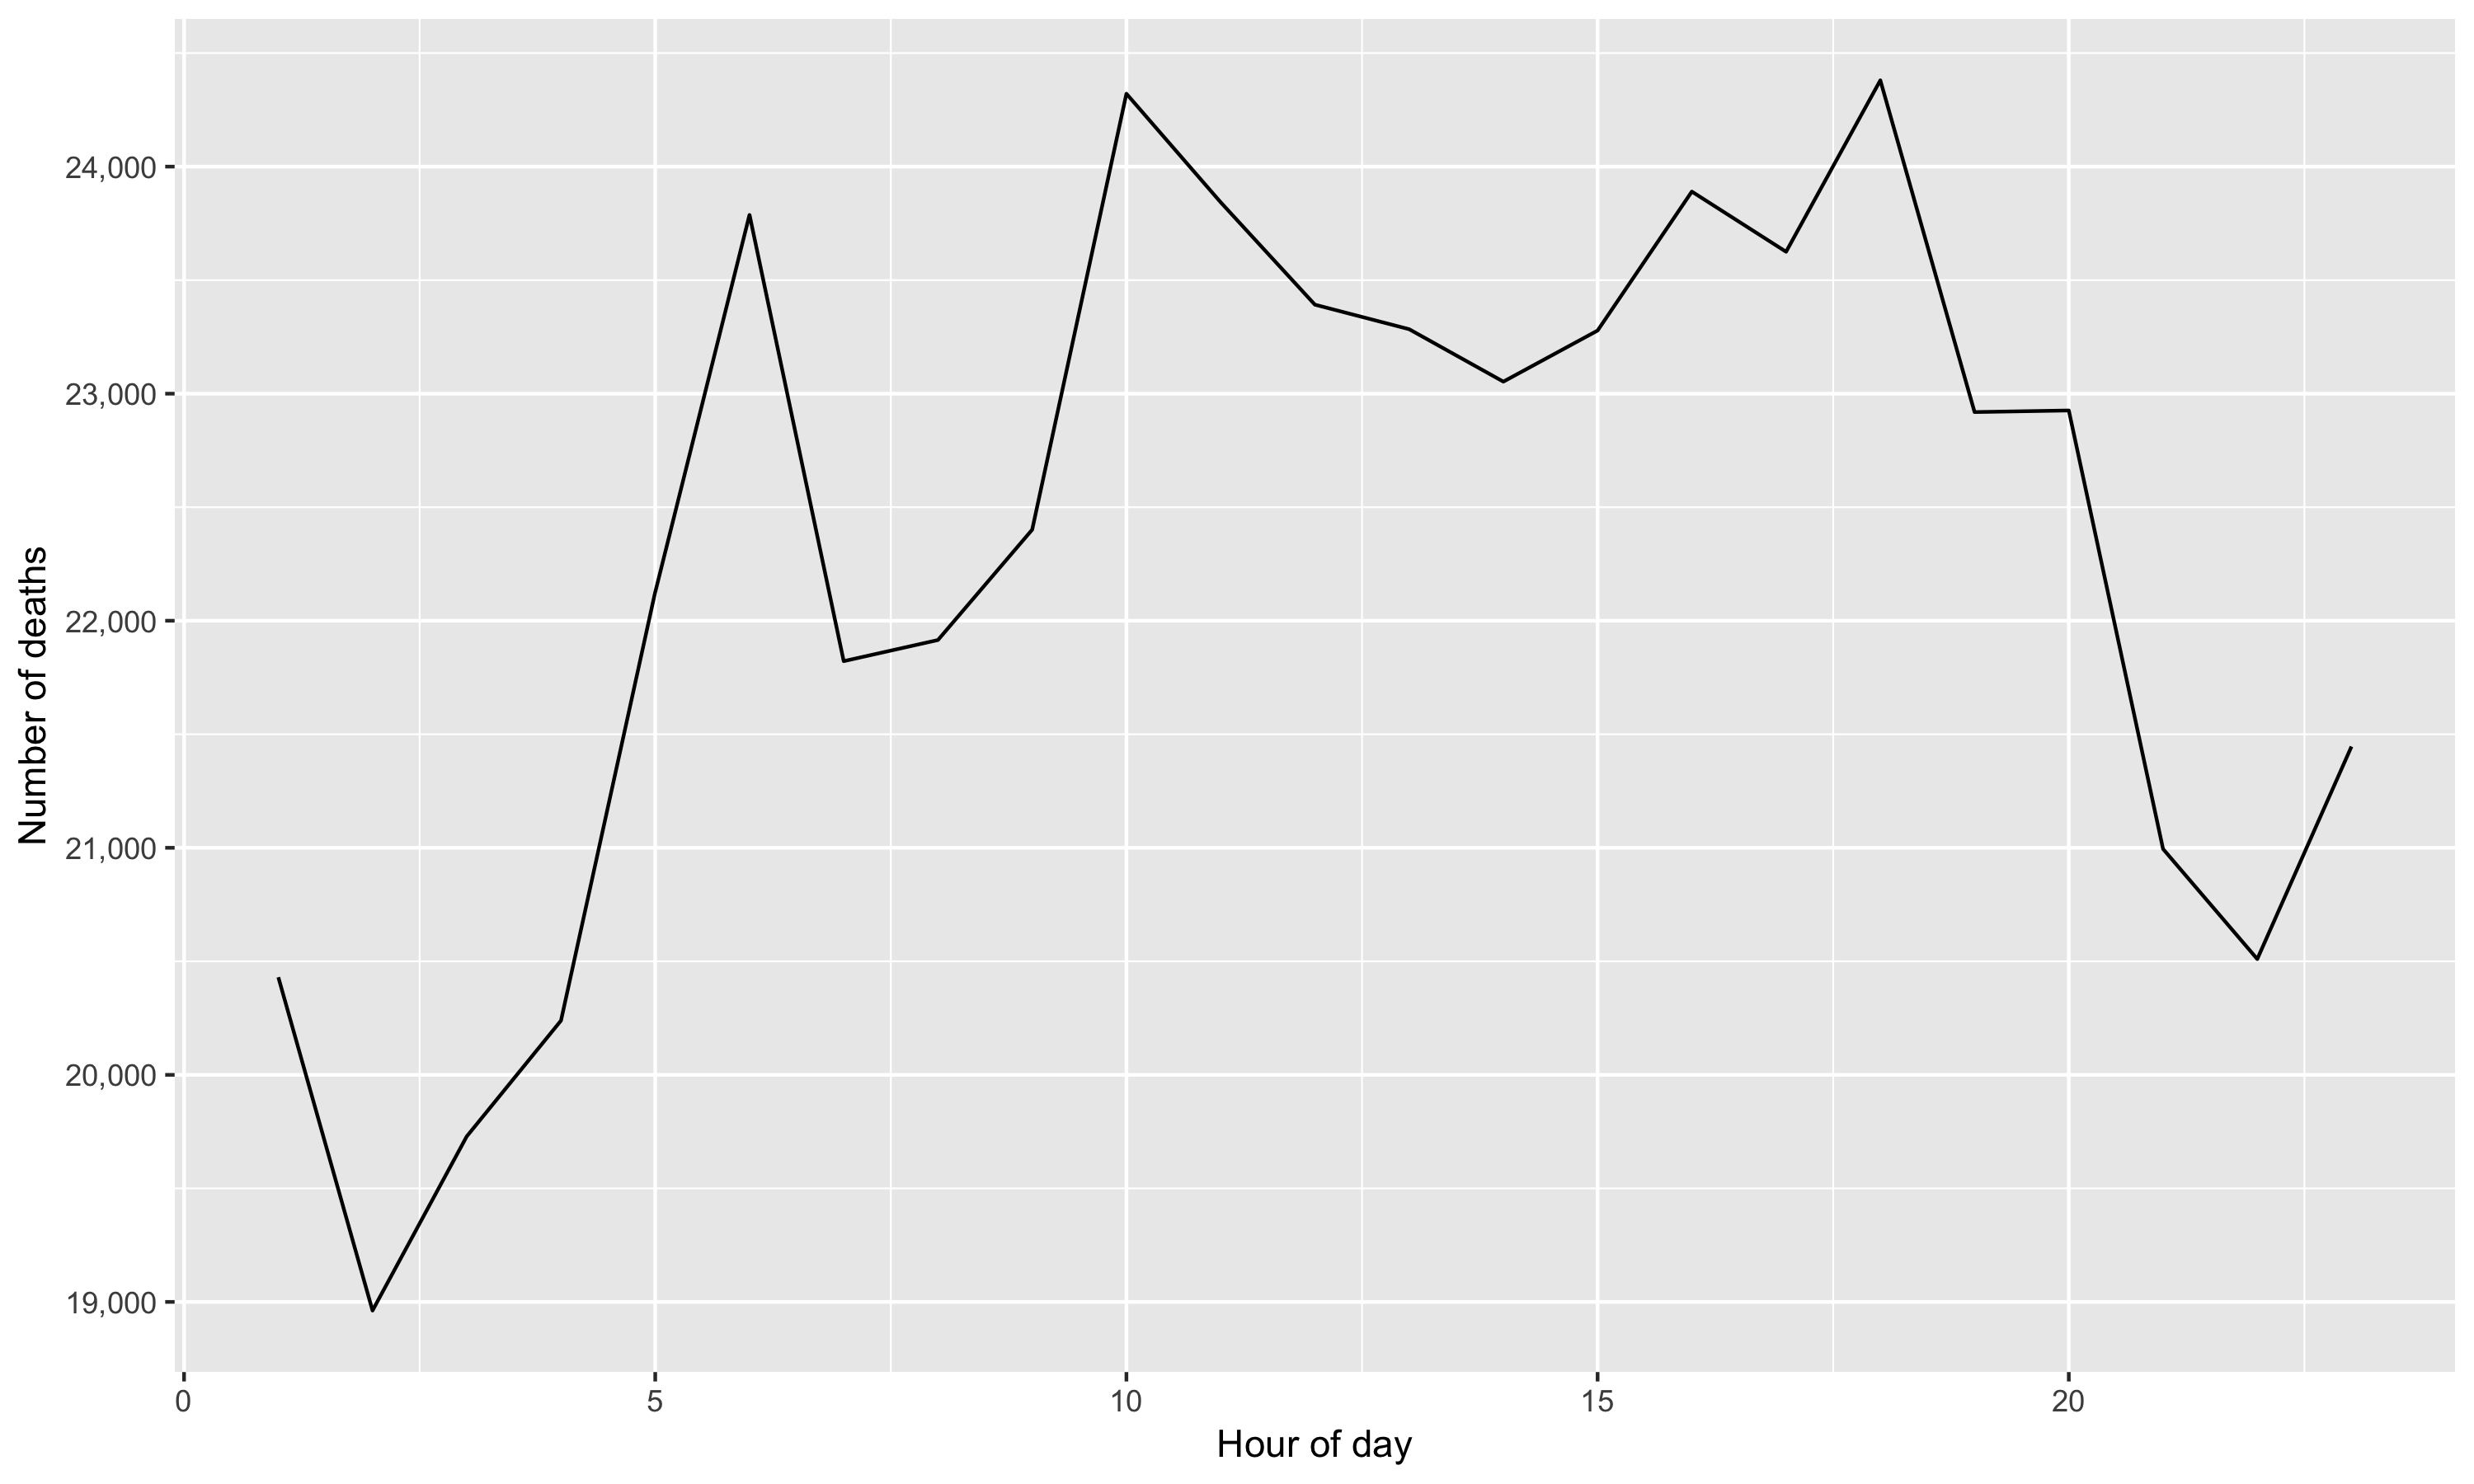
\includegraphics[width=0.9\linewidth]{tidy_case_study/overall} 

}

\caption{Temporal pattern of all causes of death}\label{fig:unnamed-chunk-2}
\end{figure}

Do you find anything unusual or unexpected? The figure shows several
peaks within a day, indicating some increased risks of deaths in certain
times of the day. What would be generating these patterns?

Wickham, the author, finds;

\begin{quote}
The causes of {[}unusual{]} death fall into three main groups: murder,
drowning, and transportation related. Murder is more common at night,
drowning in the afternoon, and transportation related deaths during
commute times \citep{Wickham2014}.
\end{quote}

\begin{figure}
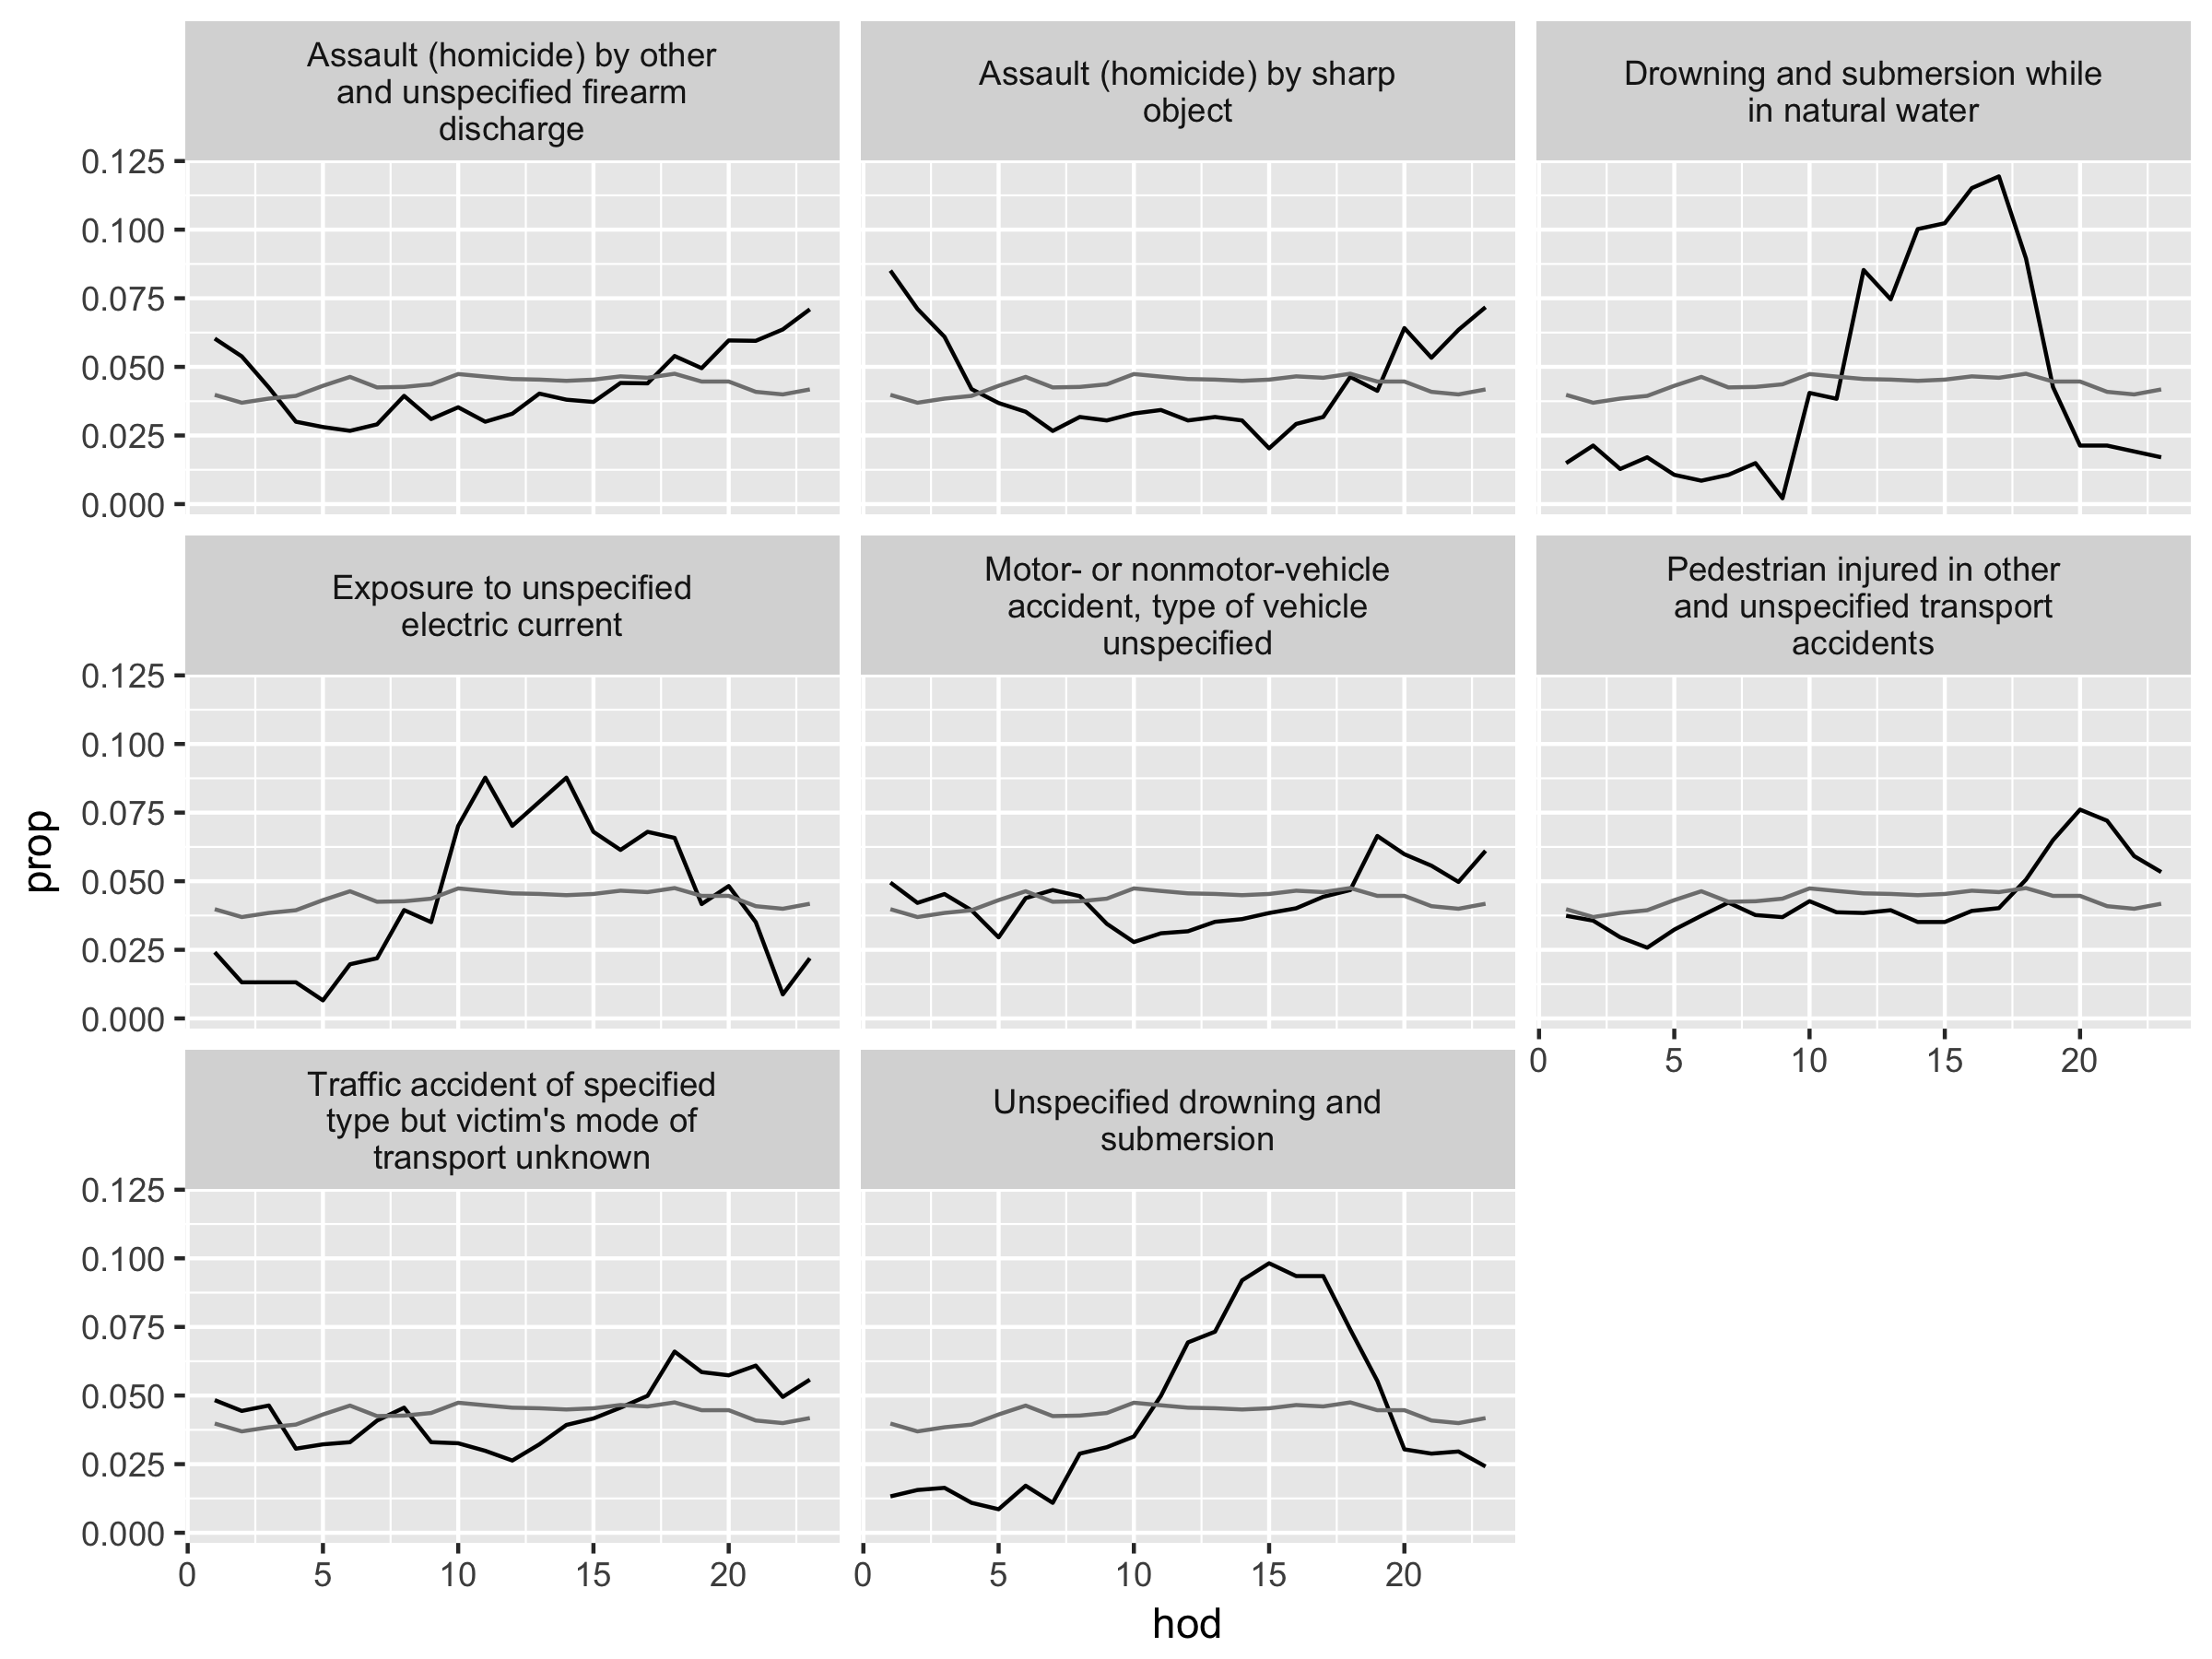
\includegraphics[width=1\linewidth]{tidy_case_study/unusual-big} \caption{Causes of death with unusual temporal courses. Overall hourly death rate shown in grey. Causes of death with more than 350 deaths over a year.}\label{fig:unusual-big}
\end{figure}

We will use two datasets: \texttt{deaths} containing the timing and
coded causes of deaths and \texttt{codes} containing the lookup table
for the coded causes.

The dataset \texttt{deaths} has over 53,000 records (rows), so we use
\texttt{head()} to look at the first several rows.

\begin{Shaded}
\begin{Highlighting}[]
\CommentTok{# "deaths08b" is a renamed dataset with easier-to-read column names }
\KeywordTok{head}\NormalTok{(deaths08b) }
\end{Highlighting}
\end{Shaded}

\begin{verbatim}
##   Year of Death (yod) Month of Death (mod) Day of Death (dod)
## 1                2008                    1                  1
## 2                2008                    1                  1
## 3                2008                    1                  1
## 4                2008                    1                  1
## 5                2008                    1                  1
## 6                2008                    1                  1
##   Hour of Death (hod) Cause of Death (cod)
## 1                   1                  B20
## 2                   1                  B22
## 3                   1                  C18
## 4                   1                  C34
## 5                   1                  C50
## 6                   1                  C50
\end{verbatim}

The dataset \texttt{codes} has 1851 records.

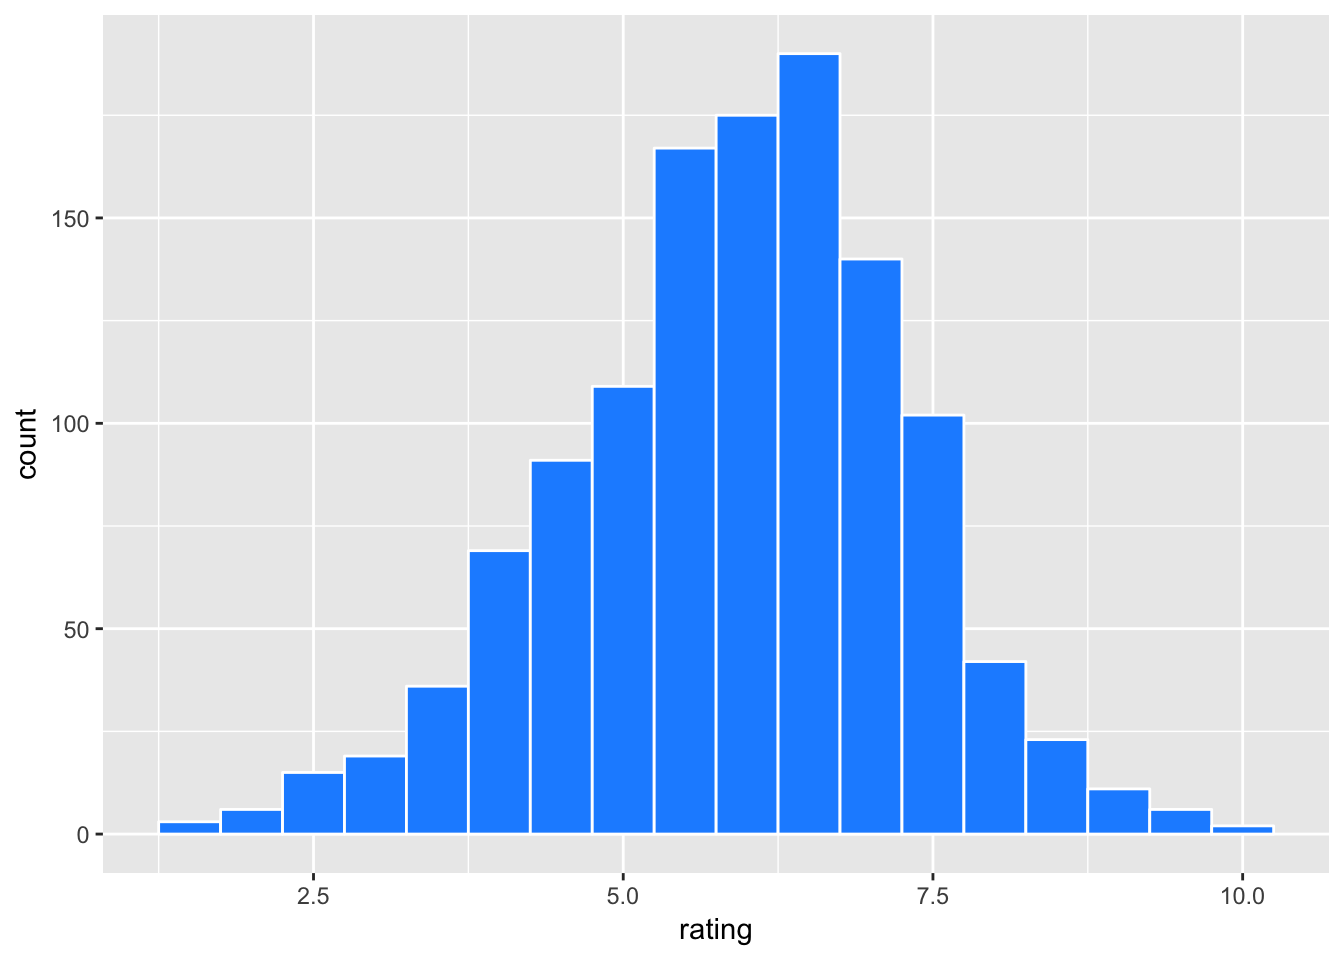
\includegraphics{04-01-tidy-dplyr_files/figure-latex/unnamed-chunk-4-1.pdf}

This table is generated by \href{https://rstudio.github.io/DT/}{DT} and
\href{https://cran.r-project.org/web/packages/webshot/vignettes/intro.html}{webshot}
packages. In the search box, you can type in key words like
``bacteria'', ``nutrition'', and ``fever'', as well as ``assault'' and
``exposure'' to see what items are in the data.

We will reproduce this case study and practice using functions of
\texttt{dplyr} and \texttt{ggplot2}.

\subsection*{Arts \& Crafts}\label{arts-crafts}
\addcontentsline{toc}{subsection}{Arts \& Crafts}

Let's recap key ingredients of
\href{http://docs.ggplot2.org/current/}{dplyr} and
\href{http://docs.ggplot2.org/current/}{ggplot2} from the introduction
in Section \ref{intro}.

The six important functions in \texttt{dplyr} are:

\begin{itemize}
\item
  \texttt{filter()}: extracts rows (e.g., observations) of a data frame.
  We put logical vectors in its arguments.
\item
  \texttt{select()}: extracts columns (e.g., variables) of a data frame.
  We put column names in its arguments.
\item
  \texttt{arrange()}: orders rows of a data frame. We put column names
  in its arguments.
\item
  \texttt{summarise()}: collapses a data frame into summary statistics.
  We put \textbf{summary functions} (e.g., statistics functions) using
  column names in its arguments.
\item
  \texttt{mutate()}: creates new variables and adds them to the existing
  columns. We put \textbf{window functions} (e.g., transforming
  operations) using column names in its arguments.
\item
  \texttt{group\_by()}: assigns rows into groups within a data frame. We
  put column names in its arguments.
\end{itemize}

We use piping operator \texttt{\%\textgreater{}\%} (read as \emph{then})
to translate a sentence of sequential instructions. For example, take
dataset \texttt{deaths08}, \texttt{\%\textgreater{}\%} (\emph{then})
group the data by month of death, and \texttt{\%\textgreater{}\%}
(\emph{then}) summarise the grouped data for the number of observations.

\begin{Shaded}
\begin{Highlighting}[]
\NormalTok{deaths08 %>%}\StringTok{ }
\StringTok{  }\KeywordTok{group_by}\NormalTok{(mod) %>%}\StringTok{   }\CommentTok{# mod: month of death}
\StringTok{  }\KeywordTok{summarise}\NormalTok{( }\DataTypeTok{nobs =} \KeywordTok{n}\NormalTok{() )  }\CommentTok{# n(): a dplyr funciton to count rows }
\end{Highlighting}
\end{Shaded}

\begin{verbatim}
## # A tibble: 12 × 2
##      mod  nobs
##    <int> <int>
## 1      1 49002
## 2      2 41685
## 3      3 44433
## 4      4 39845
## 5      5 41710
## 6      6 38592
## 7      7 40198
## 8      8 40297
## 9      9 39481
## 10    10 41671
## 11    11 43341
## 12    12 42265
\end{verbatim}

The graphics with \texttt{ggplot2} consist of three components:

\begin{itemize}
\item
  \textbf{data}: a data frame e.g., the first argument in
  \texttt{ggplot(data,\ ...)}.
\item
  \textbf{aes}: specifications for x-y variables, as well as variables
  to differentiate \textbf{geom} objects by color , shape, or size.
  e.g., \texttt{aes(x\ =\ var\_x,\ y\ =\ var\_y,\ shape\ =\ var\_z)}
\item
  \textbf{geom}: geometric objects such as points, lines, bars, etc.
  e.g., \texttt{geom\_point()}, \texttt{geom\_line()},
  \texttt{geom\_histogram()}
\end{itemize}

We specify \textbf{data} and \textbf{aes} in \texttt{ggplot()} and then
add \textbf{geom} objects followed by \texttt{+} symbol (read as
\emph{add a layer of}); e.g.,
\texttt{ggplot(data\ =\ dataset,\ mapping\ =\ aes(x\ =\ ...))\ +\ geom\_point()}.
The order of layers added by \texttt{+} symbol is generally
interchangeable.

Combined with \texttt{\%\textgreater{}\%} operator, we can think of the
code as a sentence. For example, take dataset \texttt{deaths08},
\texttt{\%\textgreater{}\%} (\emph{then}) plot with \texttt{gglpot()}
with \texttt{aes()} featuring hour of day on the x-axis, \texttt{+}
(\emph{and add a player of}) geom object \texttt{geom\_histogram()}.

\begin{Shaded}
\begin{Highlighting}[]
\CommentTok{#  a histogram version of the line-graph for the total number of deaths above}
\NormalTok{deaths08 %>%}\StringTok{ }
\StringTok{  }\KeywordTok{ggplot}\NormalTok{(}\KeywordTok{aes}\NormalTok{(}\DataTypeTok{x =} \NormalTok{hod)) +}\StringTok{ }\KeywordTok{geom_histogram}\NormalTok{(}\DataTypeTok{binwidth =} \DecValTok{1}\NormalTok{, }\DataTypeTok{color =} \StringTok{"white"}\NormalTok{) }
\end{Highlighting}
\end{Shaded}

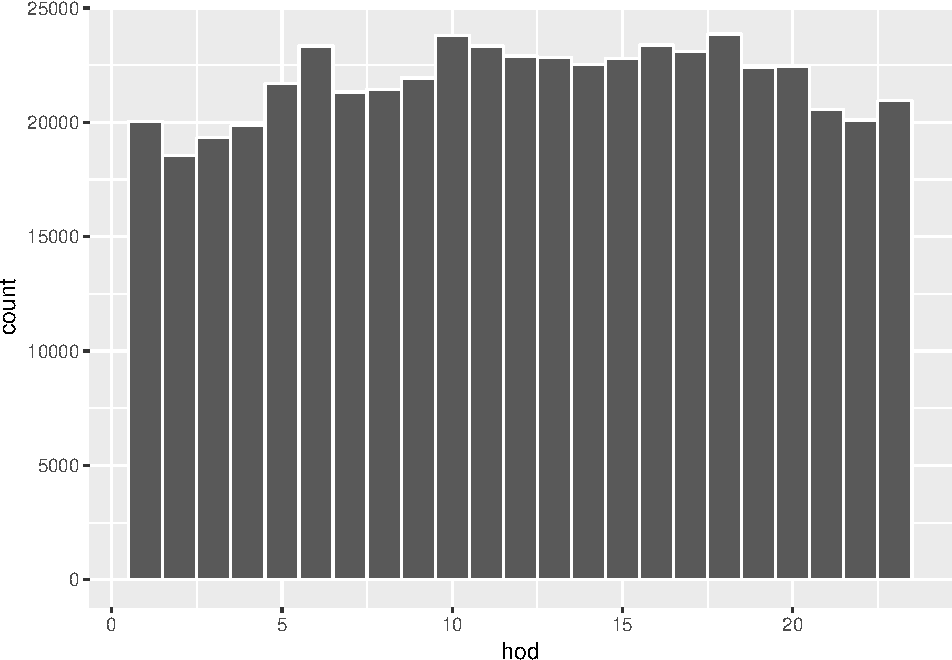
\includegraphics{04-01-tidy-dplyr_files/figure-latex/unnamed-chunk-6-1.pdf}

\begin{Shaded}
\begin{Highlighting}[]
\CommentTok{# a summary by month of day and hour of day.}
\CommentTok{# e.g, Jan-1am, ..,Jan-12pm, Feb-1am,..., Feb-12pm, ...   }
\NormalTok{n_month_hour <-}\StringTok{ }\NormalTok{deaths08 %>%}
\StringTok{  }\KeywordTok{group_by}\NormalTok{(mod, hod) %>%}
\StringTok{  }\KeywordTok{summarise}\NormalTok{( }\DataTypeTok{nobs =} \KeywordTok{n}\NormalTok{() )}

\NormalTok{n_month_hour %>%}
\StringTok{  }\KeywordTok{ggplot}\NormalTok{(}\KeywordTok{aes}\NormalTok{(}\DataTypeTok{x =} \NormalTok{hod, }\DataTypeTok{y =} \NormalTok{nobs, }\DataTypeTok{color =} \KeywordTok{as.factor}\NormalTok{(mod))) +}\StringTok{ }
\StringTok{  }\KeywordTok{geom_point}\NormalTok{() }
\end{Highlighting}
\end{Shaded}

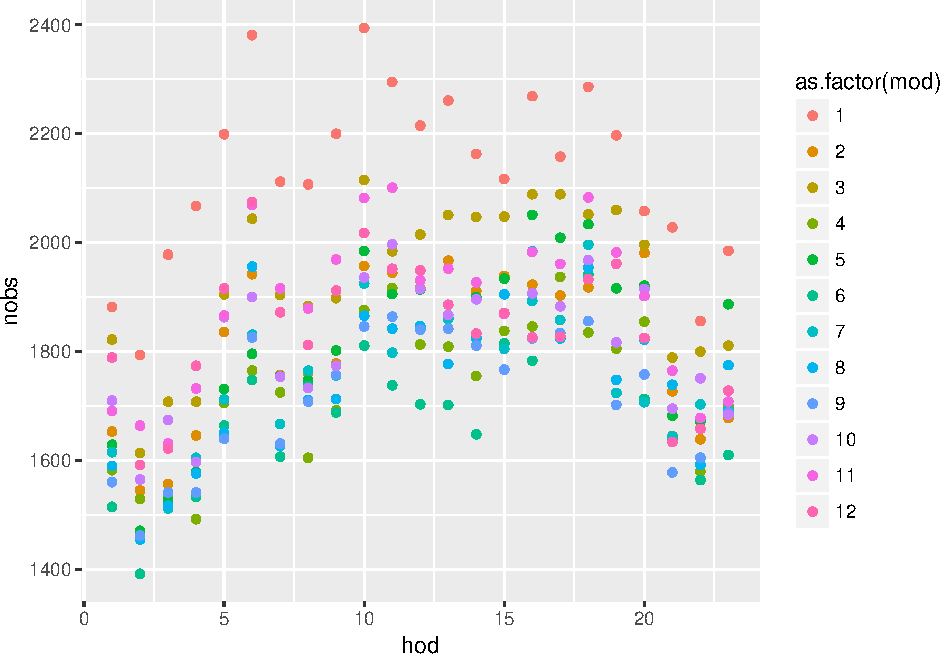
\includegraphics{04-01-tidy-dplyr_files/figure-latex/unnamed-chunk-7-1.pdf}

\begin{Shaded}
\begin{Highlighting}[]
\CommentTok{# "last_plot() + " allows for adding more layers to the previous plot}
\KeywordTok{last_plot}\NormalTok{() +}\StringTok{ }\KeywordTok{geom_line}\NormalTok{()}
\end{Highlighting}
\end{Shaded}

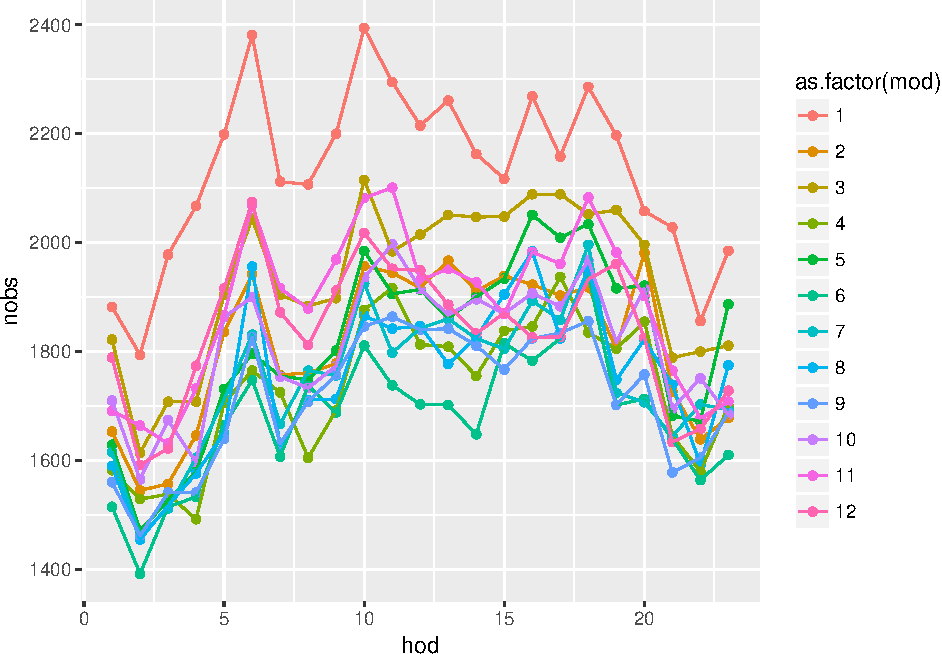
\includegraphics{04-01-tidy-dplyr_files/figure-latex/unnamed-chunk-7-2.pdf}

\subsection*{Exercise}\label{exercise}
\addcontentsline{toc}{subsection}{Exercise}

Now it is your turn. The exercise is to reproduce the above results for
the unusual causes of deaths.

\begin{enumerate}
\def\labelenumi{\arabic{enumi}.}
\item
  Download materials:
  \href{http://vita.had.co.nz/papers/tidy-data.html}{case study paper}
  and
  \href{https://github.com/kotamine/piecemealR/raw/master/tidy_case_study/tidy_case_study.RData}{case
  study data}
\item
  Set working directly: \texttt{setwd(your\_directory)}
\item
  Load libraries: \texttt{library(dplyr)}, \texttt{library(ggplot2)},
  \texttt{library(MASS)} (used for fitting data by robust regression)
\end{enumerate}

\begin{itemize}
\item
  Note 1: There is a minor error in the case study that the author
  accidentally kept several records of data from years other than 2008.
  This virtually has no effect on the results, and we would do the same
  to reproduce the exact results.
\item
  Note 2: You could look at the codes in the paper for hints. However,
  the code is written with the functions of
  \href{https://cran.r-project.org/web/packages/plyr/index.html}{plyr}
  package, or the precesssor of \texttt{dplyr}. Do not load both
  \texttt{plyr} and \texttt{dplyr} libraries in the same R session; they
  do not seem to have good compatibility. Restart R if you accidentally
  loaded both.
\end{itemize}

\subsubsection*{Part A. Display overall hourly
deaths}\label{part-a.-display-overall-hourly-deaths}
\addcontentsline{toc}{subsubsection}{Part A. Display overall hourly
deaths}

We will reproduce:

Hints:

\begin{itemize}
\item
  Filter \texttt{NA} in the hour of day (hod) variable
\item
  Use \texttt{group\_by()}, \texttt{summarise()}, \texttt{n()} to obtain
  death counts by group
\item
  Use \texttt{ggplot()\ +\ geom\_line()} to produce plot
\item
  Use \texttt{+\ labs(\ x\ =\ "x\ lable",\ y\ =\ "y\ label")} for axis
  labels
\item
  see help file of \texttt{scale\_y\_continous()} for comma (use
  \texttt{?function\_name} for help)
\end{itemize}

\subsubsection*{Part B. Count deaths per hour, per
disease}\label{part-b.-count-deaths-per-hour-per-disease}
\addcontentsline{toc}{subsubsection}{Part B. Count deaths per hour, per
disease}

We will reproduce:

\begin{center}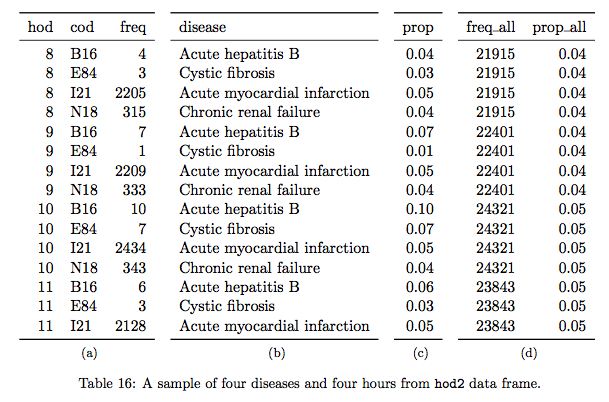
\includegraphics[width=0.9\linewidth]{tidy_case_study/table16} \end{center}

Panel (a) of the table contains the frequency (i.e.~the number of rows)
for each combination of hour of day (hod) and cause of death (cod),
supplemented by the disease description in panel (b). Panel (c) shows
the proportion (prop) of each hod-cod combination in the total deaths by
the cod. Panel (d) contains the frequency and proportion (freq\_all and
prop\_all) of the deaths by hour of day.

That is, panel (a) is the raw counts (e.g., frequency) of observations
by \textbf{each pair} of hour of day (hod) and cause of death (cod), and
panel (b) makes it easy to see the cause of death (cod). Panel (c)
converts this frequency of \emph{hod-cod pair} into the relative
frequency within the total frequency of \textbf{cod}, so that we see at
which \textbf{hour} a disproportinately large number of deaths occurs
for \textbf{cod}. Panel (d), on the other hand, presents the overall
hourly death rates; if every hour has the same probablity of death, we
would see prop\_all \(\approx\) 0.042 (i.e., 1/24). Here, we see the
author's idea of identifying ``unusual deaths'' by comparing ``prop'' of
each \textbf{hod-cod pairs} for the deviation from to ``prop\_all'' (see
figure \ref{fig:unusual-big}).

Hints for creating panels (a)

\begin{itemize}
\item
  Use more than one variable in \texttt{group\_by()}
\item
  Use \texttt{summarise()} with \texttt{n()} to obtain death counts by
  group
\end{itemize}

Hints for creating panels (b)

\begin{itemize}
\tightlist
\item
  Use \texttt{left\_join()} to add the information from dataset
  \texttt{codes}
\end{itemize}

Hints for creating panel (c)

\begin{itemize}
\tightlist
\item
  Use \texttt{mutate()} with \texttt{sum()} on the joined dataset
\end{itemize}

Hints for creating panels (d)

\begin{itemize}
\item
  Create a new data frame by using \texttt{summarise()} on the joined
  and mutated data frame. (\texttt{summarise()} will reduce the
  dimension of the data frame to its summmary, which is the basis of
  panel (d). Once the desired summary is created, merge it to the data
  frame of panels (a)-(c).)
\item
  Before using \texttt{summarise()} above, use \texttt{group\_by()} to
  specify new grouping
\item
  First create \texttt{freq\_all} variable via \texttt{summarise()} with
  \texttt{n()} and then create \texttt{prop\_all} variable via
  \texttt{mutate()} with \texttt{sum()} (call this data frame
  \texttt{overall\_freq}, which will be used again at the very end)
\item
  Use \texttt{left\_join()} to join panels (a)-(c) and panel (d)
  (\texttt{overall\_freq}), which we refer to as \texttt{master\_hod}
  data frame.
\end{itemize}

Hints for extracting the same rows as in the Table 16 above

\begin{itemize}
\item
  Create a subset of the \texttt{master\_hod} data under a new name
\item
  Use \texttt{filter()} to select \texttt{cod} being either ``I21'',
  ``N18'', ``E84'', or ``B16'' and \texttt{hod} being greater or equal
  to 8 and smaller or less than 11
\item
  Use \texttt{select()} to pick columns in a desired order and
  \texttt{arrange()} to sort
\end{itemize}

\subsubsection*{Part C. Find outliers}\label{part-c.-find-outliers}
\addcontentsline{toc}{subsubsection}{Part C. Find outliers}

We will reproduce:

\begin{center}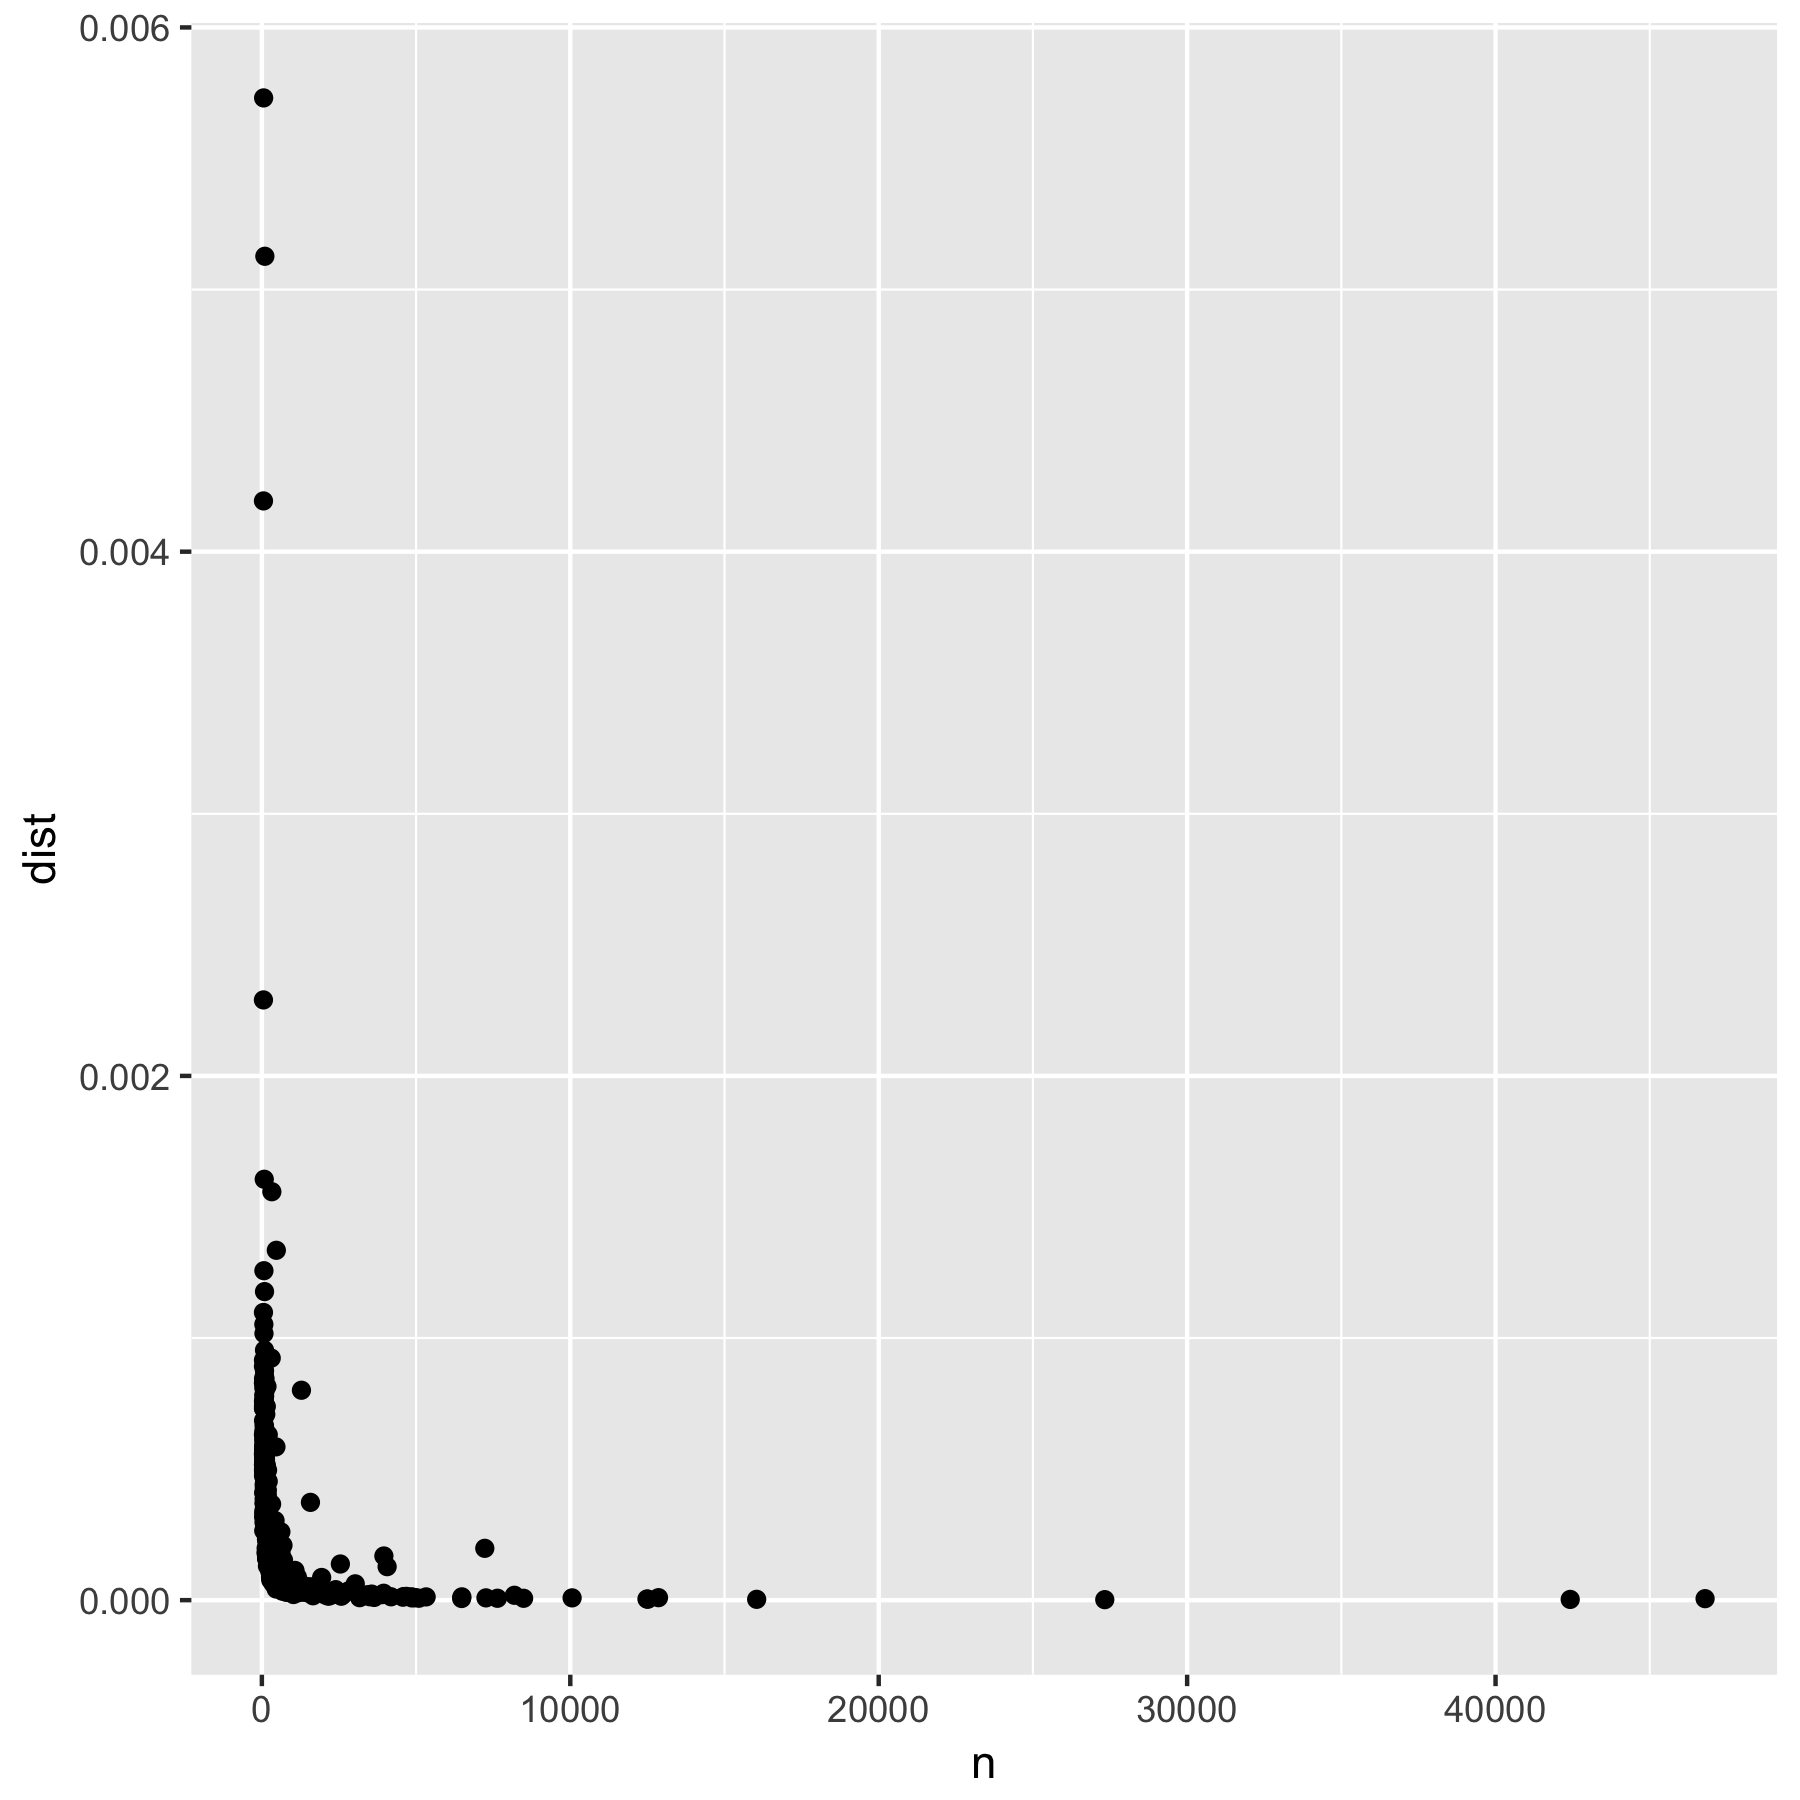
\includegraphics[width=0.5\linewidth]{tidy_case_study/n-dist-raw} \end{center}

\begin{center}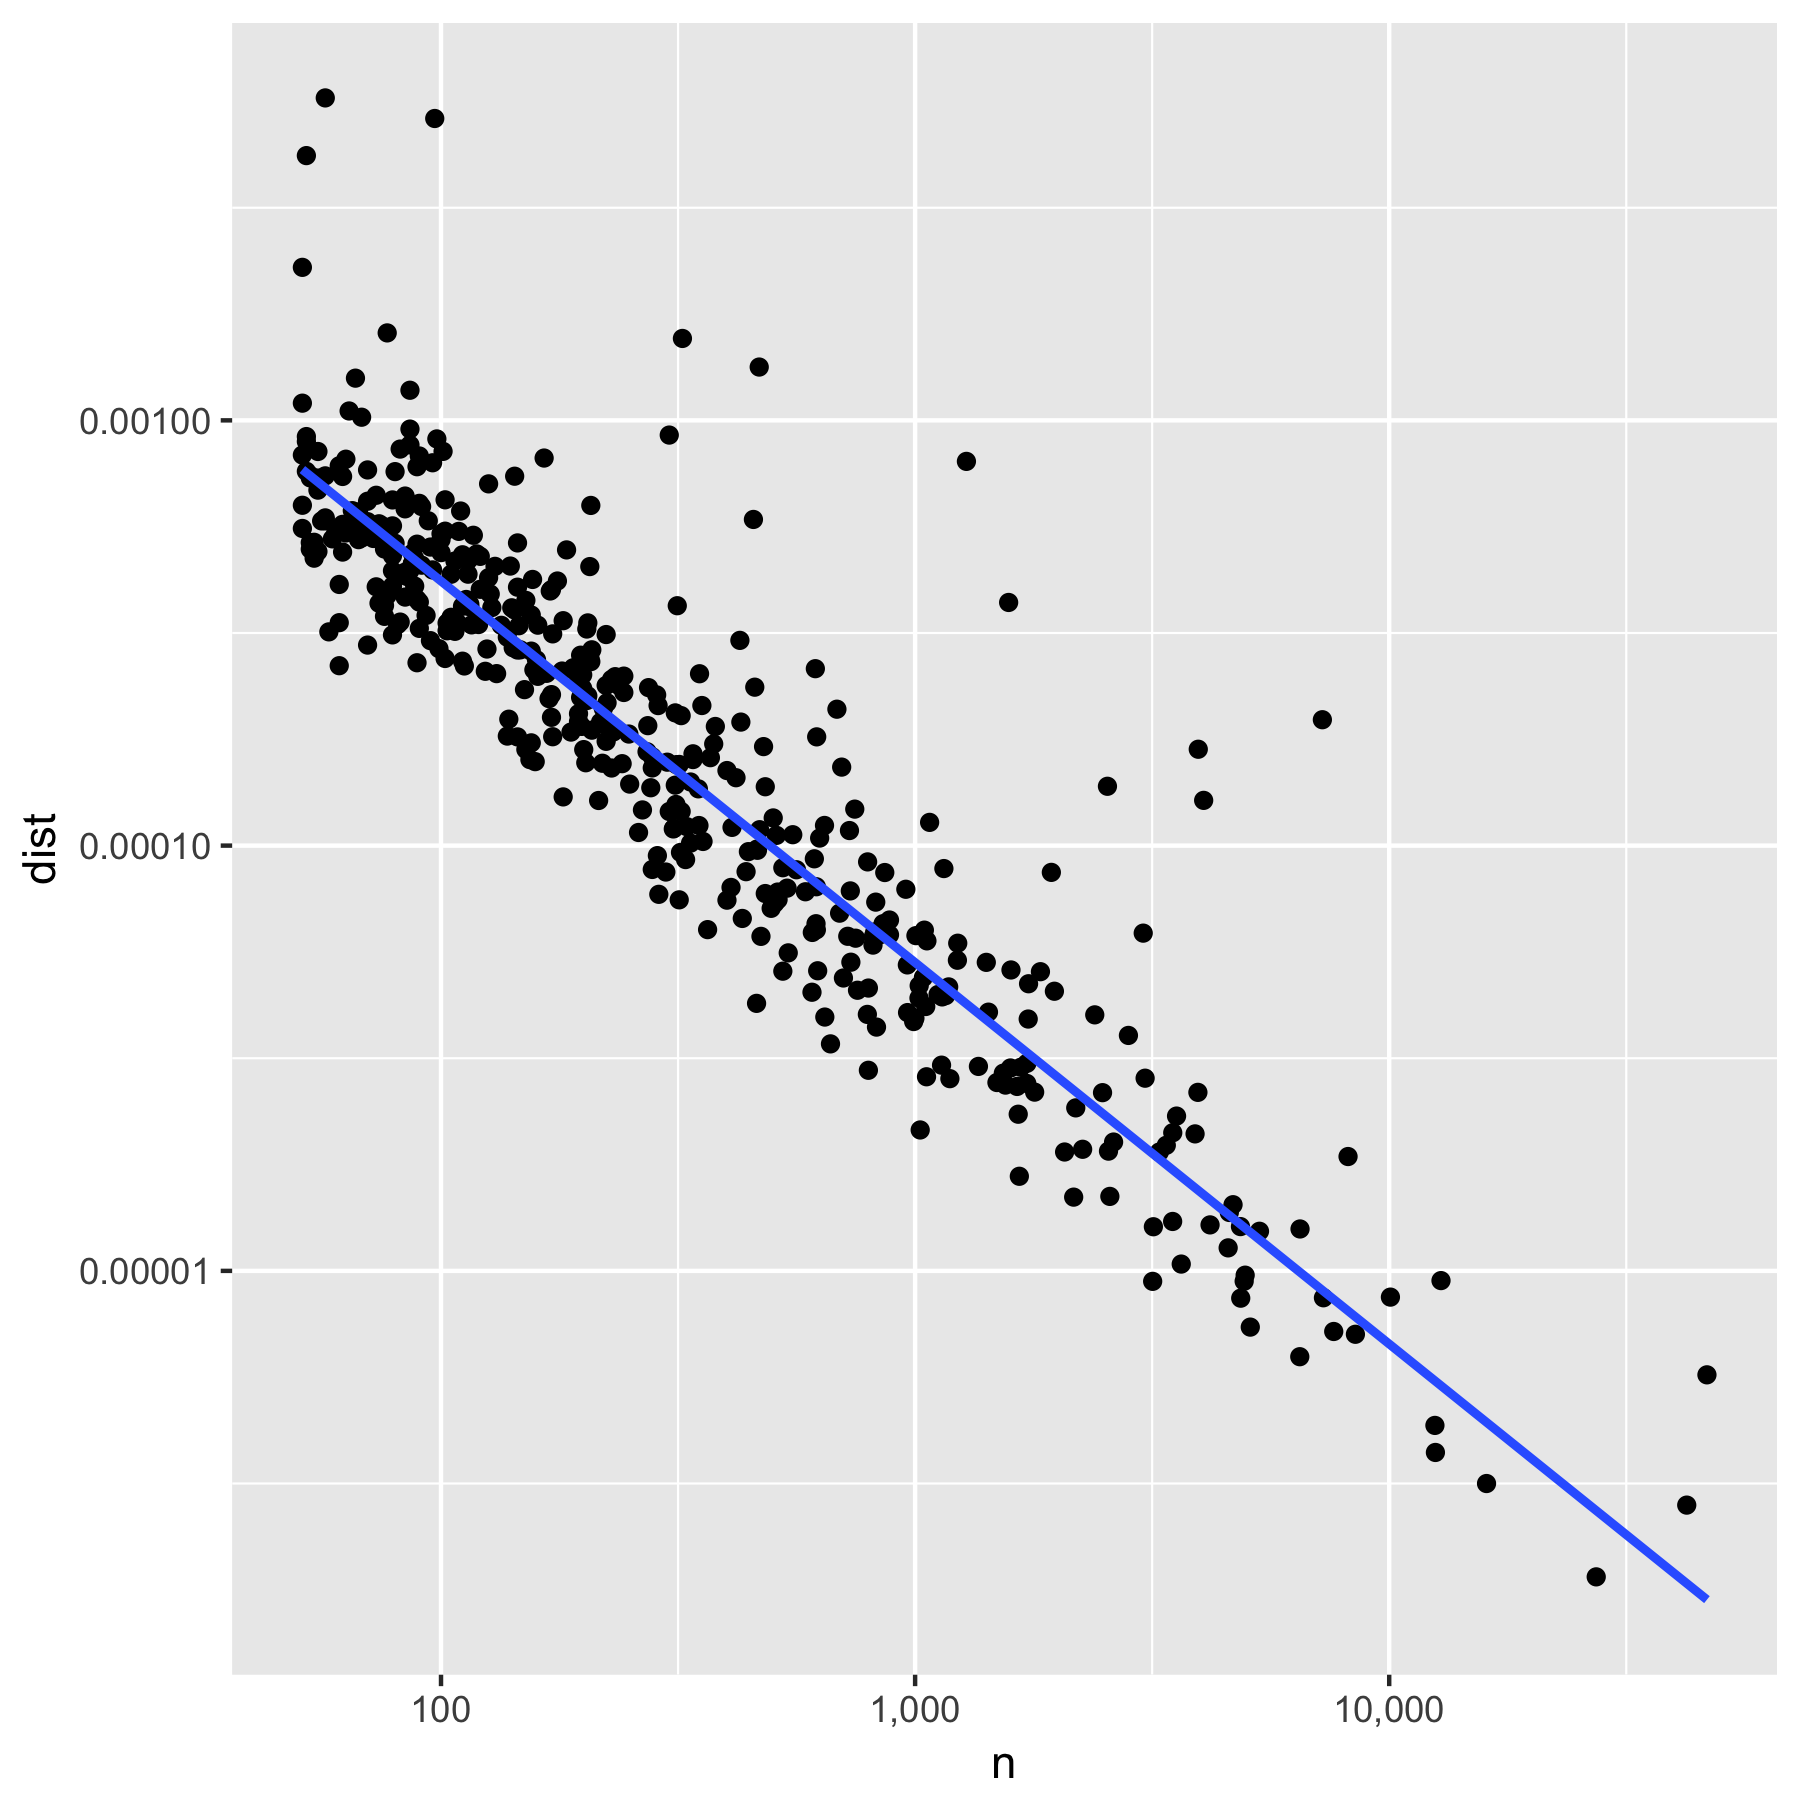
\includegraphics[width=0.5\linewidth]{tidy_case_study/n-dist-log} \end{center}

We will create a deviation variable named \texttt{dist} by taking the
mean of squared differences between \texttt{prop} and
\texttt{prop\_all}. The above figures show the the number of
observations \texttt{n} and this distance measure \texttt{dist} by cause
of death in the raw scale (left) and in the log scale (right).

Hints

\begin{itemize}
\item
  Use \texttt{group\_by()} and \texttt{summarise()} on the
  \texttt{master\_hod} data frame to generate \texttt{n} with function
  \texttt{sum()} and \texttt{dist} by
  \texttt{mean((prop\ -\ prop\_all)\^{}2)}
\item
  Filter this summary for \texttt{n\ \textgreater{}\ 50} and call it
  \texttt{devi\_cod} (deviations by cause of death)
\item
  Use \texttt{ggplot()\ +\ geom\_point()} with
  \texttt{data\ =\ devi\_cod} to produce the raw-scale figure
\item
  Additionally use \texttt{scale\_x\_log10()},
  \texttt{scale\_y\_log10()}, and
  \texttt{geom\_smooth(method\ =\ "rlm",\ se\ =\ FALSE)} to produce the
  log-scale figure
\item
  See help for \texttt{scale\_x\_log10()} to adjust axis labels (look
  for ``comma'')
\item
  Technically speaking, we should change the axis labels to indicate the
  logarithmic transformation, but we skip it here.
\item
  Let's not worry about reproducing the exact grids as they appear in
  the paper
\end{itemize}

\subsubsection*{Part D. Fit data by a regression and plot
residuals}\label{part-d.-fit-data-by-a-regression-and-plot-residuals}
\addcontentsline{toc}{subsubsection}{Part D. Fit data by a regression
and plot residuals}

We will reproduce:

\begin{center}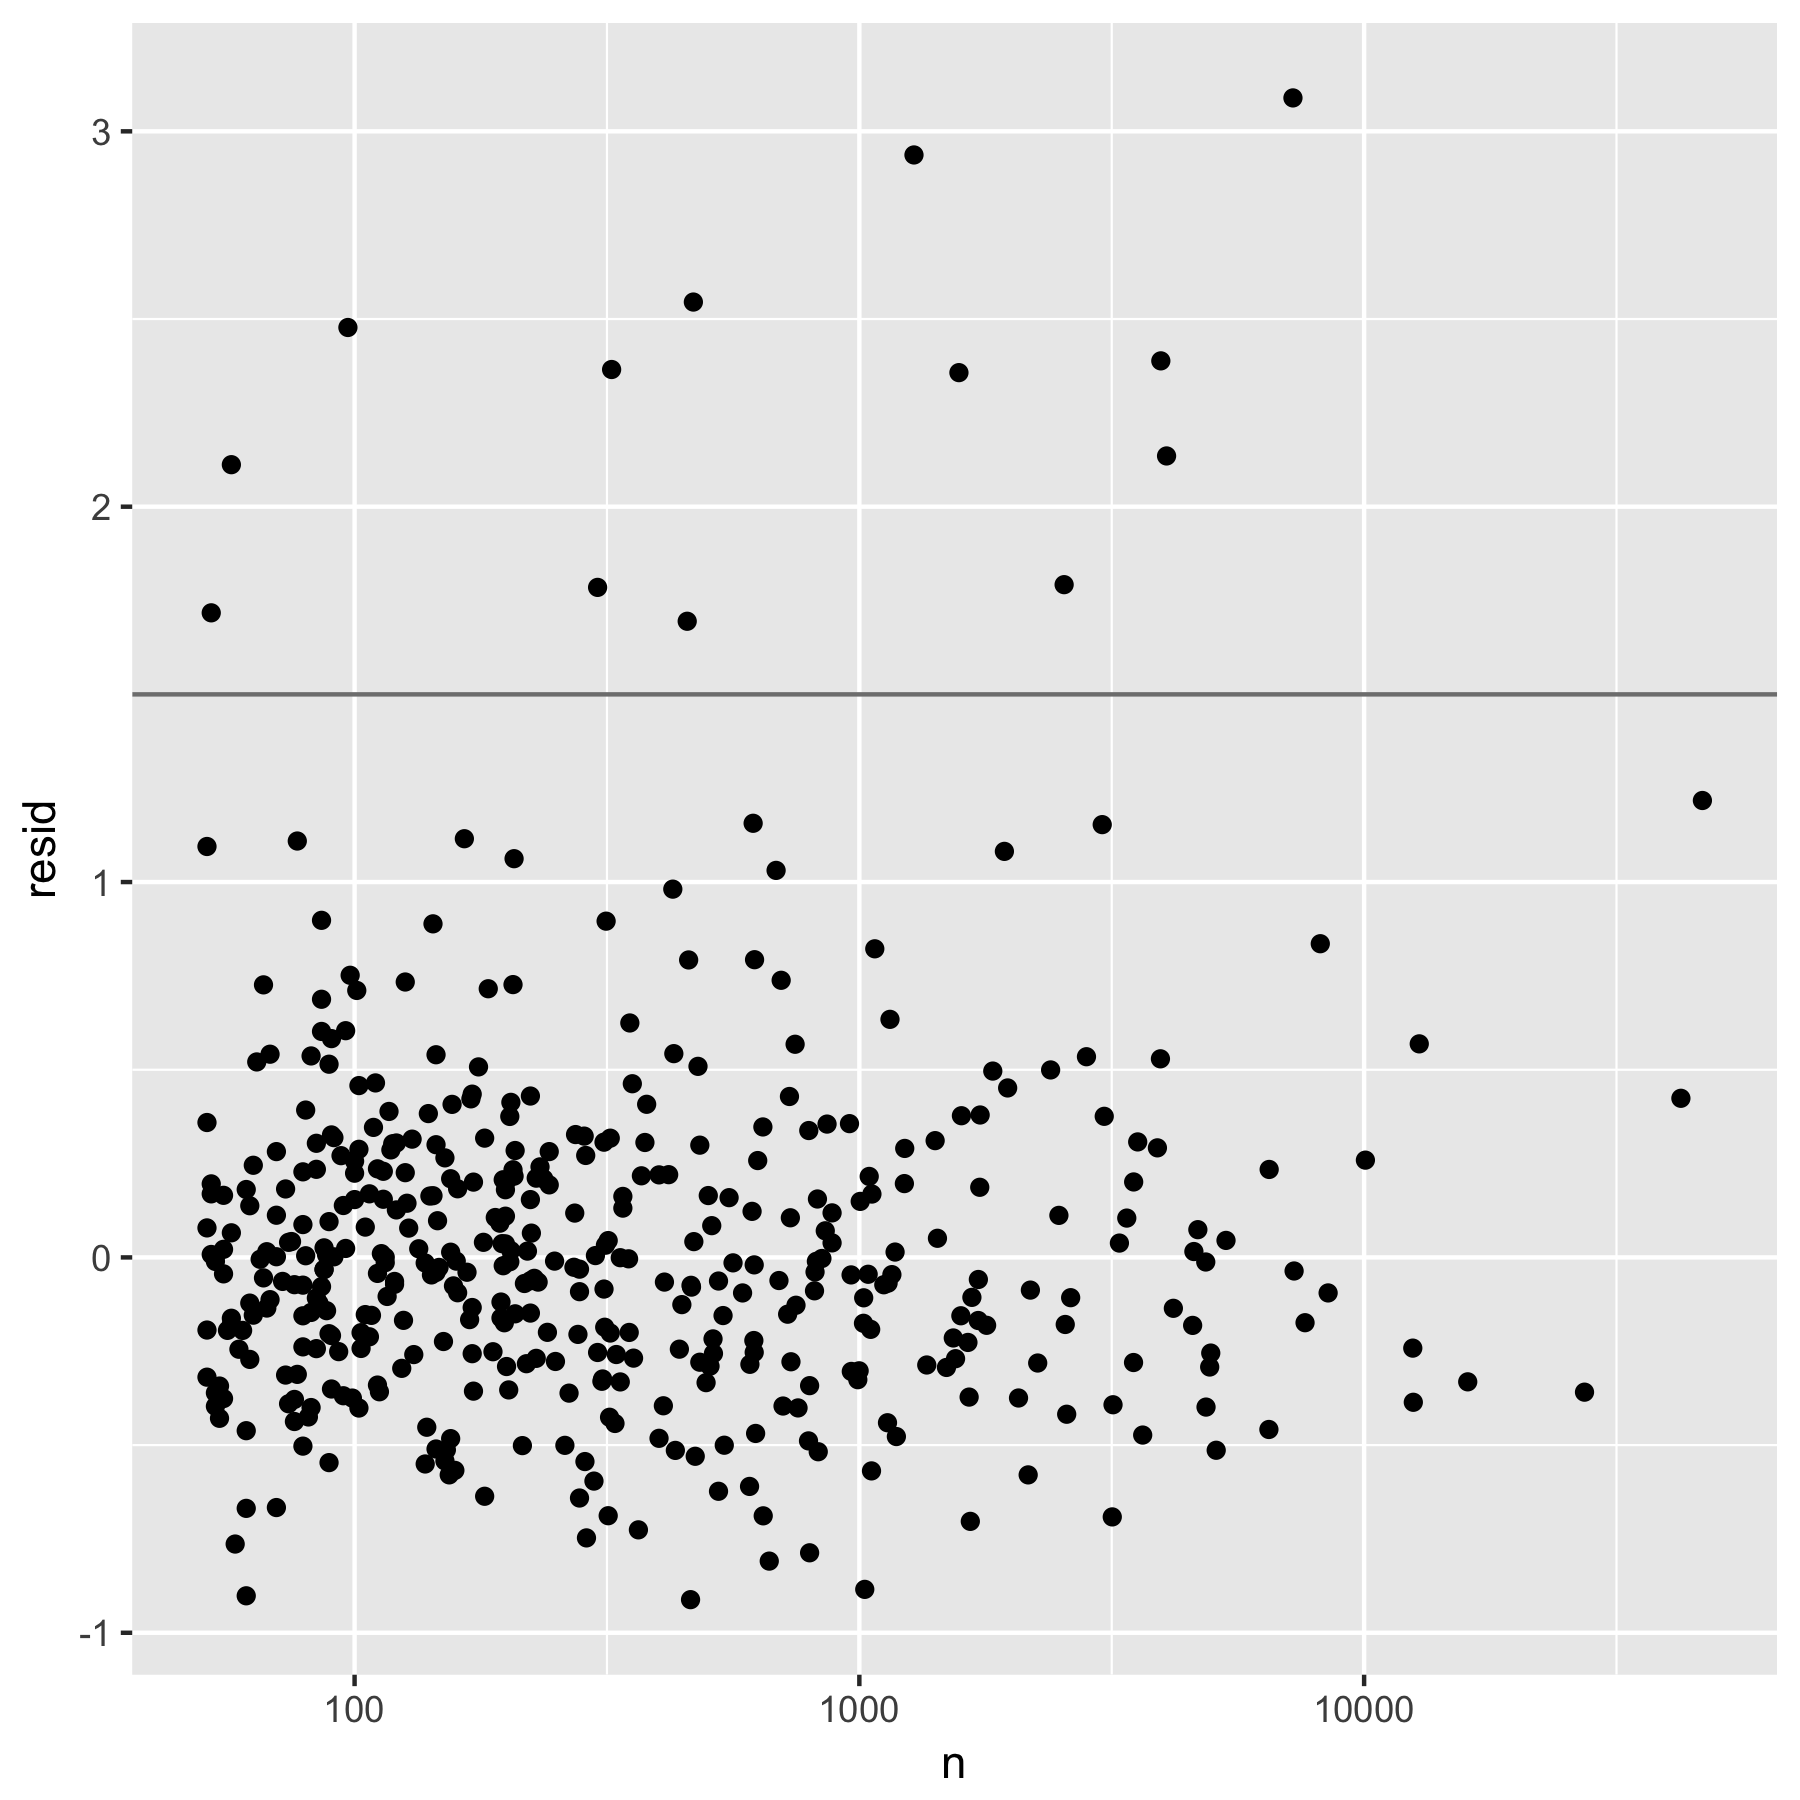
\includegraphics[width=0.5\linewidth]{tidy_case_study/n-dist-resid} \end{center}

The figure is a plot of the regression residuals \texttt{resid} of
\texttt{log(dist)} on \texttt{log(n)}. By visual inspection, the points
lying above the holizontal line at \texttt{resid=1.5} are considered to
be ``unusual causes of deaths'' by the author.

Here the author used the robust linear model (\texttt{rlm()})
regression, but the syntax is mostly the same as that of the standard
linear model regression (\texttt{lm()} ).

Here is an example of regression by \texttt{lm()}.

\begin{Shaded}
\begin{Highlighting}[]
\NormalTok{df <-}\StringTok{ }\KeywordTok{data.frame}\NormalTok{(}
  \NormalTok{x1 <-}\StringTok{  }\KeywordTok{c}\NormalTok{(}\DecValTok{1}\NormalTok{:}\DecValTok{10}\NormalTok{),}
  \NormalTok{y1 <-}\StringTok{  }\KeywordTok{c}\NormalTok{(}\DecValTok{1}\NormalTok{,}\DecValTok{3}\NormalTok{,}\DecValTok{2}\NormalTok{,}\DecValTok{4}\NormalTok{,}\DecValTok{6}\NormalTok{,}\DecValTok{5}\NormalTok{,}\DecValTok{7}\NormalTok{,}\DecValTok{5}\NormalTok{,}\DecValTok{7}\NormalTok{,}\DecValTok{8}\NormalTok{)}
\NormalTok{)}

\NormalTok{df %>%}\StringTok{ }
\StringTok{  }\KeywordTok{ggplot}\NormalTok{(}\KeywordTok{aes}\NormalTok{(}\DataTypeTok{x =} \NormalTok{x1, }\DataTypeTok{y =} \NormalTok{y1)) +}\StringTok{ }\KeywordTok{geom_point}\NormalTok{() +}
\StringTok{  }\KeywordTok{geom_smooth}\NormalTok{(}\DataTypeTok{method =} \StringTok{"lm"}\NormalTok{, }\DataTypeTok{se =} \OtherTok{FALSE}\NormalTok{)}
\end{Highlighting}
\end{Shaded}

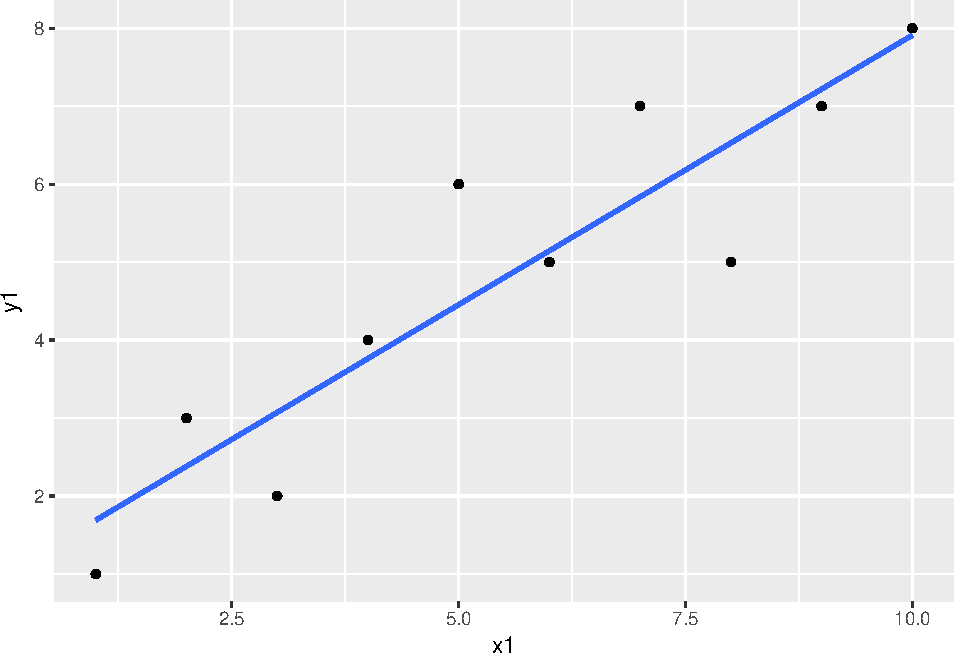
\includegraphics{04-01-tidy-dplyr_files/figure-latex/unnamed-chunk-11-1.pdf}

The geom\_smooth() is estimating the following linear regression:
\[ y1 = intercept + coefficient * x1 + residual\] The model is estimated
by \texttt{lm()} as follows;

\begin{Shaded}
\begin{Highlighting}[]
\NormalTok{f1 <-}\StringTok{ }\KeywordTok{lm}\NormalTok{(}\DataTypeTok{formula =} \NormalTok{y1 ~}\StringTok{ }\NormalTok{x1,  }\DataTypeTok{data =} \NormalTok{df) }
\end{Highlighting}
\end{Shaded}

Now let's see what we get out of the estimation results \texttt{f1}.

\begin{Shaded}
\begin{Highlighting}[]
\KeywordTok{class}\NormalTok{(f1)    }\CommentTok{# class "lm"}
\end{Highlighting}
\end{Shaded}

\begin{verbatim}
## [1] "lm"
\end{verbatim}

\begin{Shaded}
\begin{Highlighting}[]
\KeywordTok{summary}\NormalTok{(f1)  }\CommentTok{# summary() knows how to summarise an object of class "lm" }
\end{Highlighting}
\end{Shaded}

\begin{verbatim}
## 
## Call:
## lm(formula = y1 ~ x1, data = df)
## 
## Residuals:
##      Min       1Q   Median       3Q      Max 
## -1.52727 -0.57273 -0.02727  0.52273  1.54545 
## 
## Coefficients:
##             Estimate Std. Error t value Pr(>|t|)    
## (Intercept)   1.0000     0.6924   1.444 0.186656    
## x1            0.6909     0.1116   6.192 0.000262 ***
## ---
## Signif. codes:  0 '***' 0.001 '**' 0.01 '*' 0.05 '.' 0.1 ' ' 1
## 
## Residual standard error: 1.014 on 8 degrees of freedom
## Multiple R-squared:  0.8273, Adjusted R-squared:  0.8058 
## F-statistic: 38.34 on 1 and 8 DF,  p-value: 0.0002618
\end{verbatim}

\begin{Shaded}
\begin{Highlighting}[]
\KeywordTok{coefficients}\NormalTok{(f1)  }\CommentTok{# coefficient point estimate}
\end{Highlighting}
\end{Shaded}

\begin{verbatim}
## (Intercept)          x1 
##   1.0000000   0.6909091
\end{verbatim}

\begin{Shaded}
\begin{Highlighting}[]
\KeywordTok{vcov}\NormalTok{(f1)          }\CommentTok{# coefficient variance-covariance matrix}
\end{Highlighting}
\end{Shaded}

\begin{verbatim}
##             (Intercept)          x1
## (Intercept)  0.47939394 -0.06848485
## x1          -0.06848485  0.01245179
\end{verbatim}

\begin{Shaded}
\begin{Highlighting}[]
\KeywordTok{predict}\NormalTok{(f1)       }\CommentTok{# predicted (fitted) values with the estimated coefficients }
\end{Highlighting}
\end{Shaded}

\begin{verbatim}
##        1        2        3        4        5        6        7        8 
## 1.690909 2.381818 3.072727 3.763636 4.454545 5.145455 5.836364 6.527273 
##        9       10 
## 7.218182 7.909091
\end{verbatim}

\begin{Shaded}
\begin{Highlighting}[]
\KeywordTok{resid}\NormalTok{(f1)         }\CommentTok{# residuals:  }
\end{Highlighting}
\end{Shaded}

\begin{verbatim}
##           1           2           3           4           5           6 
## -0.69090909  0.61818182 -1.07272727  0.23636364  1.54545455 -0.14545455 
##           7           8           9          10 
##  1.16363636 -1.52727273 -0.21818182  0.09090909
\end{verbatim}

Now let's get back to our exercise and reproduce the figure above.

Hints

\begin{itemize}
\item
  Run a regression by \texttt{rlm} with
  \texttt{formula\ =\ log(dist)\ \textasciitilde{}\ log(n)} and store
  the residuals in \texttt{devi\_cod} data. To read more about linear
  regressions, see the help file of \texttt{lm()} (type \texttt{?lm}).
  For adding a column of residuals, you can use assignment
  \texttt{devi\_cod\$resid\ \textless{}-\ your\_residuals}.
\item
  Plot the residual against log-scale \texttt{n}
\item
  Note: Check the dataset \texttt{devi\_cod} for missing values of
  \texttt{dist} and \texttt{n} before running a regression (you should
  not have missing values in this case). Most regression functions,
  including \texttt{lm()} and \texttt{rlm()}, drop any row with missing
  values from the estimation. This becomes an issue if we want to add a
  new column containing predicted values or residuals to the original
  dataset. (When rows containing missing values are dropped, the vector
  generated by \texttt{predict()} or \texttt{resid()} will be shorter
  than the number of rows in the original dataset.)
\item
  Use \texttt{ggplot()\ +\ geom\_point()} structure for the plot
\item
  Add \texttt{+\ scale\_x\_log10()} and
  \texttt{+\ geom\_hline(yintercept\ =\ 1.5)}
\end{itemize}

\subsubsection*{Part E. Visualise unusual causes of
death}\label{part-e.-visualise-unusual-causes-of-death}
\addcontentsline{toc}{subsubsection}{Part E. Visualise unusual causes of
death}

We will reproduce:

\begin{center}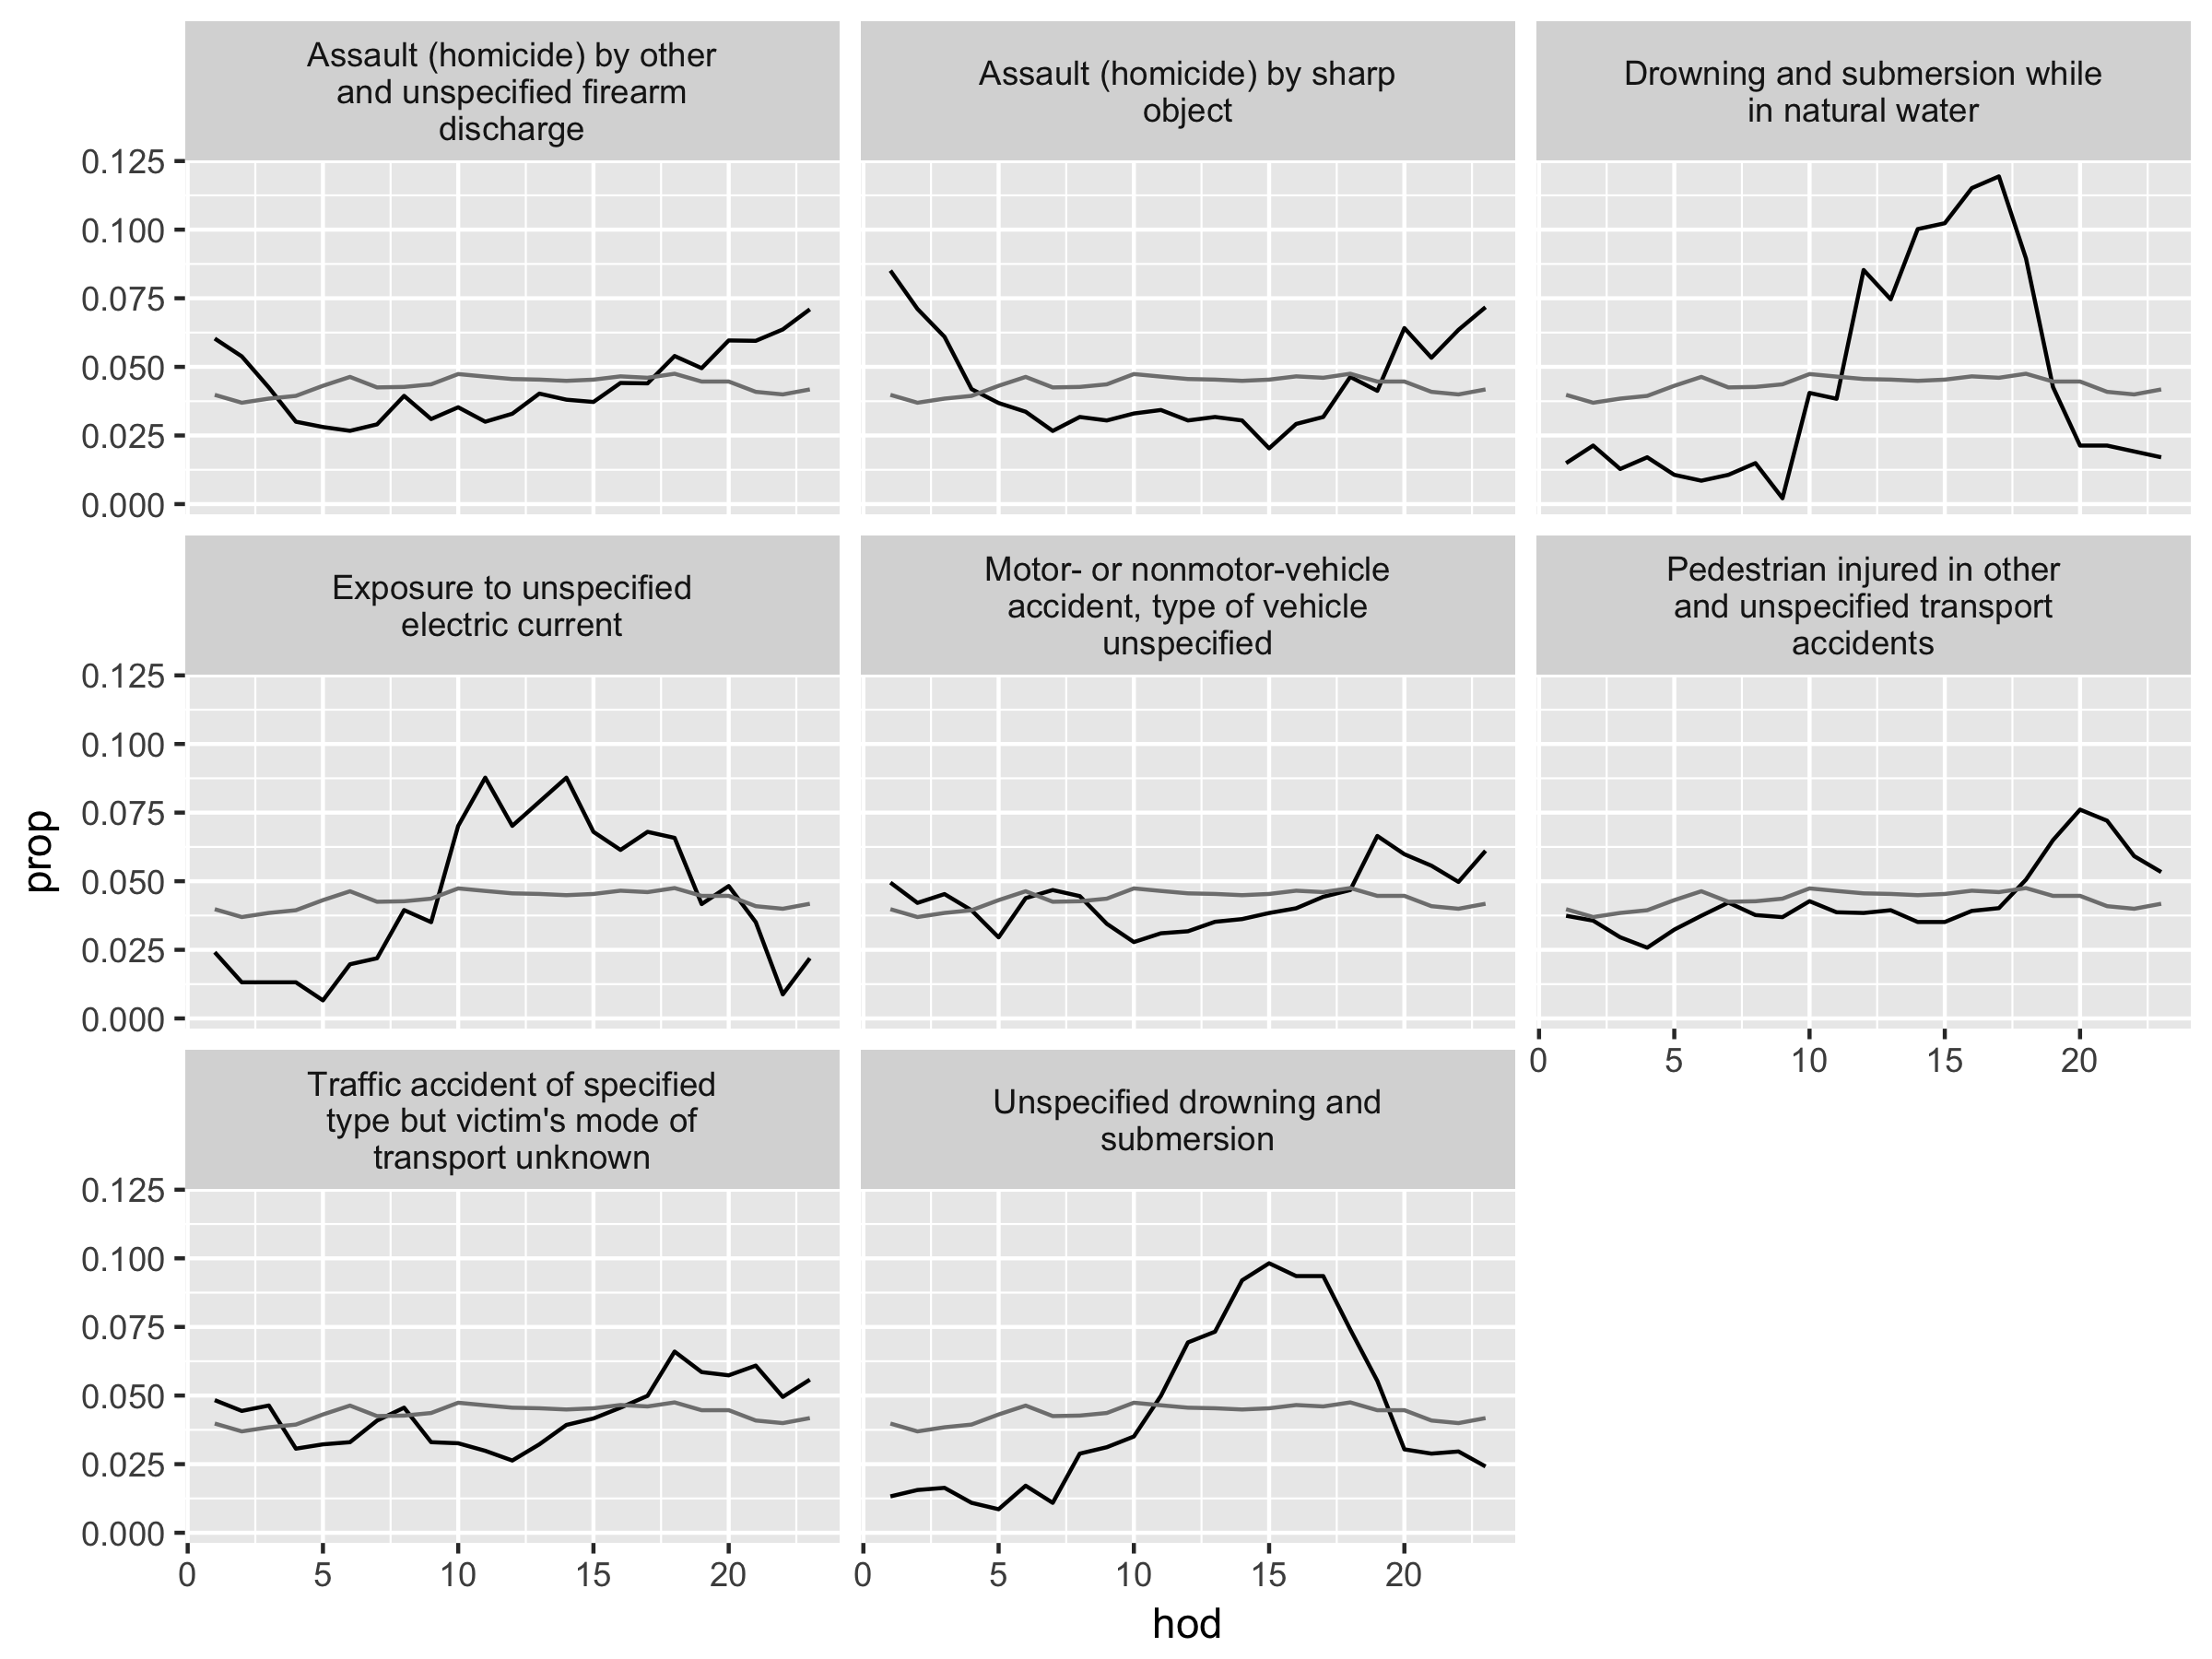
\includegraphics[width=1\linewidth]{tidy_case_study/unusual-big} \end{center}

\begin{center}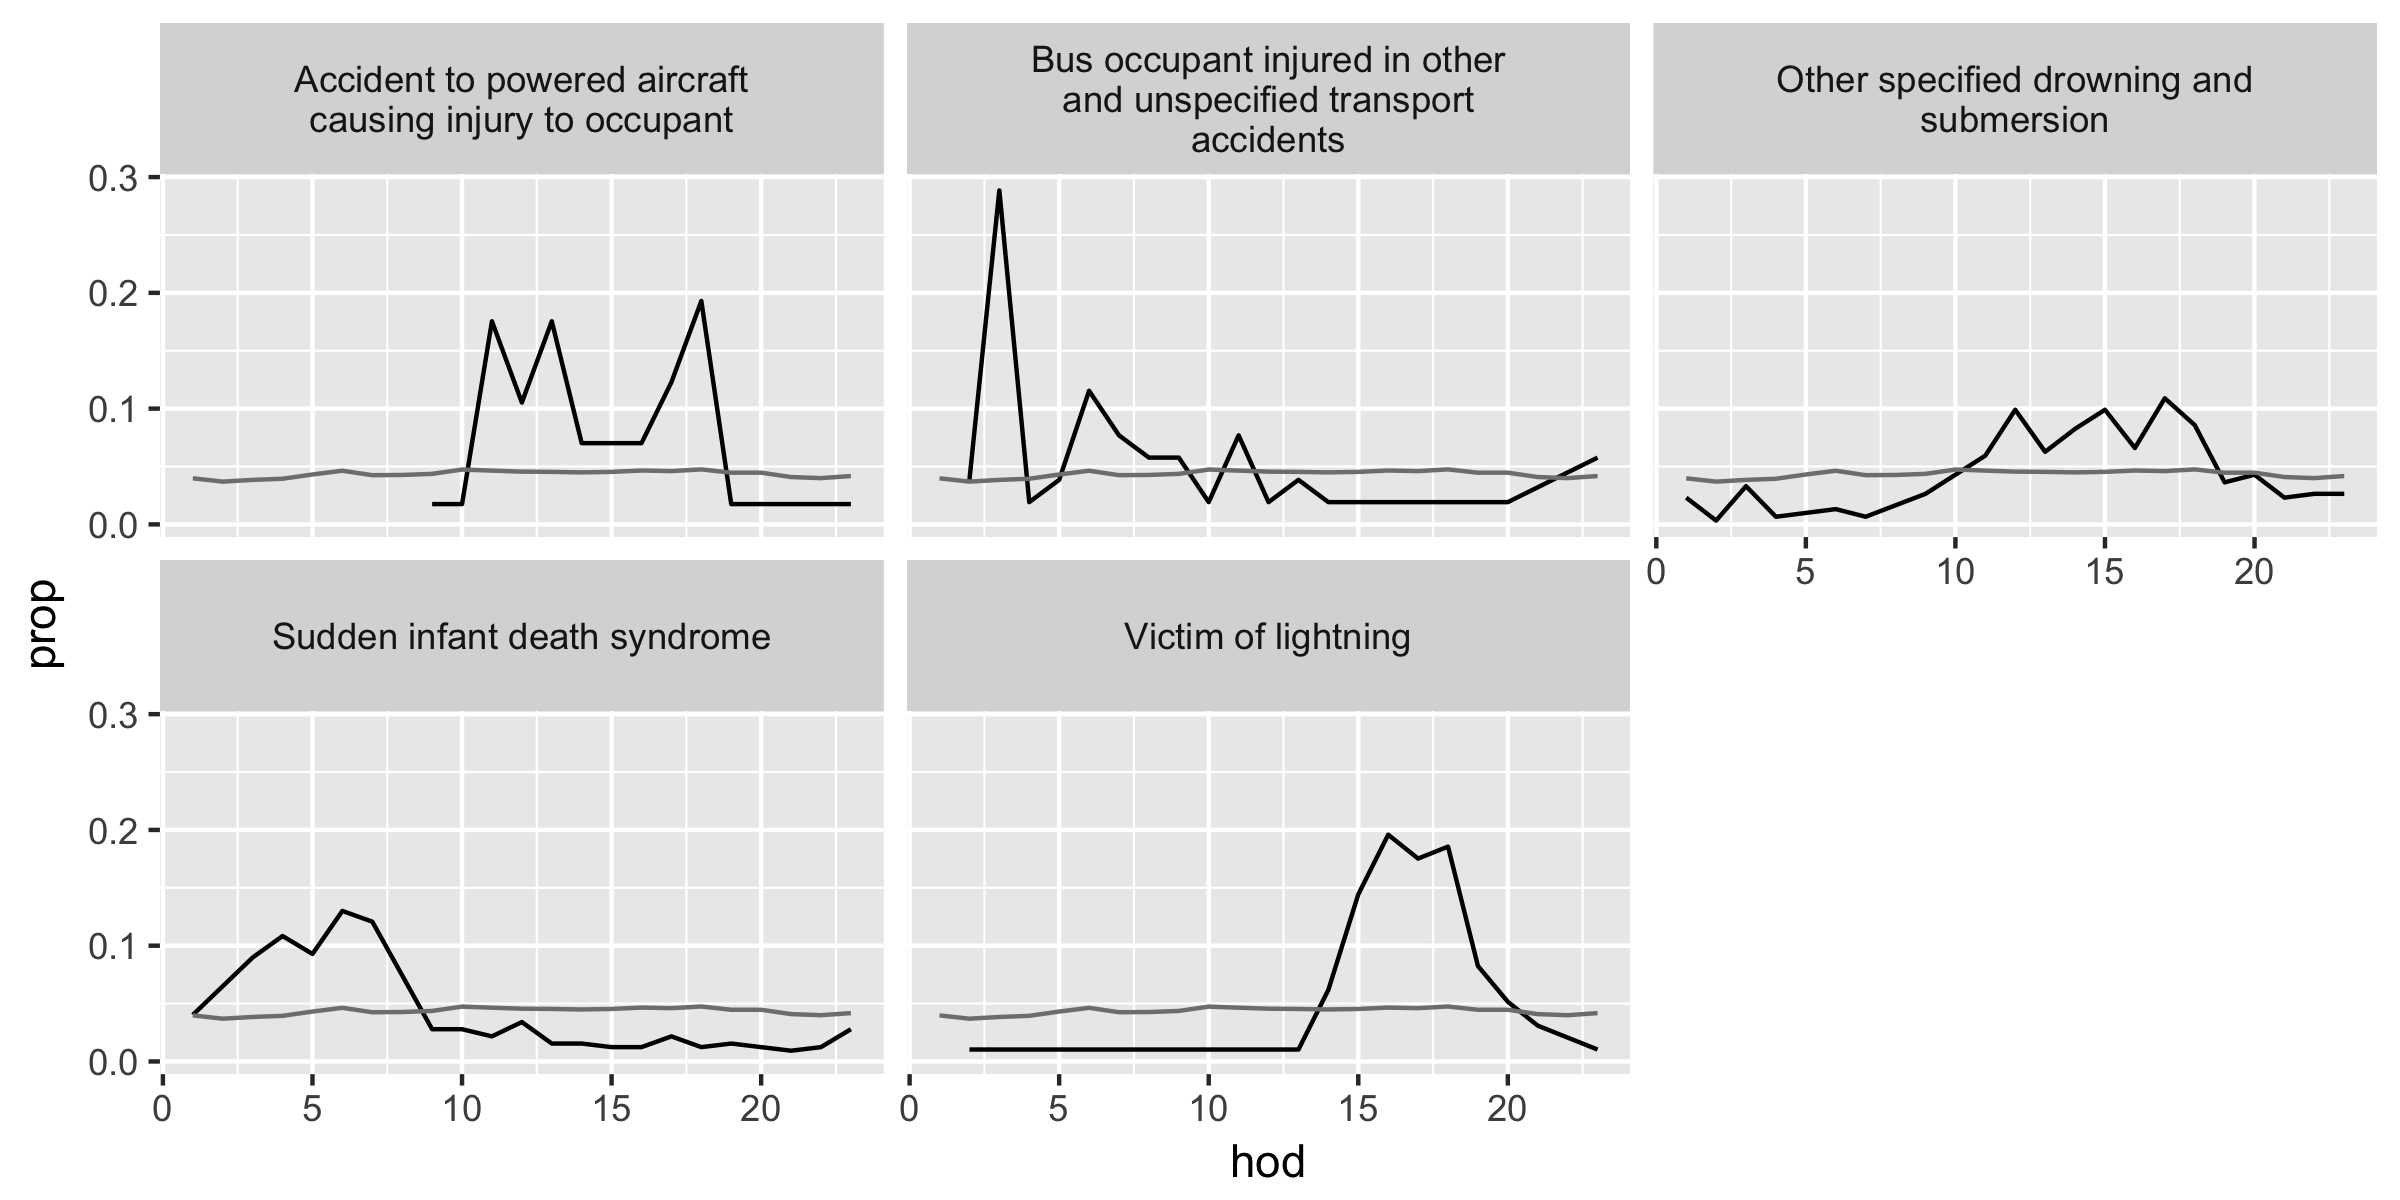
\includegraphics[width=1\linewidth]{tidy_case_study/unusual-sml} \end{center}

The first figure is the unusual causes of deaths in \texttt{devi\_cod}
with a relatively large number of deaths
(\texttt{n\ \textgreater{}\ 350}) and the second is that of a relatively
small number of deaths (\texttt{n\ \textless{}=\ 350}).

Hints

\begin{itemize}
\item
  Using the cuttoff value \texttt{resid\ \textgreater{}\ 1.5}, filter
  \texttt{devi\_cod} and call it \texttt{unusual} data frame. Join
  \texttt{master\_hod} and \texttt{unusual} data frames. Then create two
  subsets of data with conditions \texttt{n\ \textgreater{}\ 350} and
  \texttt{n\ \textless{}=\ 350}.
\item
  Use \texttt{ggplot()\ +\ geom\_line()} structure with
  \texttt{+\ facet\_warp(\textasciitilde{}\ disease,\ ncol\ =\ 3)}
\item
  To include the overall hourly proportions of deaths
  (\texttt{prop\_all}) representing the average of all causes of deaths
  in a given hour, add another layer by
  \texttt{geom\_line(aes(...),\ data\ =\ overall\_freq)} with a local
  \texttt{aes()} argument and a data argument. With the data argument,
  variables in another data frame can be combined (assuming the axes
  have the same measurements), and here we use the
  \texttt{overall\_freq} data frame from the panel (d) portion of Table
  16 above.
\item
  \texttt{last\_plot()\ \%+\%\ another\_data\_frame} reproduces a plot
  of the same structure with a different data frame
\end{itemize}

\subsection*{The Key}\label{the-key}
\addcontentsline{toc}{subsection}{The Key}

The solution will be presented at the workshop and later posted.

\section{Upcoming topics}\label{next}

\begin{itemize}
\item
  Statistical inferences with simulations
\item
  Linear regressions
\end{itemize}

\chapter{Resources}\label{resources}

Here are more resources for learning R.

\textbf{Free Books}

\begin{itemize}
\item
  \href{http://cran.r-project.org/doc/manuals/R-intro.pdf}{Official CRAN
  R Manual}
\item
  \href{http://www.statmethods.net/}{Quick R}
\item
  \href{http://heather.cs.ucdavis.edu/~matloff/132/NSPpart.pdf}{The Art
  of R Programming by Norman Matloff}
\item
  \href{https://ismayc.github.io/moderndiver-book/}{ModernDive}
\item
  \href{http://www.burns-stat.com/documents/tutorials/impatient-r/\#keyobjects}{Impatient
  R}
\item
  \href{http://cran.r-project.org/doc/contrib/Verzani-SimpleR.pdf}{Simple
  R by John Verzani}
\item
  \href{http://ipsur.org/install.html}{Introduction to Probability and
  Statistics Using R By Jay Kerns}
\item
  \href{https://en.wikibooks.org/wiki/R_Programming}{R Wikibook}
\item
  \href{http://www.cookbook-r.com/}{Cookbook for R by Winston Chang}
\item
  \href{https://togaware.com/onepager/}{OnePageR}
\item
  \href{http://www.burns-stat.com/documents/books/the-r-inferno/}{The R
  Inferno}
\end{itemize}

\textbf{Videos}

\begin{itemize}
\item
  \href{http://blog.revolutionanalytics.com/2012/12/coursera-videos.html}{Coursera's
  four week course videos}
\item
  \href{http://bitesizebio.com/webinar/20600/beginners-introduction-to-r-statistical-software/}{Workflow
  example video by Jermey Chacon}
\item
  \href{https://www.youtube.com/watch?v=cX532N_XLIs\&list=PLqzoL9-eJTNBDdKgJgJzaQcY6OXmsXAHU}{Video
  on Youtube}
\end{itemize}

\textbf{Tutorials}

\begin{itemize}
\item
  \href{https://www.tutorialspoint.com/r/index.htm}{R Tutorial}
\item
  \href{https://www.jaredknowles.com/r-bootcamp/}{R Bootcamp - Jared
  Knowles}
\item
  \href{http://tryr.codeschool.com/}{Step-by-step (sequential)
  interactive tutorial- Try R}
\item
  \href{http://swirlstats.com/students.html}{Another step-by-step
  interactive tutorial - swirl}
\end{itemize}

\textbf{With Small Fees: Tutorials from DataCamp}

\begin{itemize}
\item
  \href{https://www.datacamp.com/courses/cleaning-data-in-r}{Cleaning
  Data in R}
\item
  \href{https://www.datacamp.com/courses/dplyr-data-manipulation-r-tutorial}{Data
  Manipulation in R with dplyr}
\item
  \href{https://www.datacamp.com/courses/ggvis-data-visualization-r-tutorial}{Data
  Visualization in R with ggvis}
\item
  \href{https://www.datacamp.com/courses/data-visualization-with-ggplot2-1}{Data
  Visualization with ggplot2}
\end{itemize}

\textbf{Introduction to Coding}

\begin{itemize}
\tightlist
\item
  \href{http://toridykes.com/blog/2015/10/25/coding-resources-for-beginners\#.WMf84xCNooE}{Coding
  Resources for Beginners by Tori Dykes}
\end{itemize}

\bibliography{book.bib,articles.bib,packages.bib}


\end{document}
